\documentclass[../Main.tex]{subfiles}
\usepackage{multicol}

\begin{document}
\chapter{Application Architecture}

\intro{

}

\defn{Software Architecture}{
    The fundamental organization of a system is embodied in its components, their relationships to each other, and to the environment, and the principles guiding its design and evolution.  (ISO/IEC/IEEE 42010, November 2011 )
    There exist three definitions:
    \begin{itemize}
        \item Structure (elements, properties, relationships)
        \item decision rationale
        \item both
    \end{itemize}
}

\begin{enumerate}
    \item Bass, Clements and Kazman focuses on \textbf{structure}
    for example with architecture elements with their properties
    and relationships
    \item Jansen and Bosch empasizes design rational specifically
    \textbf{desicion outcome} and their justifications
    \item ISO/IEC/IEEE is a \textbf{hybrid definition} that combines elements from the other two
\end{enumerate}

Also Application Architecture as a sub-disiple of Software Architecture
that takes a logical viewpoint on end user apps and their architectures.
IT Architecture covers hardware and software and therefore is a superset.
(\href{https://arc42.org/overview}{ARC42 Software Architecture Templates}),
(\href{https://martinfowler.com/eaaCatalog/index.html}{Fowler's Enterprise Architecture}),
(\href{https://martinfowler.com/eaaDev/uiArchs.html}{Fowler's GUI Architectures})

Design challenges for the architecture of large and complex projects are divers and could contain:
\begin{itemize}
    \item User and channel diversity
    \item Process and resource integrity
    \item Integration need due to heterogeneity
    \item Complex data/domain models and processing rules
\end{itemize}

\section{Requirement Engineering}
\subsection{Architecural Significant Requirements}
All architecture is design, but not all design is architecture according to Grady Booch;
hence, it has to be decided what is in and out of scope of any architectural activity.
The notion of architectural significance has this purpose; it is a property of the requirements
that are elicited/stated for a particular system and/or project, as well as design elements
and decisions considered along the way. First and foremost, these requirements are non-functional
ones (also known as quality attributes); however, limiting architectural significance to these quality
attributes is an oversimplification. Functional requirements can be architecturally significant as
well, for instance if a feature request leads to the need for an additional external data provider
that has to be inte grated via an Application Programming Interface (API).
\defn{ASR Test}{
    \begin{enumerate}
        \item The requirement is directly associated with high business value or business risk
        \item The requirement is a concern of a particularly important stakeholder (for instance, the project sponsor or an external compliance auditor). 
        \item The requirement has runtime Quality-of-Service (QoS) characteristics (e.g., performance needs) that deviate from those already satisfied by the evolving architecture substantially.
        \item The requirement causes new or deals with one or more existing external dependencies that have unpredictable, unreliable and/or uncontrollable behavior. 
        \item The requirement has a cross-cutting nature and therefore affects multiple parts of the system and their interactions; it may even have system-wide impact. 
        \item The requirement has a first-of-a-kind character: e.g., the team has never built a component before that satisfies this particular requirement. 
        \item The requirement has been troublesome and caused critical situations, budget overruns or client dissatisfaction in a previous project in a similar context. 
    \end{enumerate}
    Point \textbf{1 to 2} handles \textbf{business value risks} and \textbf{3 to 7} focuses mainly on \textbf{technical risks}.
    \href{https://medium.com/olzzio/architectural-significance-test-9ff17a9b4490}{ZIO}
}
S. Toth asks the following five questions to classify the architectural significance of decisions that justify if and
how a requirement is met.
\textbf{Just Enough Software Architecture}:
\begin{enumerate}
    \item Is the decision hard to change later?
    \item Is the decision expensive to implement or execute?
    \item Are demanding, qualitative requirements stated?
    \item Are requirements difficult to map to existring solutions or experiences?
    \item Is the experience in the solution space weak?
\end{enumerate}

Assessment of architectural significance scopes and prioritizes architecture analysis, 
synthesis/design, and evaluation/review. NFRs should be specified in a SMART way.


\begin{table}[h]
    \centering
    \begin{tabular}{|c|c|c|c|}
    \hline
    Requirement & Score & Mapping & Explanation \\
    \hline
    Autoscaling & H & RC-2 & Justification \\
    \hline
    \end{tabular}
    \caption{Example ASR Test}
\end{table}


\subsection{NFR Catalogs and Taxonomies}
The SMART criteria are frequently used in project and people management, but they can also be applied to Non
Functional Requirement (NFR) engineering. Most of the time only S and M are used in NFR engineering.

\defn{SMART}{
\begin{description}
    \item[Specific]  Targeting a particular area for improvement. Which feature or part of the system should satisfy the requirement?
    \item[Measurable] Quantifying, or at least suggesting, an indicator of progress. How can testers and other stakeholders find out whether the requirement is met (or not)? Is the 
    requirement quantified?
    \item[Agreed Upon] The goal must be realistic and achievable and have a consent in the team (everyone should know
    what we are talking about).
    \item[Realistic] Outlining attainable results with available resources. Time-related: Including a timeline for expected results
    \item[Time-Bound] There should be a clearly defined timeline, including a starting date and a target date.
\end{description}
The specific definitions of the words are not fixed.
A, R, T are requirements engineering and project management concerns.
}

The FURPS+ acronym, devised by Robert Grady of HP, provides a way to define requirements by non-functional
stories, and also provides a good way to categorize such needs. The breakdown here suggests some representative
questions around potential needs.
\defn{FURPS+}{
    Furps+:
    \begin{itemize}
        \item Functionality
        \item Usability
        \item Reliability
        \item Performance
        \item Supportability
        \item Design constraints
        \item Implementation constraints
        \item Physical constrains
        \item Interface contraints
    \end{itemize}
    \href{https://ieeexplore.ieee.org/document/4384163}{Martin Glinz}
}

\begin{figure}[H] 
    \centering
    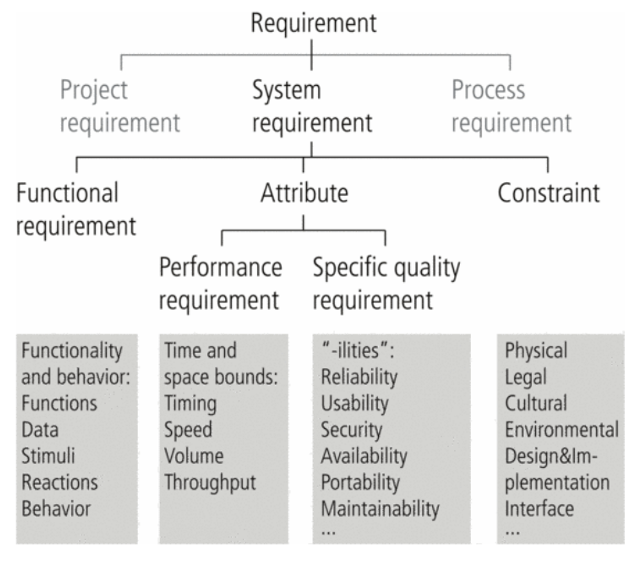
\includegraphics[width=0.5\linewidth]{Images/req-categorization.png}
    \caption{Requirement Categorization}
\end{figure}

\newpage
\subsection{Quality Attribute Scenario (QAS)}
There are a variety of published taxonomies and definitions and 
architectural there are three problems with system quality attributes:
\begin{enumerate}
    \item The definitions provided for an attribute are not operational.
    \item To which quality does a particular aspect belong. Is a system failure an aspect
    of availability, an aspect of security, or an aspect of usability?
    \item Each attribute community has developed its own vocabulary.
\end{enumerate}

We use two general solution for these problems:
\begin{description}
    \item[First two problems:] (nonoperational definitions and overlapping attribute concerns) Use
    Quality Attribute Scenarios as a means of characterizing quality attributes.
    \item[Third problem:] Provide a brief discussion of each attribute — concentrating on its underlying
    concerns — to illustrate the concepts that are fundamental to that attribute community.
\end{description}

Quality attributes describe how a system provides its functionality, not how.
It can be used to achieve S and M n SMART.
Measurability is enabled by the "Response Measure field" specificity by the other fields.

\begin{figure}[H] 
    \centering
    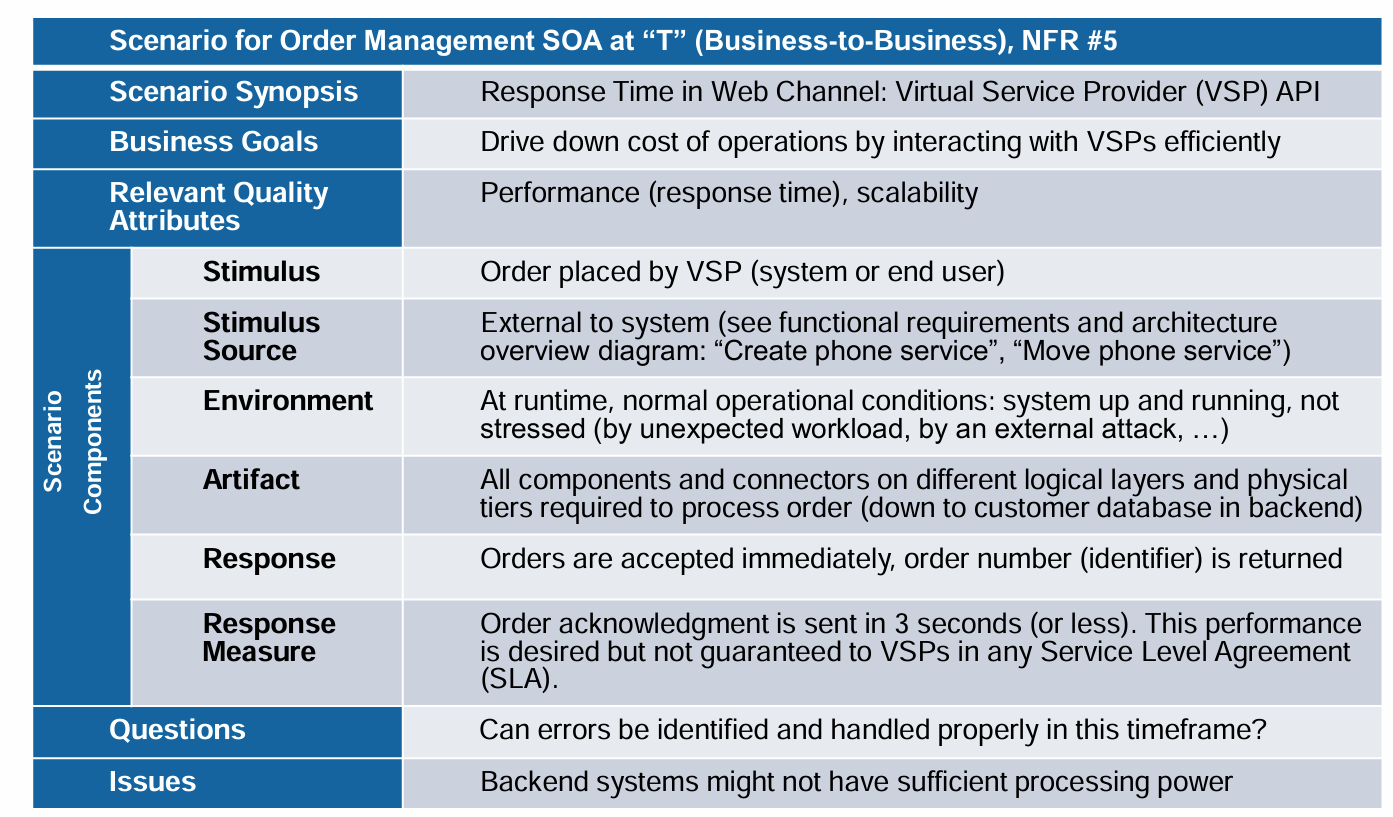
\includegraphics[width=1\linewidth]{Images/qas.png}
    \caption{QAS Example}
\end{figure}
\newpage
\begin{figure}[H] 
    \centering
    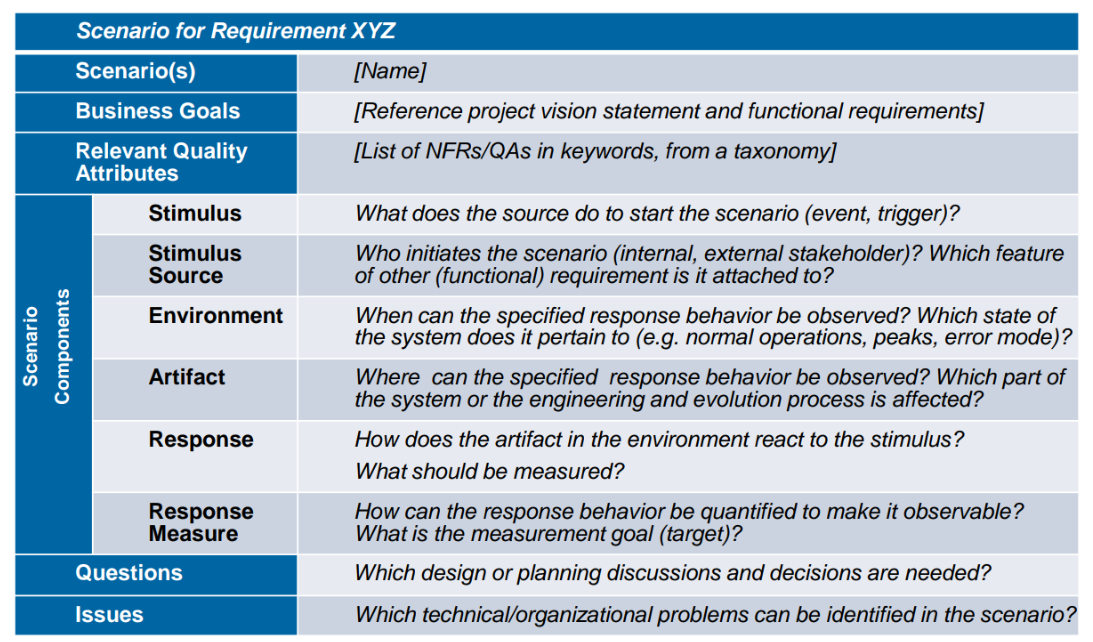
\includegraphics[width=1\linewidth]{Images/qas-template.png}
    \caption{QAS Empty Template}
\end{figure}
\begin{figure}[H] 
    \centering
    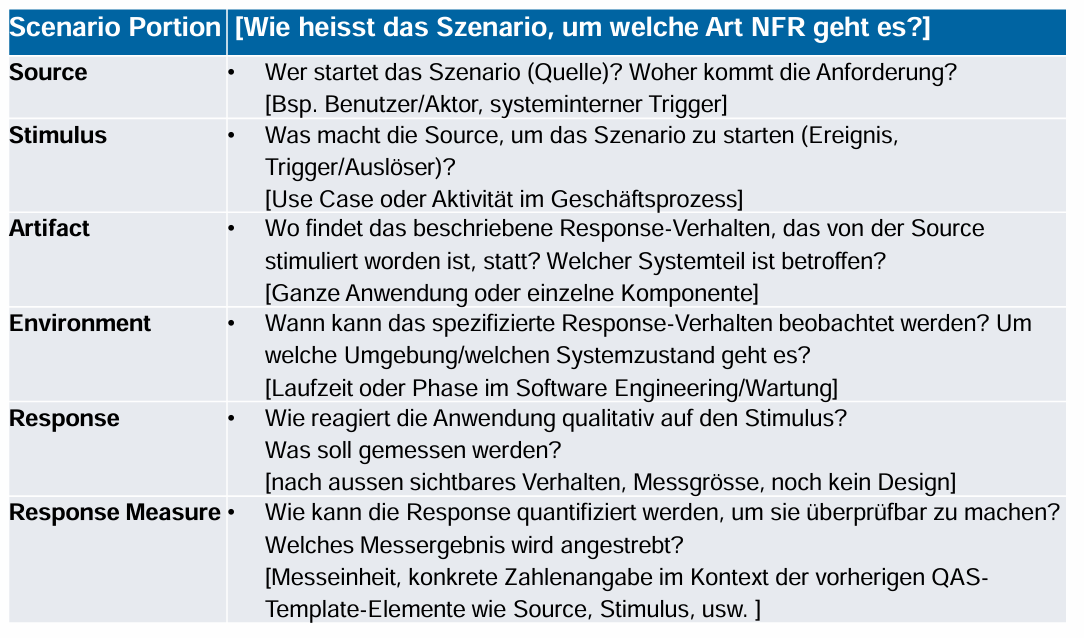
\includegraphics[width=1\linewidth]{Images/qas-template-2.png}
    \caption{QAS Template Description}
\end{figure}
\newpage
\subsection{Landing Zones}
Rather than establishing one measurable target, define three.
This helps agree upon a range rather than one single value.
This is similar to release criteria but allows for tolerances
in acceptable values. Moreover it allows for some flexibility
in meeting goals. This can be used without QAS.
\\\\
Goal:  Establish three measurable \textbf{(M)} values rather than a single measure that might not be realistic \textbf{(R)} and
impossible to agree upon \textbf{(A)}.

\begin{figure}[H]
    \centering
    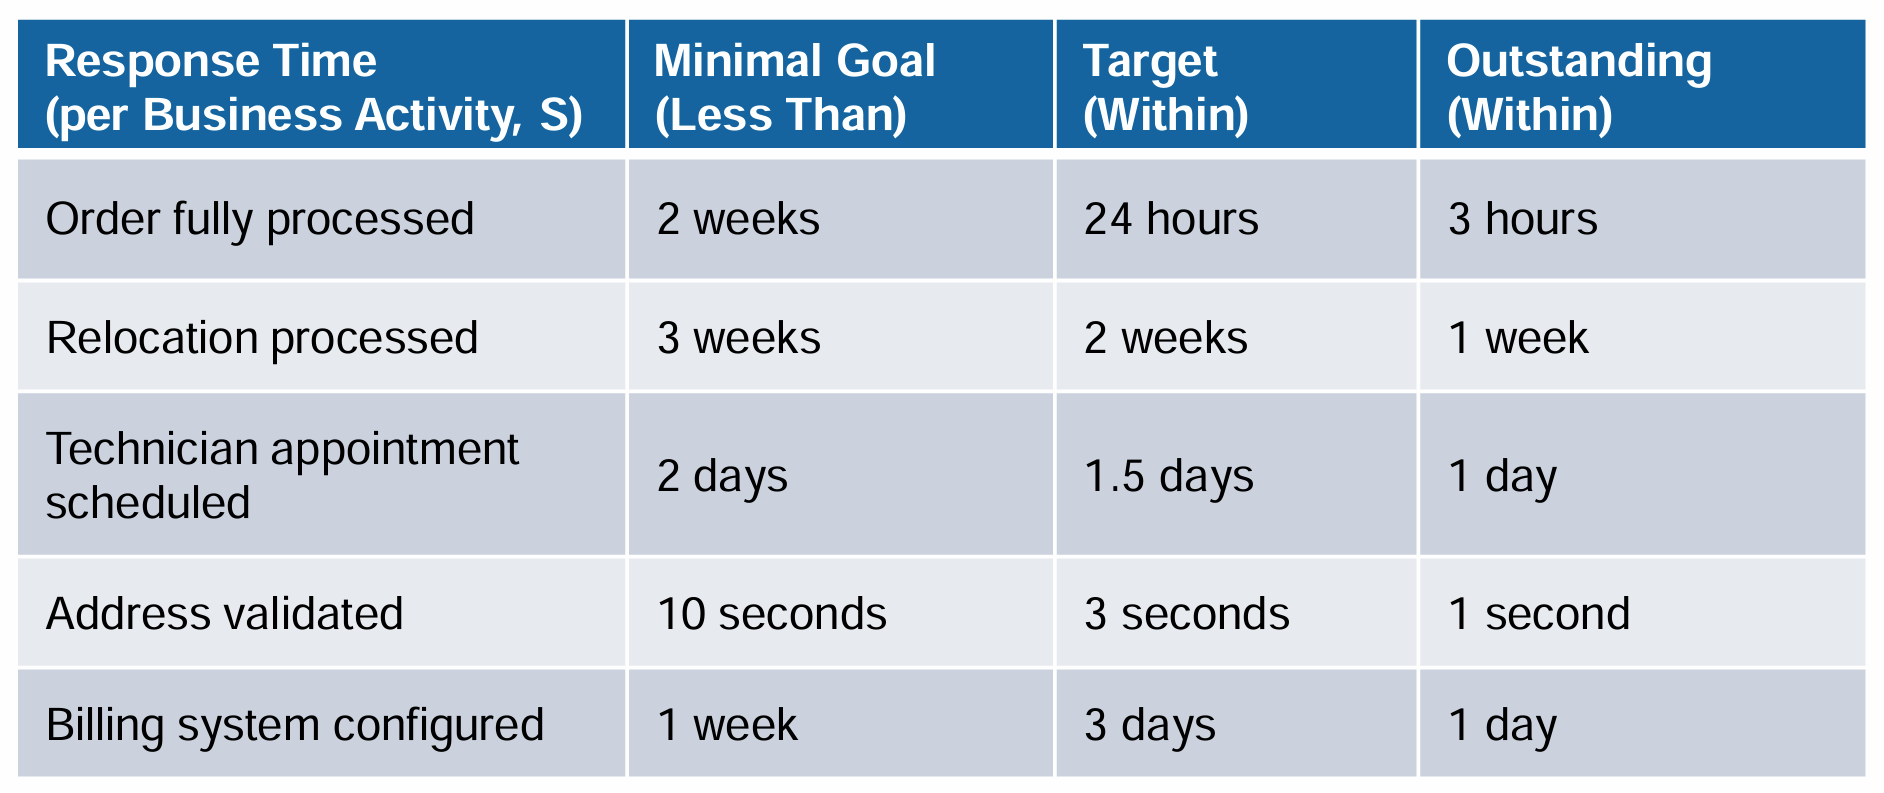
\includegraphics[width=1\linewidth]{Images/landingzone.png}
    \caption{Landing Zones}
\end{figure}

\subsection{System Context Diagrams}
SCD should be use to identify external dependencies.
In this method we represent systems as black boxes and
depict interactions with external entities.
It can identity the information and control flow.

\begin{figure}[H]
    \centering
    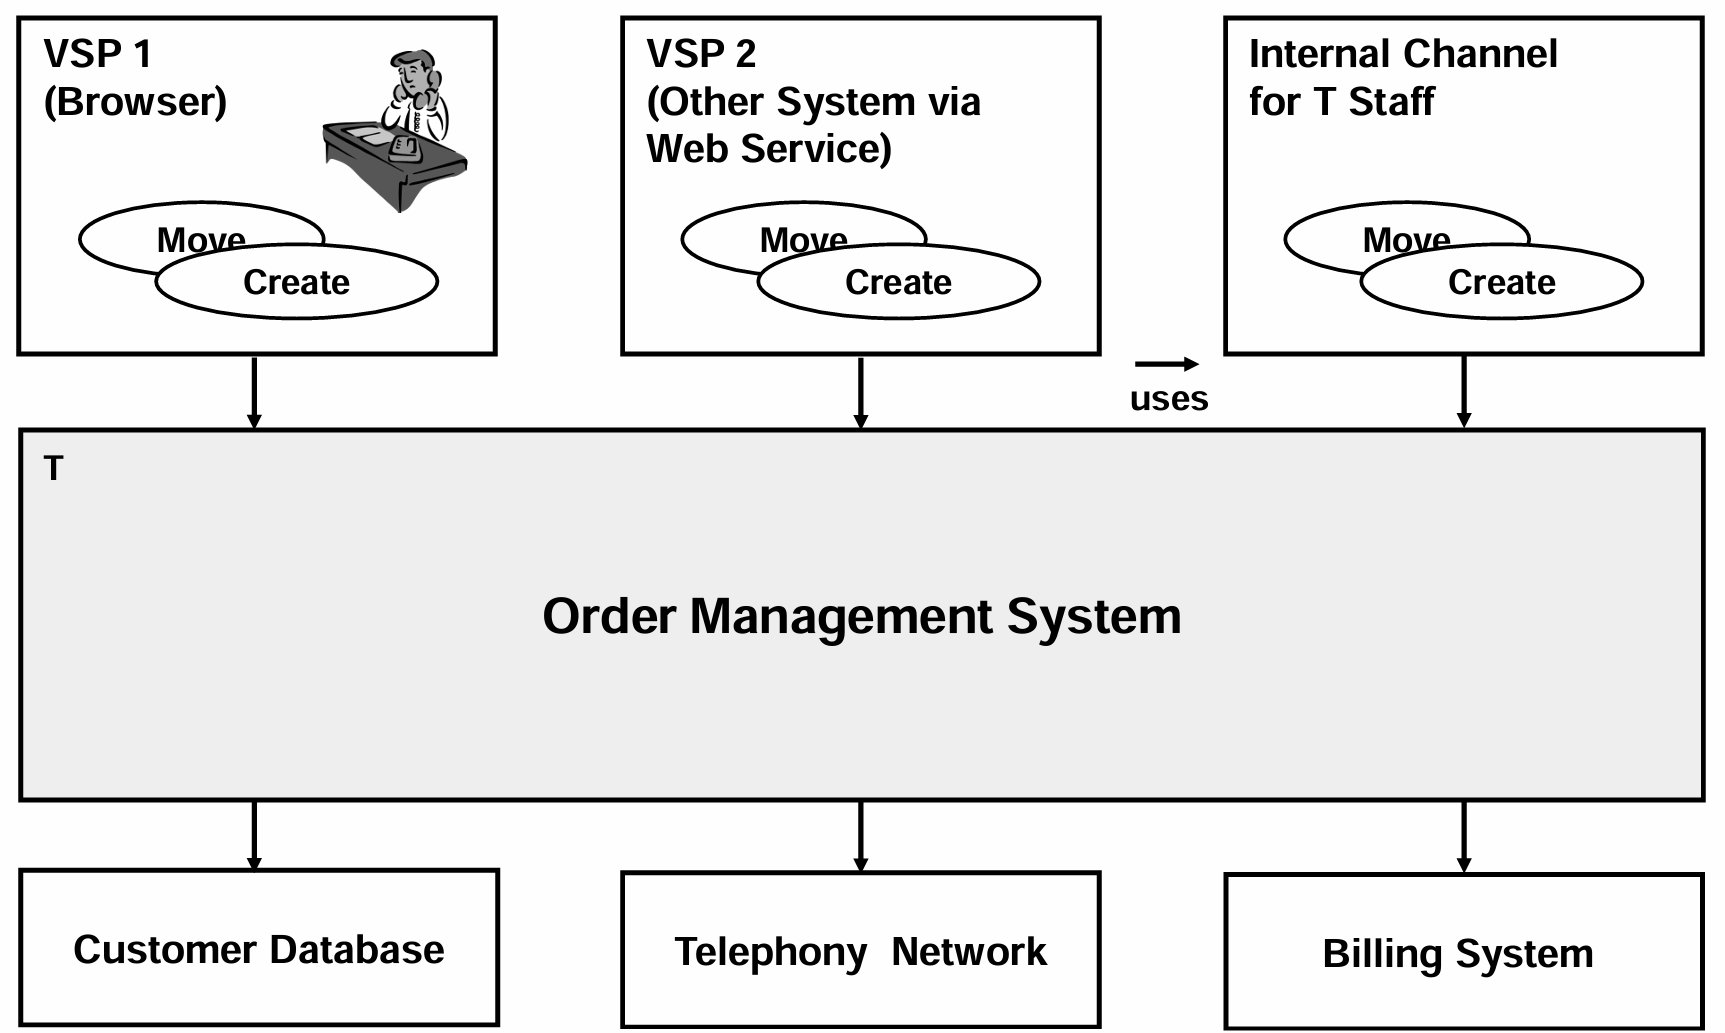
\includegraphics[width=0.65\linewidth]{system-context-example.png}
    \caption{System Context Diagram Example}
\end{figure}

%\subsection{Twin Peaks}
% Analysis and synthesis do not follow each other in a waterfall
% Cross fertilization, you learn as you go: “Twin Peaks” Model
%\begin{figure}[H]
%    \centering
%    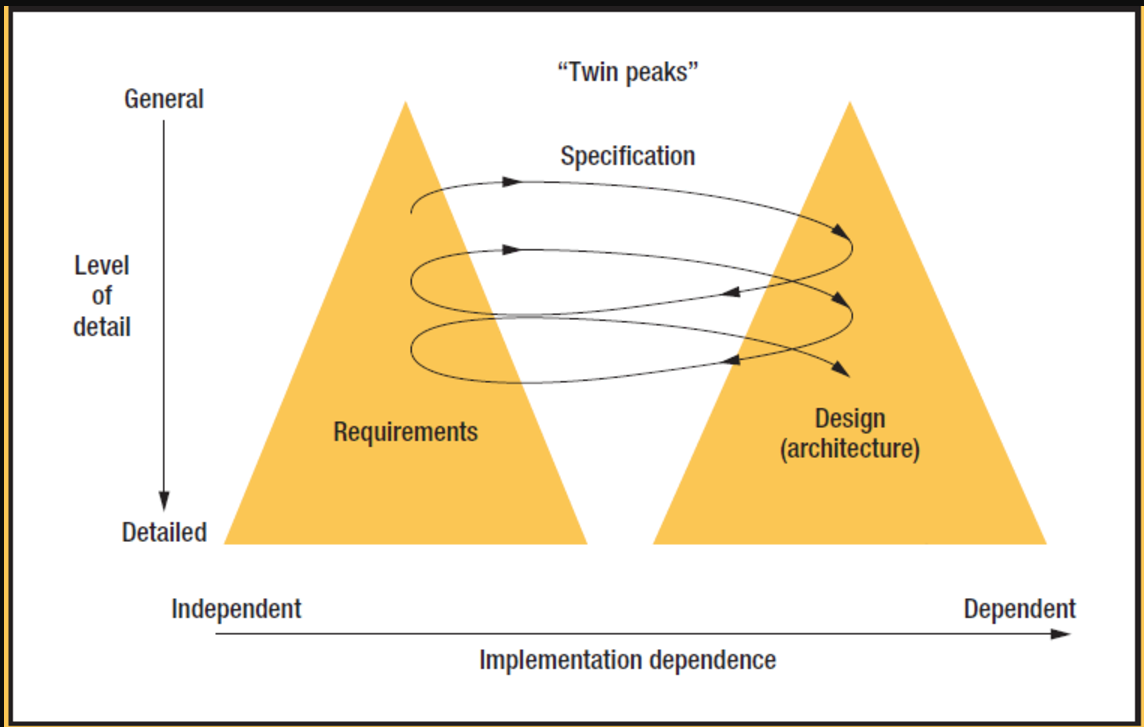
\includegraphics{Images/twinpeak.png}
%    \caption{Twin Peak Design}
%    \label{fig:twinpeakdesign}
%\end{figure}
%\newpage

\newpage

\subsection{Quality Utility Trees}
Quality Utility Trees (QUT) can be used to refine
each toplevel taxonomy topic. In the trees the leaves
represent QAS prioritized by \textbf{value and risk} with classes low, medium and high (l,m,h).

\begin{figure}[H]
    \centering
    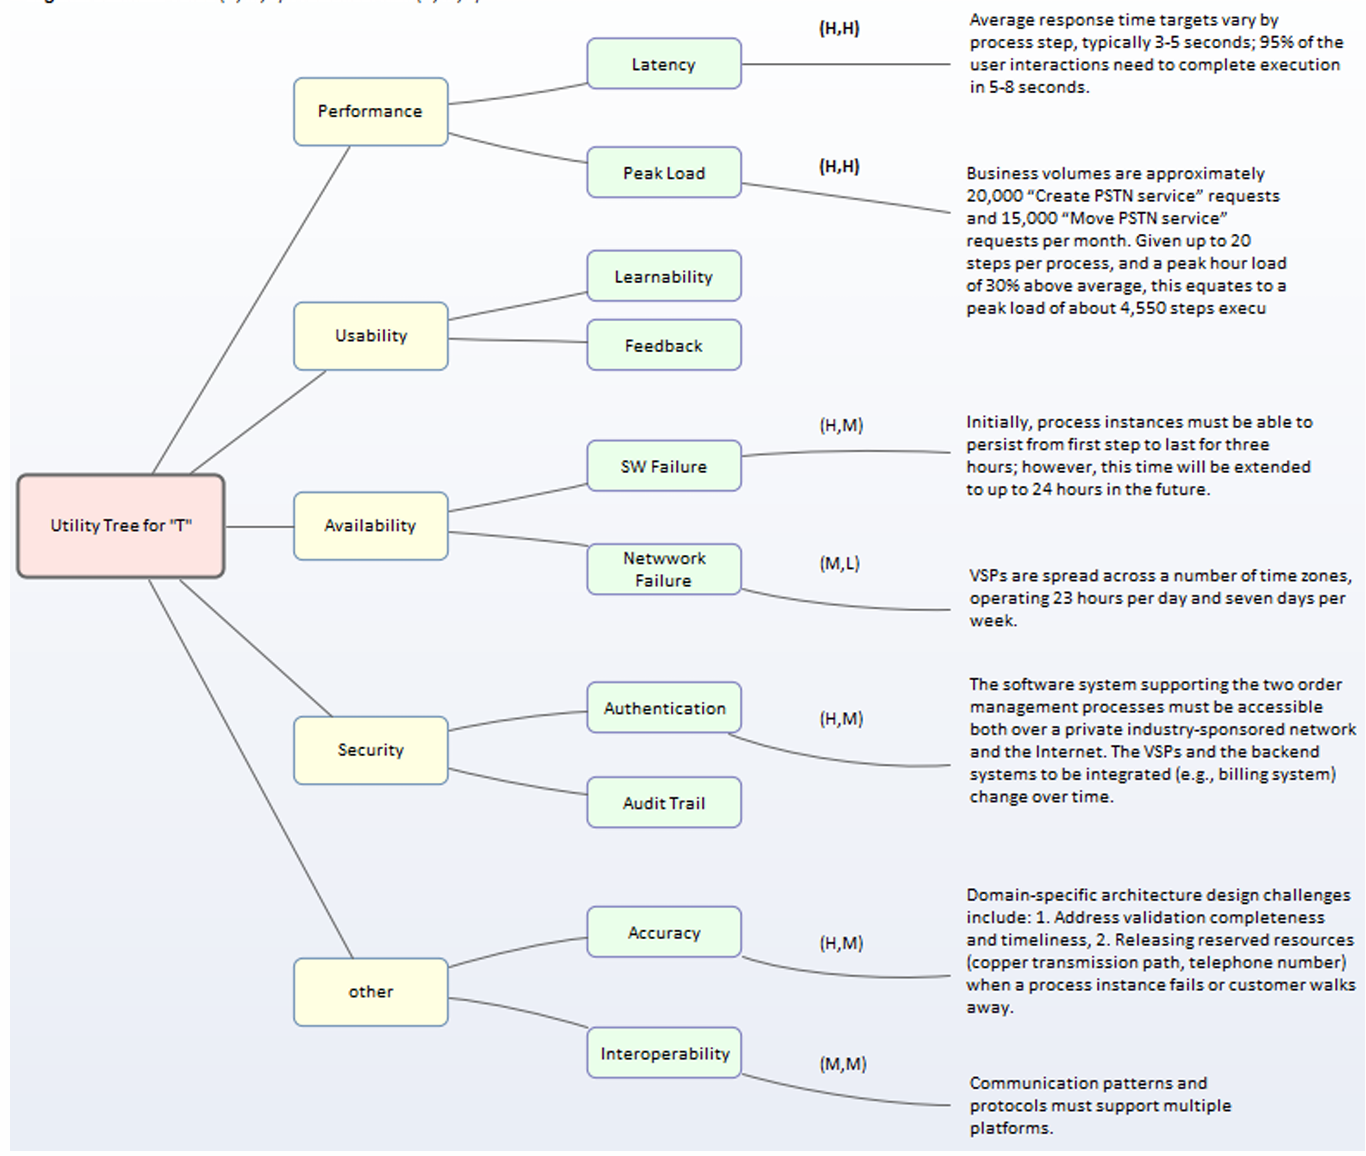
\includegraphics[width=1\linewidth]{quality-utility-trees.png}
    \caption{Quality Utility Trees}
\end{figure}
\newpage

\section{Solution Strategy}
The term Solution Strategy is from Gernat Starke (arc42).
It corresponds to the Inception and Elaboration phases in
RUP. It includes the \textbf{big decisions}
one should make to which would later be costly to change (Grady Booch).
IBM defines some reference goals for the solution stategy:
\begin{itemize}
    \item Provide a single place to find important decisions
    \item Make explicit the rationale and justification
    \item Preserve design integrity
    \item Ensure that architecture is extensible and evolving
    \item Provide a reference of documented decisions
    \item Aboid unnecessary reconsideration of the same issues
\end{itemize}

Creation of a Solution Strategy is the first step in architecture design.
It is ASR-driven (incl. NFRs) and can be refined and adapted throughout project.
Further help can be found in Step/section 4 in arc42 template for architecture descriptions.

Decisions Made in Solution Strategy:
\begin{itemize}
    \item Logical layers bring flexibility and support division of labor
    \item Client/Server Cuts (CSCs) with five options to place logical layers on tiers;  CSCs can be combined for 
    performance, reliability, scalability 
    \item Many other patterns also eligible as conceptual solution options
    \item We use container diagrams, the second C in C4, for high-level, white box view.
    There layers and tiers as well as key technologies can be mentioned/outlined
\end{itemize}

\defn{Solution Strategy (arc42)}{
Are fundamental decisions and solution strategies,
that shape the system's architecture. These include:
\begin{itemize}
    \item Technology decisions
    \item Decisions about the top-level decomposition of the system, e.g. usage of an architectural pattern or design pattern
    \item Decisions on how to achieve key quality goals
    \item Relevant organizational decisions, e.g. selecting a development process or delegating certain tasks to third parties.
\end{itemize}
 \href{https://docs.arc42.org/section-4/}{ARC42 SS Template}
}

\defn{Big Architectural Decisions}{
    \begin{enumerate}
        \item Those with high arch. significance score
        \item Those requiring financial investment; those with tough consequences
        \item Those that take a long time to execute upon
        \item Those with many or still unclear outgoing dependencies
        \item Those that take a long time to make according to DoD (ecADR)
        \item Those with a high level of abstraction 
        \item Those with problem/solution space outside of team's comfort zone 
    \end{enumerate}
}
For reference documentation use the template \href{https://github.com/adr/madr}{MADR Templates}.

\subsection{Y-Template (Stating Decisions)}
The Y-Template can be used to make decisions more
descriptive. It links AD to design context and NFRs
and shows tradeoffs between qualities.

\begin{figure}[H]
    \centering
    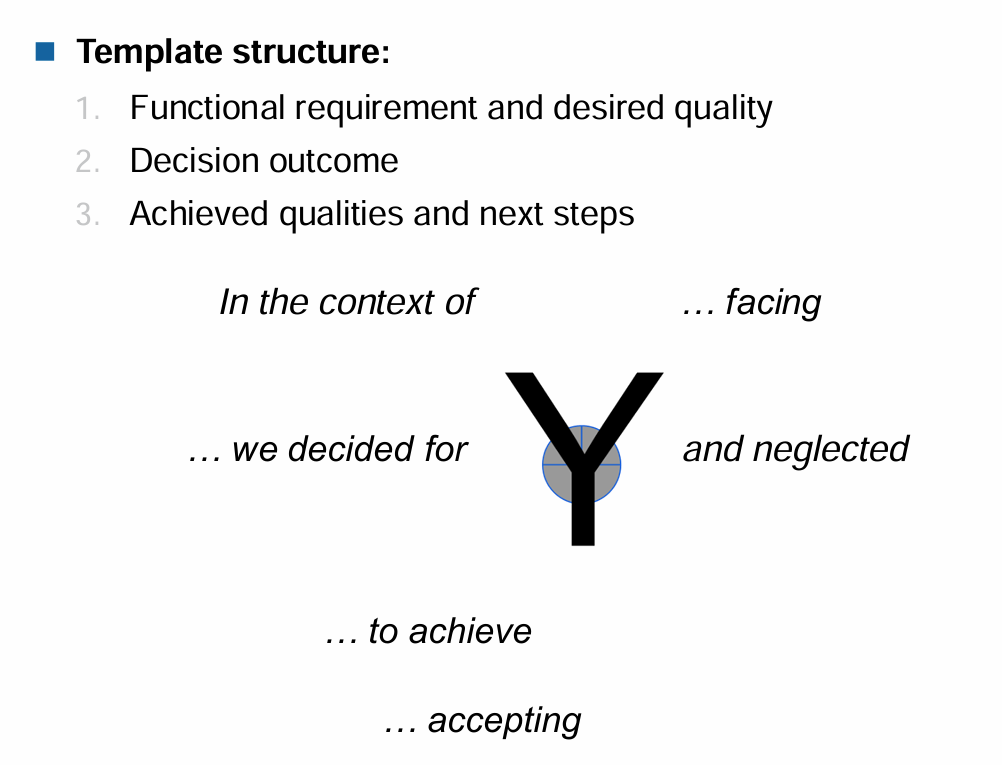
\includegraphics[width=0.75\linewidth]{Images/yarchitecturedesign.png}
    \caption{Y-Template for Architecture Design Decision}
\end{figure}

%\subsection{Architectural Decision Records}
%\href{https://adr.github.io/}{ADR Templates}

\subsection{Logical Layering and Tiers}

\begin{figure}[H]
    \centering
    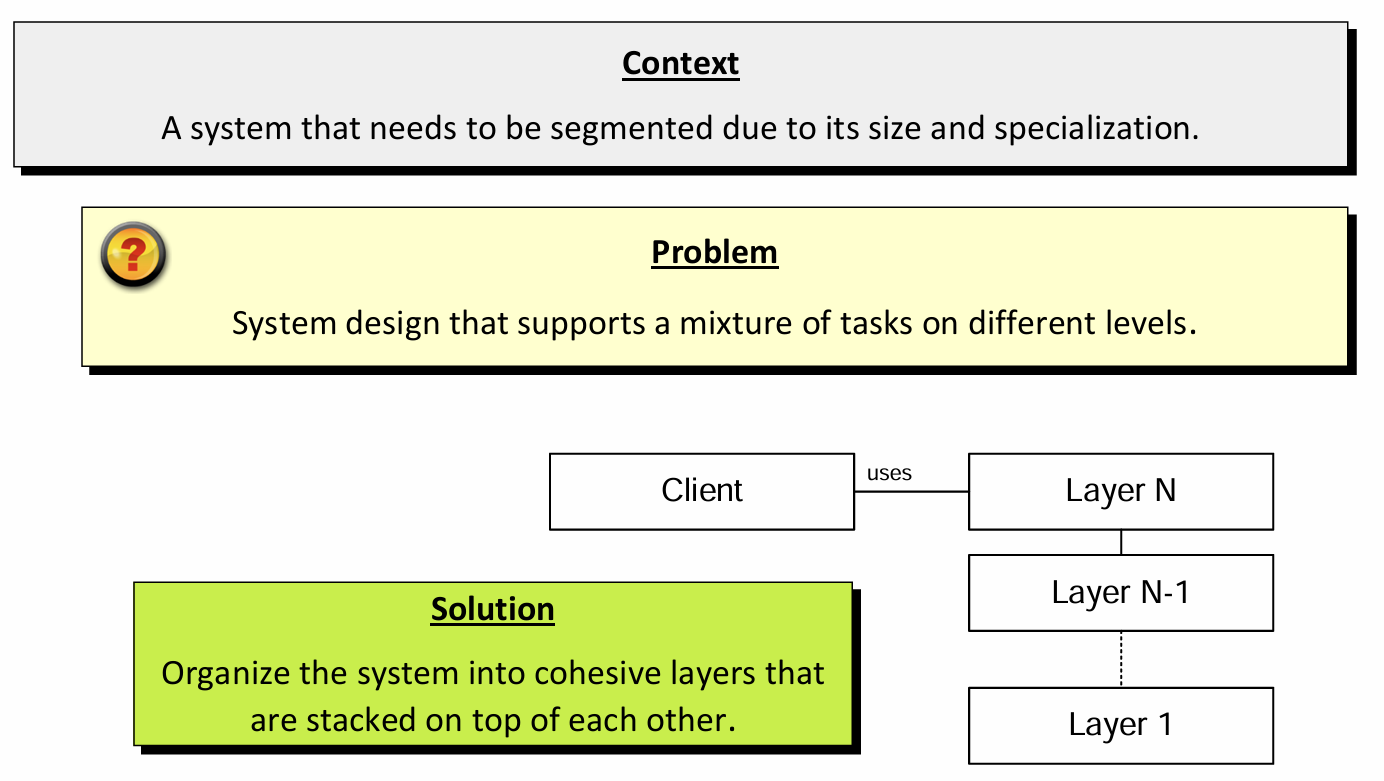
\includegraphics[width=0.75\linewidth]{Images/logicallayering.png}
    \caption{Logical Layering}
\end{figure}

The definition of layers and tiers is a typical
big decision in solution strategy:
\defn{Layers and Tiers}{
    \begin{description}
        \item[Layers]  describe the logical groupings 
        of the functionality and components in an application.
        In the logical and implementation view, \textbf{they separate concerns}.
        \item[Tiers] describe the physical distribution of the 
        functionality and components on separate servers, 
        computers, networks, or remote locations.
        In the process and physical view, they \textbf{distribute the workload}.
    \end{description}
}

Although both layers and tiers use the same set of names 
(presentation, business, services, and data), 
remember that only tiers imply a physical separation.
It is quite common to locate more than one layer on the
same physical machine (the same tier). You can think of
the term tier as referring to physical distribution
patterns such as two-tier, three-tier, and n-tier.
The following architectural drivers and decision making criteria (or forces in pattern terminology) apply:
\begin{itemize}
    \item Business needs vs.construction complexity
    \item Processing style: online (transactional) vs. offline (batch processing)
    \item Distribution vs. performance, security, consistency
    \item Software distribution cost
    \item Reusability vs. performance vs. complexity
    \item Supportability
\end{itemize}

\defn{Typical Layering}{
    An often used logical layering scheme is:
    \begin{itemize}
        \item Presentation Layer
        \item Business Logic Layer
        \item Data Access Layer
    \end{itemize}
}
Its most popular in enterprise application development but also applicable in other genres.
The layer pattern itself does not imply process/server boundary and any use of remoting is optional.

%\begin{description}
%\item[Presentation Layer:] End users and external systems only talk to presentation layer. Rationale: isolation from backend. Presentation layer talks to business logic. Rationale: support multiple presentations of same logic
%\item[Business Logic:] Business logic uses data access layer to communicate with database and backend systems. Which can be swapped in and out
%\end{description}

\begin{figure}[H]
    \centering
    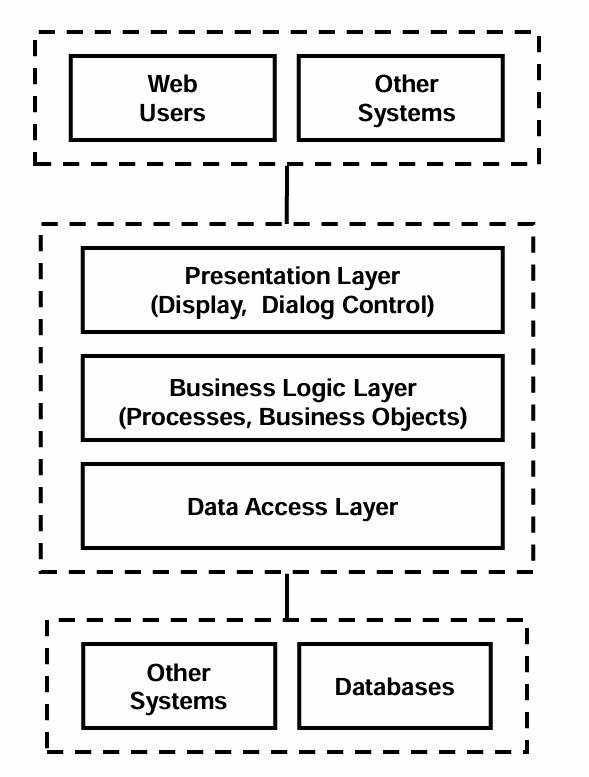
\includegraphics[width=0.4\linewidth]{Images/logicallayer.png}
    \caption{Logical Layers}
\end{figure}

This figure follows Fowlers approach to layers.
There are many options how to assign layers to tiers: Layer boundary or
within layer,  Single or multiple assignments.

\newpage
\subsection{Client Server Cuts (CSC)}
The five CSCs have been captured as distribution patterns 
rather early in the evolution of object-oriented pro gramming
and integrated business information systems (Renzel and Keller (1997)).
\begin{figure}[H]
    \centering
    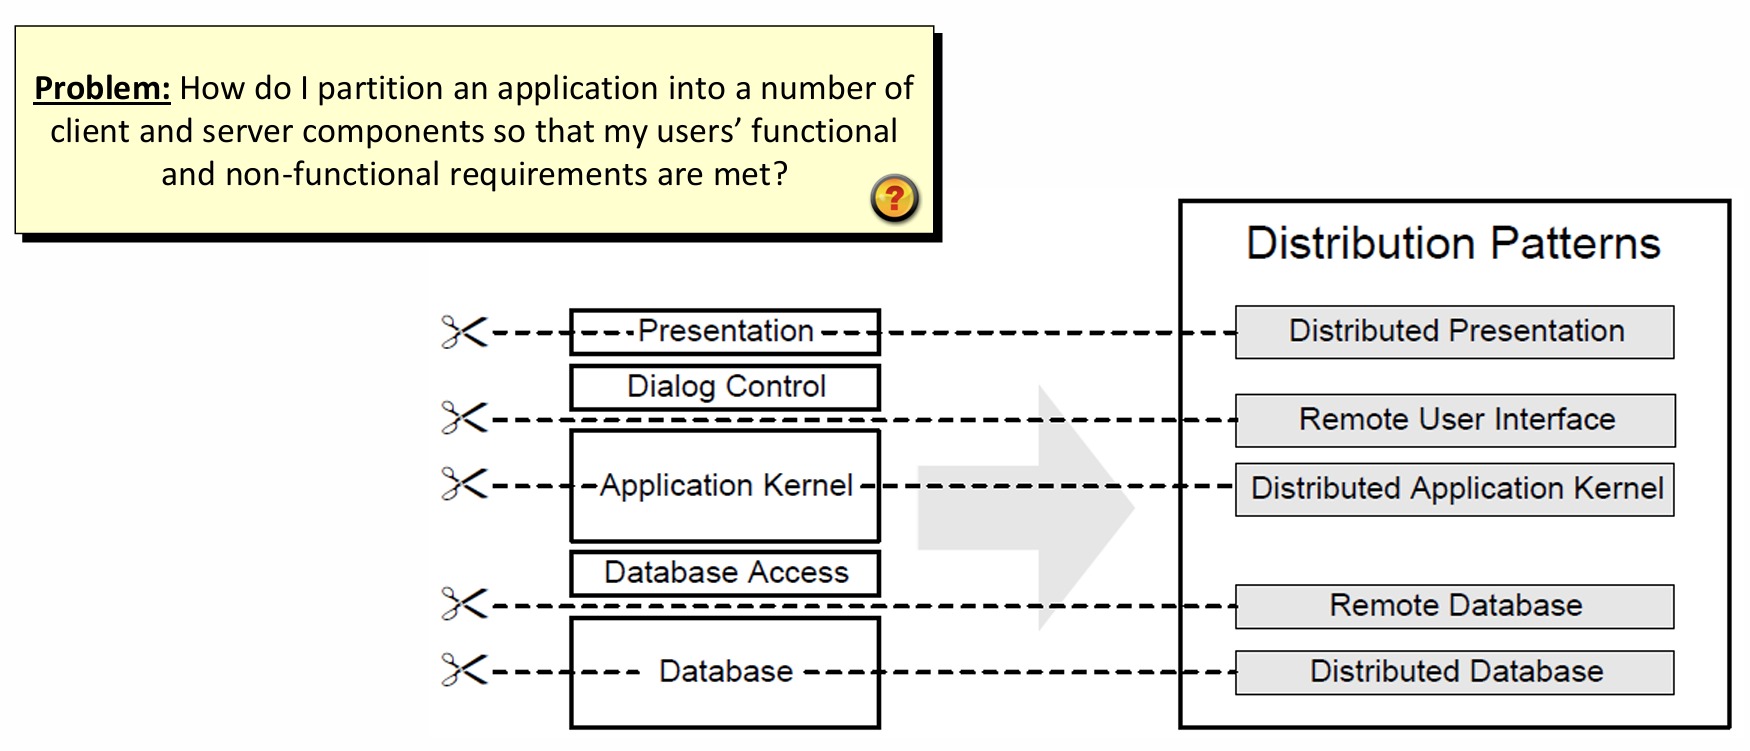
\includegraphics[width=1\linewidth]{Images/csc.png}
    \caption{CSC}
\end{figure}

\begin{figure}[H]
    \centering
    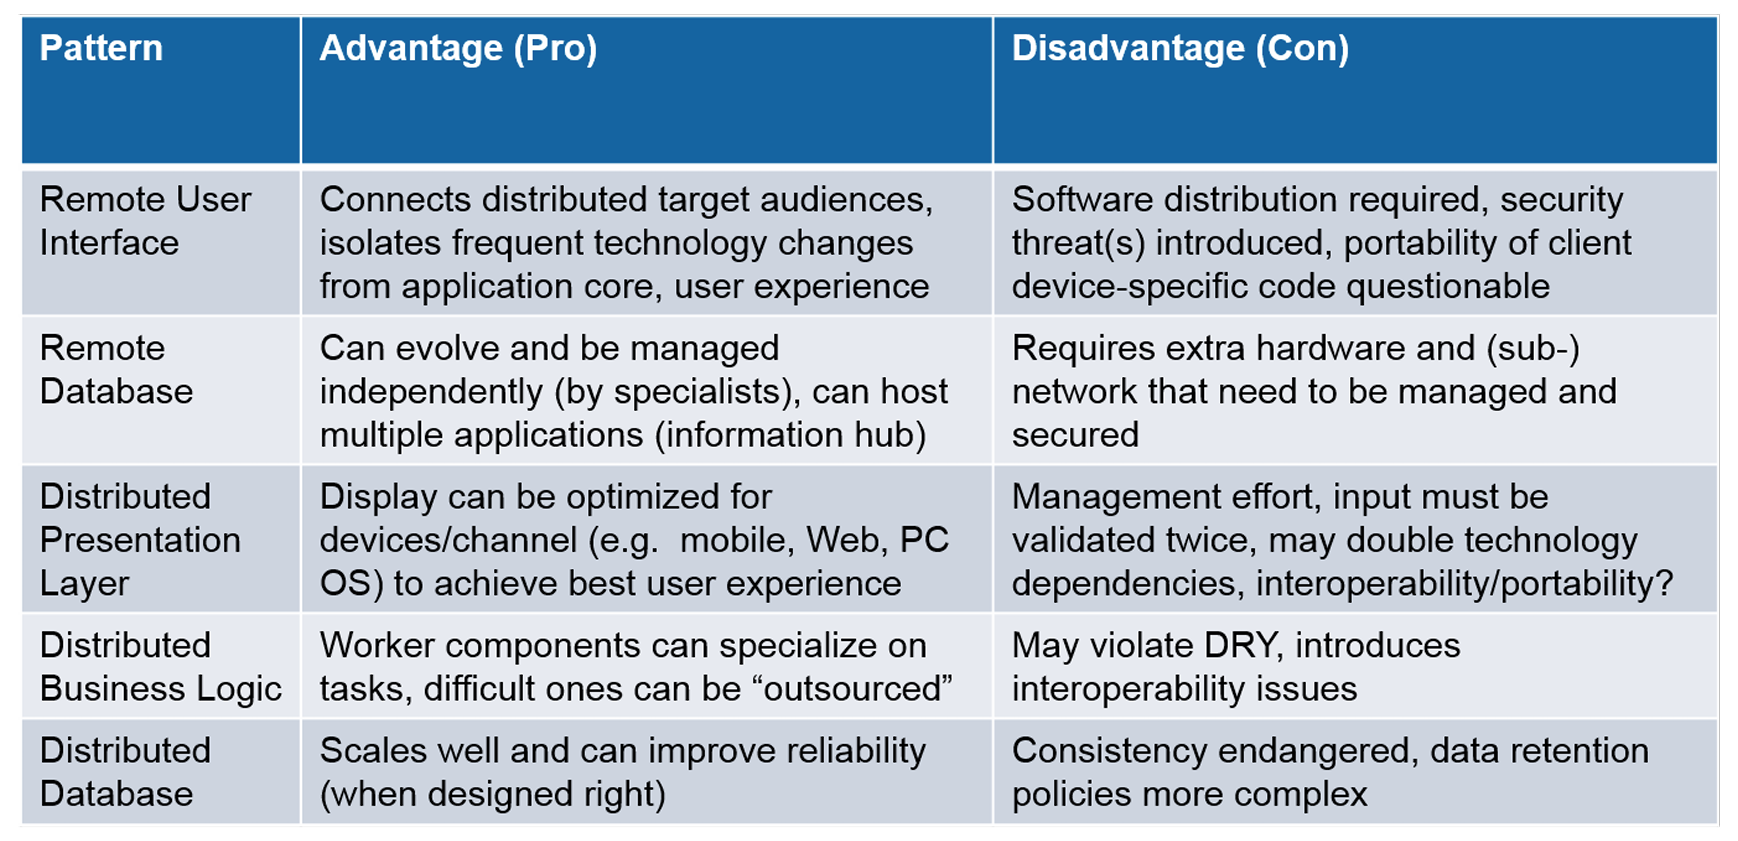
\includegraphics[width=1\linewidth]{Images/csc-pro-con.png}
    \caption{CSC Pro and Cons}
\end{figure}

\subsection{Container}
\defn{Container}{
    Container are \textbf{application-level frameworks} for tier 2 of a 2-tier or 3-tier
    application. Application level containers are not to be confused with container-based
    applications on the os system level. (ZIO)
}

In the \textbf{C4 model}, a container represents an application or a data store.
A container is something that needs to be running in order for the overall software system to work.
It is essentially a \textbf{runtime boundary} around some code that is
being executed or some data that is being stored.

\subsection{Container Architecture Patterns}
\textbf{Inversion of Control (IoC)} enables (container) frameworks to control server-side execution
and achieve extensibility with custom components even without recompilation.
With this pattern, a framework (or software component) \textbf{has control and manages the application component instances}.
The components know the interfaces of their members.
External requests arrive at the framework which redispatches them.

The overall goal is to enable high configuration flexibility
which leads to beeing able to swap implementations in and out which
is good for:
\begin{itemize}
    \item DevOps automation, CI/CD
    \item Running parallel versions
    \item Mocking
    \item Cloud vs inhouse deployment
\end{itemize}

\begin{figure}[H]
    \centering
    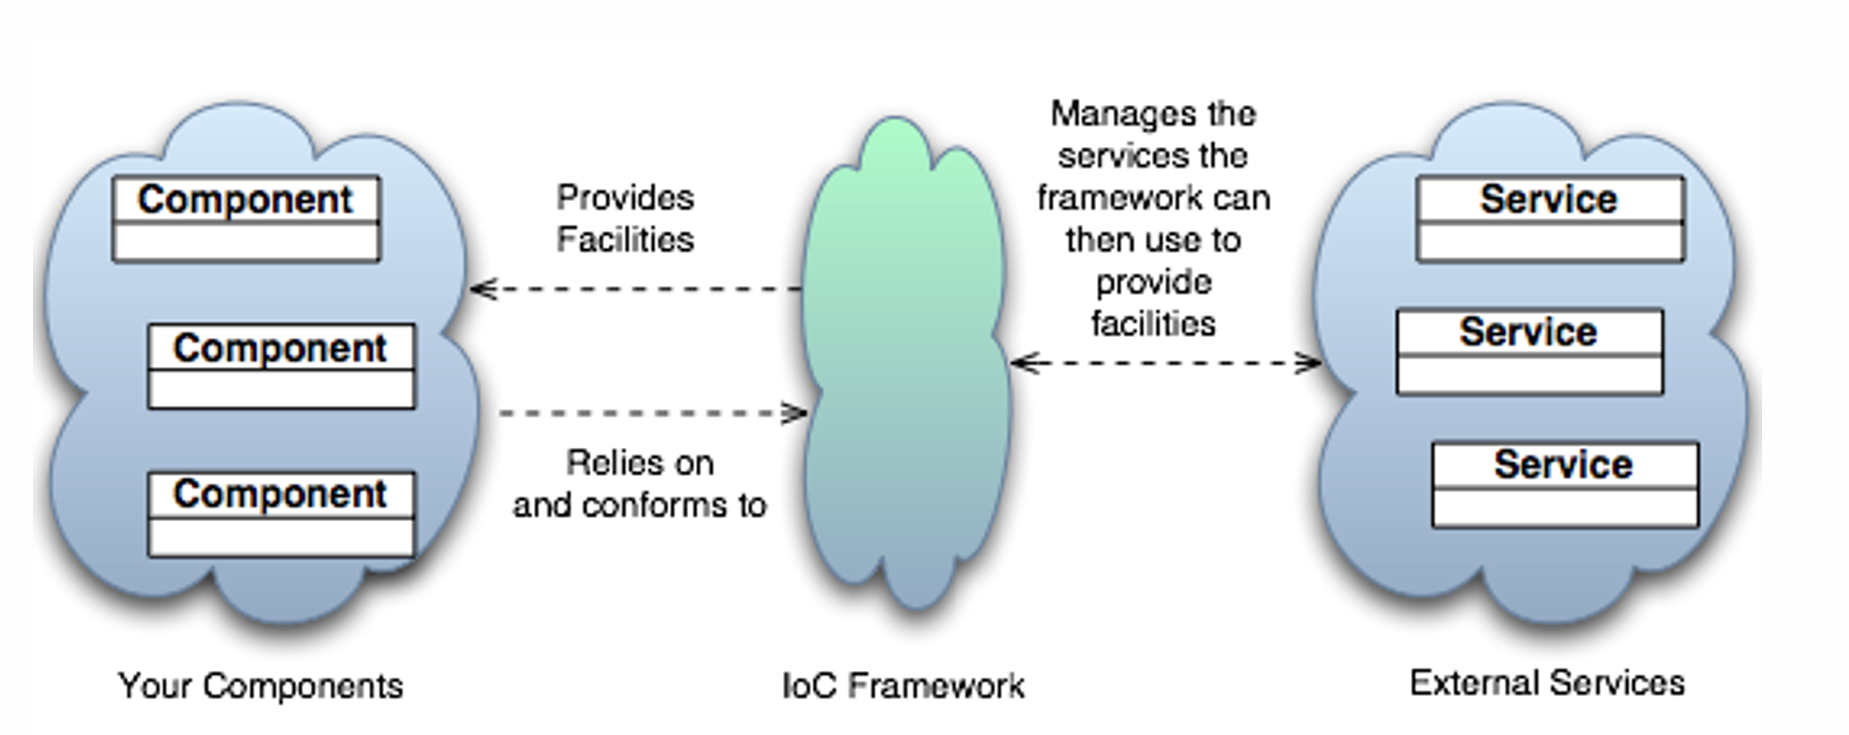
\includegraphics[width=1\linewidth]{Images/ioc.png}
    \caption{Inversion of Control}
\end{figure}

Interface implementations are received using \textbf{dependency injections}.
Which is a pattern that gives an object its instance variables.
This is good for isolating classes during testing and for systems
with many configurations. It is a one-step class member initialization.

\begin{figure}[H]
    \centering
    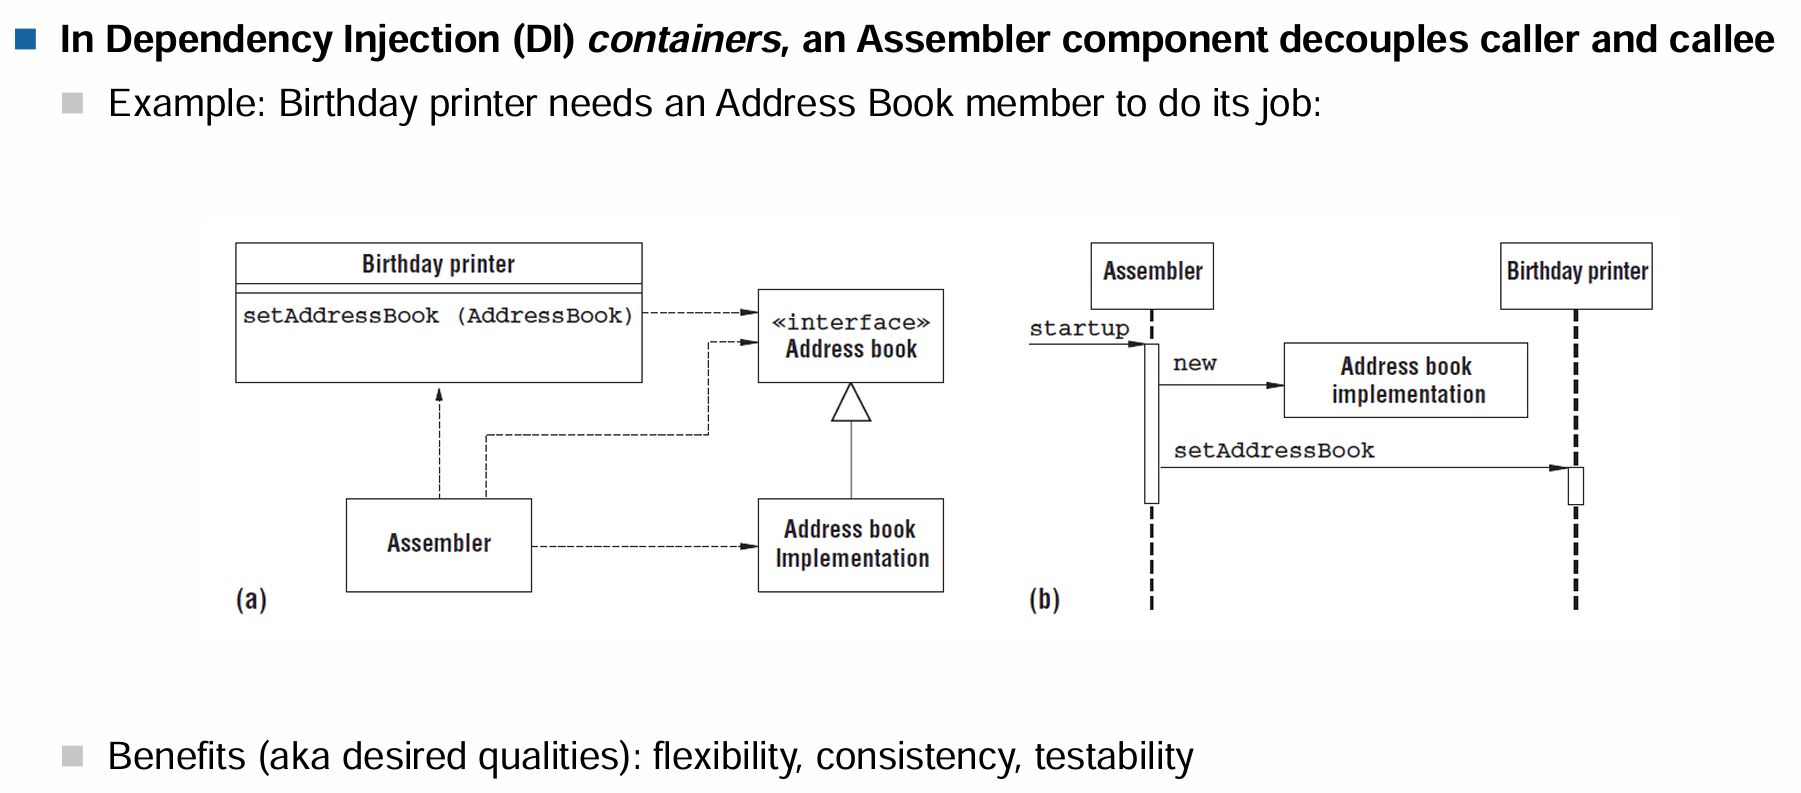
\includegraphics[width=1\linewidth]{Images/dep-injection.png}
    \caption{Dependency Injection}
\end{figure}

\subsection{Server-Side Container Architecture (Spring Boot)}

\begin{figure}[H]
    \centering
    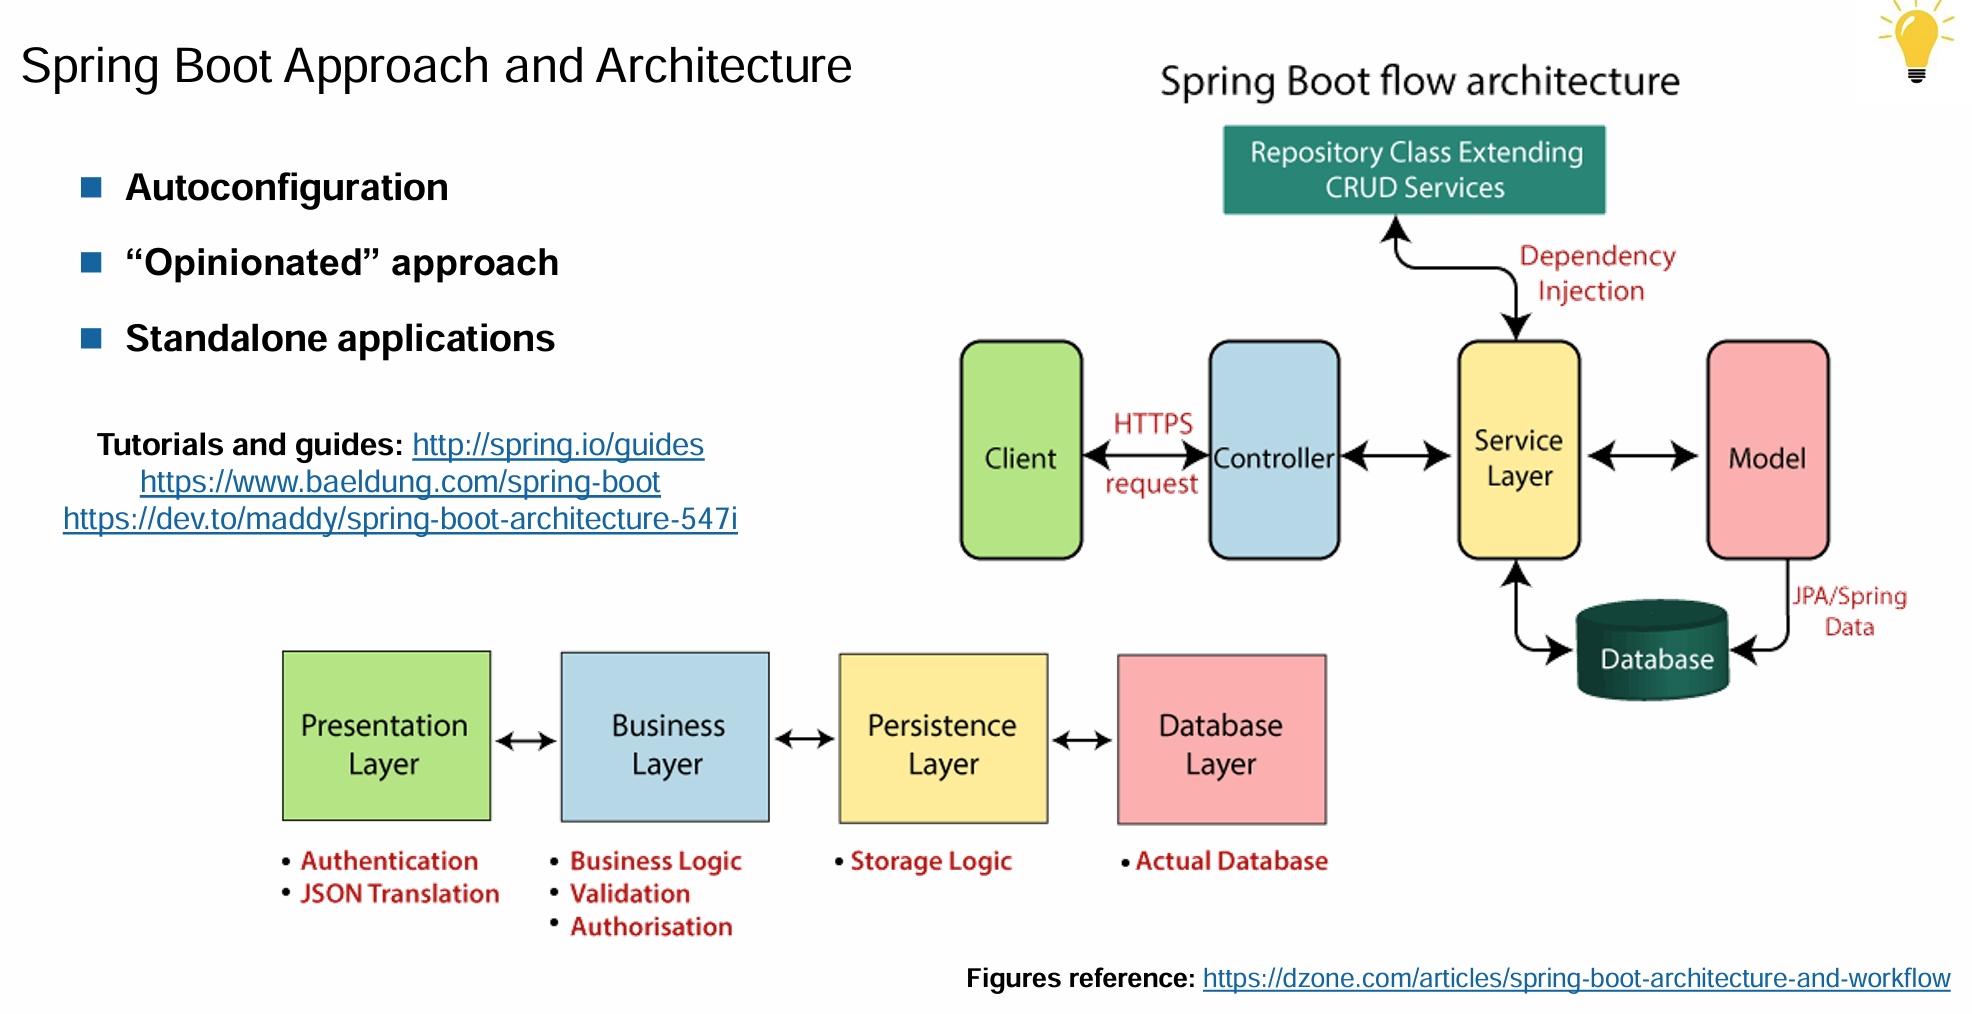
\includegraphics[width=1\linewidth]{Images/spring-boot-arch.png}
    \caption{Spring Boots Architecture Overview}
\end{figure}

\begin{figure}[H]
    \centering
    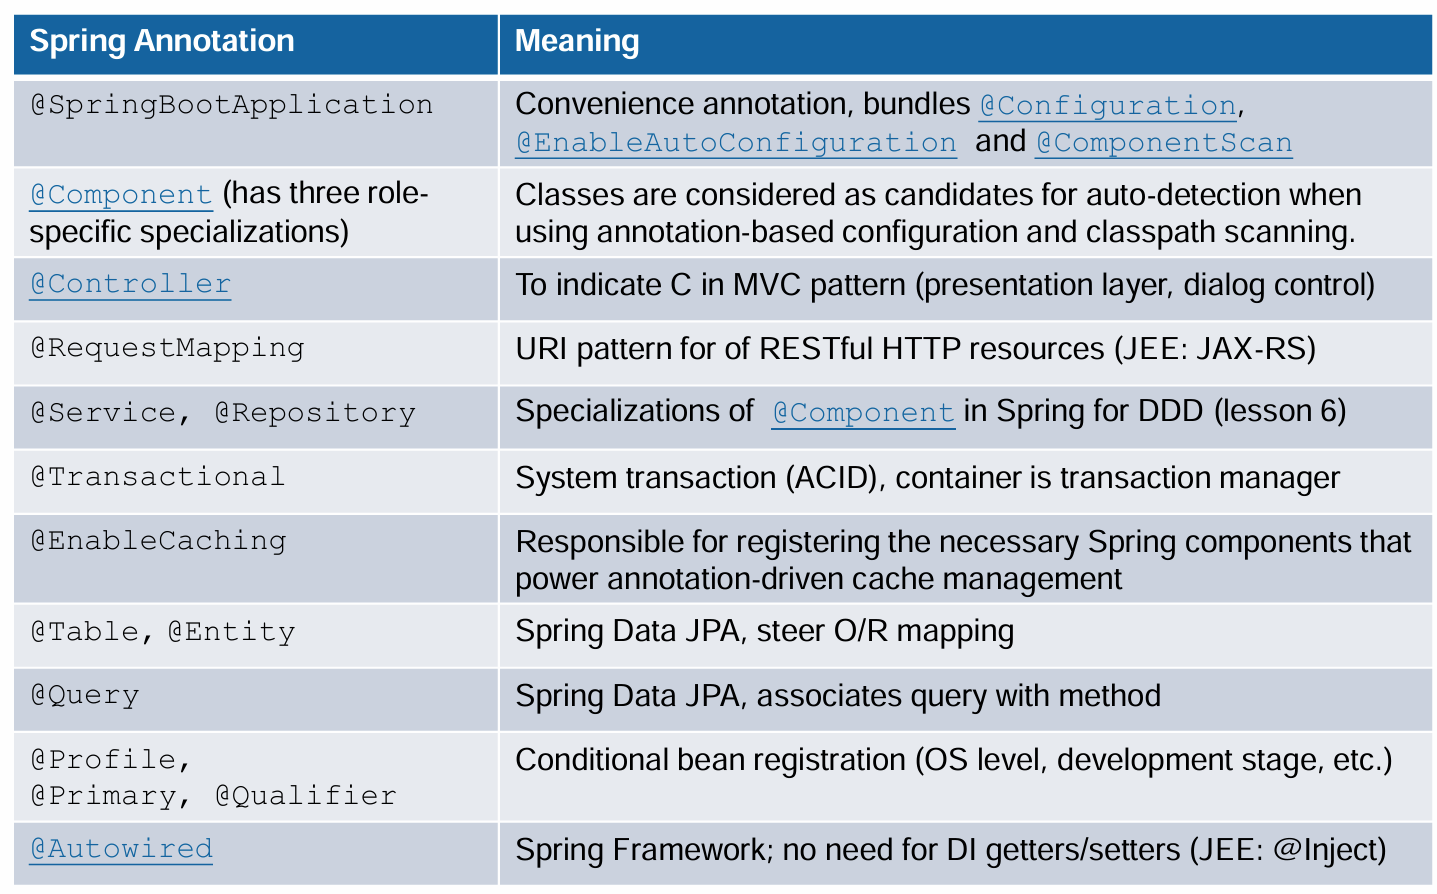
\includegraphics[width=1\linewidth]{Images/spring-boot-annotations.png}
    \caption{Key Spring Annotations}
\end{figure}

\subsection{Components}
\defn{Components}{
    A component is a grouping of related functionality encapsulated behind a
    well-defined interface. If you're using a language like Java or C\#,
    the simplest way to think of a component is that it's a collection of
    implementation classes behind an interface.
    \href{https://c4model.com/abstractions/component}{C4}
}
\exm{Components in C4}{
    With the C4 model, components are \textbf{not separately deployable units}.
    Instead, it's the container that's the deployable unit. In other words,
    all components inside a container execute in the \textbf{same process space}.
    Aspects such as how components are packaged (e.g. one component vs
    many components per JAR file, DLL, shared library, etc) is an
    orthogonal concern.
}
The components that we deal with in solution strategy are \textbf{candidate components}.
A candidate component is an intermediate/preliminary architectural element
used for planning, decision making, architectural prototyping.
The candidate components are subject to continuous refinement and
consolidation efforts (architectural refactoring).

\defn{Candidate Component (one Definition)}{
    A candidate component is an architectural element in the logical 
    viewpoint grouping related responsibilities that jointly satisfy
    one or more (non-)functional requirements so that design and
    implementation work can be planned and component realization
    decisions can be made.
}

\begin{figure}[H]
    \centering
    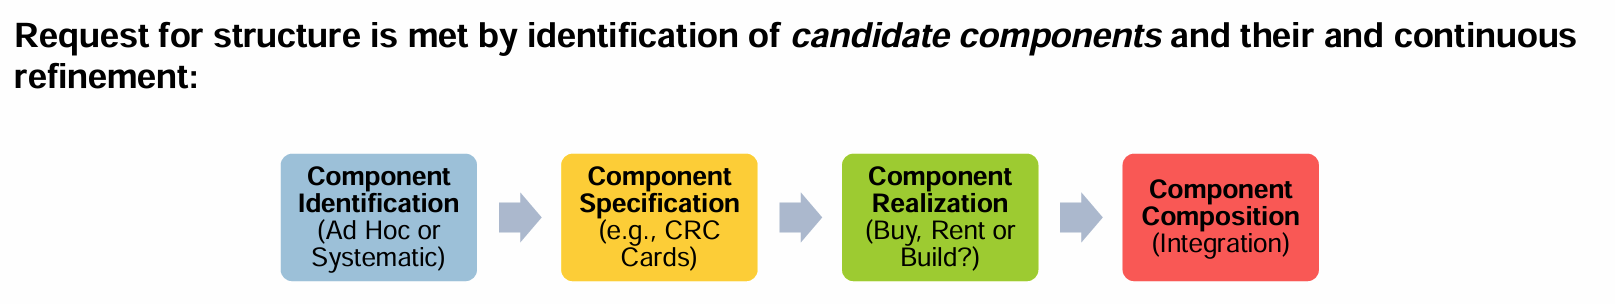
\includegraphics[width=1\linewidth]{Images/candidatecomponents.png}
    \caption{Candidate Components}
\end{figure}

Different stages of components can be identified during the whole creation of a software.
They should be created as candidate components during solution strategy, populated and refined into implementation
 components in project iterations. Deployment units then bundle one or more implementation components
to be hosted on one or more physical nodes (deployment viewpoint).

Other definitions depending on the viewpoint exist:
\begin{description}
    \item[Implementation]  reside in the development/implementation viewpoint. They group one 
    or more classes (in OOP) and provide an interface that hides their implementation details e.g. in 
    JEE and Spring. Their dependencies are made explicit and managed; they are versioned.
    \item[Deployment Units] then bundle one or more implementation components to be hosted on one or 
    more physical nodes (deployment viewpoint).
\end{description}

\newpage
\subsection{Component Interactions}
When modeling NFR with FURPS many design issues that also
concern dynamcs are yielded. Hence, architecture is not only
about structure, but also behaviour.
You should understand how (instances of) building blocks of
your system perform their job and communicate at runtime.
You will mainly capture scenarios in your documentation
to communicate your architecture to stakeholders that are
less willing or able to read and understand the static models
(building block view, deployment view). (ZIO)
More information with \href{http://docs.arc42.org/section-6/}{Runtime View on arch42}.

\begin{figure}[H]
    \centering
    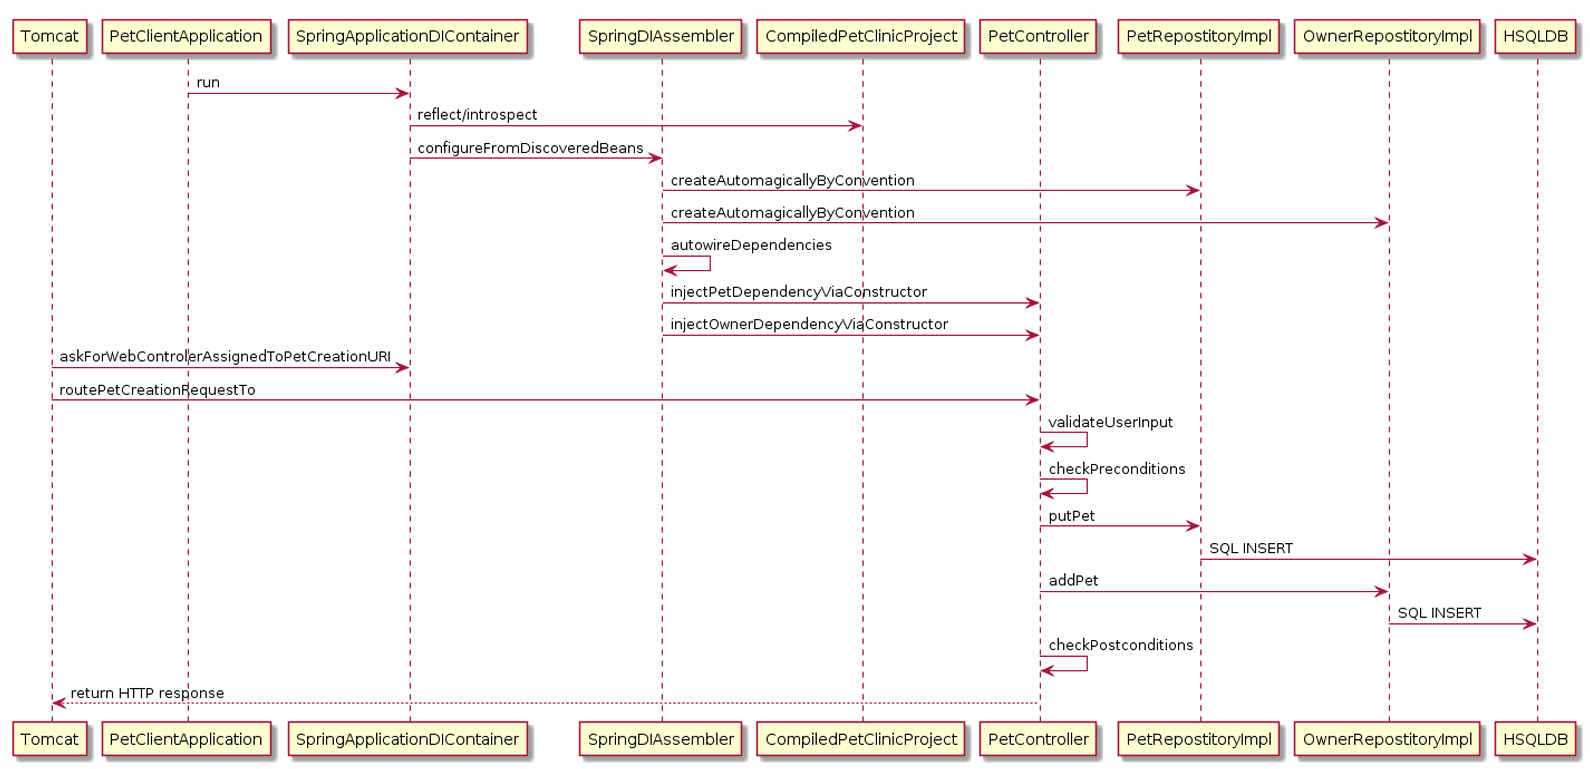
\includegraphics[width=1\linewidth]{Images/component-dynamics.png}
    \caption{Component Dynamics Example}
\end{figure}
\newpage

\newpage
\subsection{Common Components}
\begin{figure}[H]
    \centering
    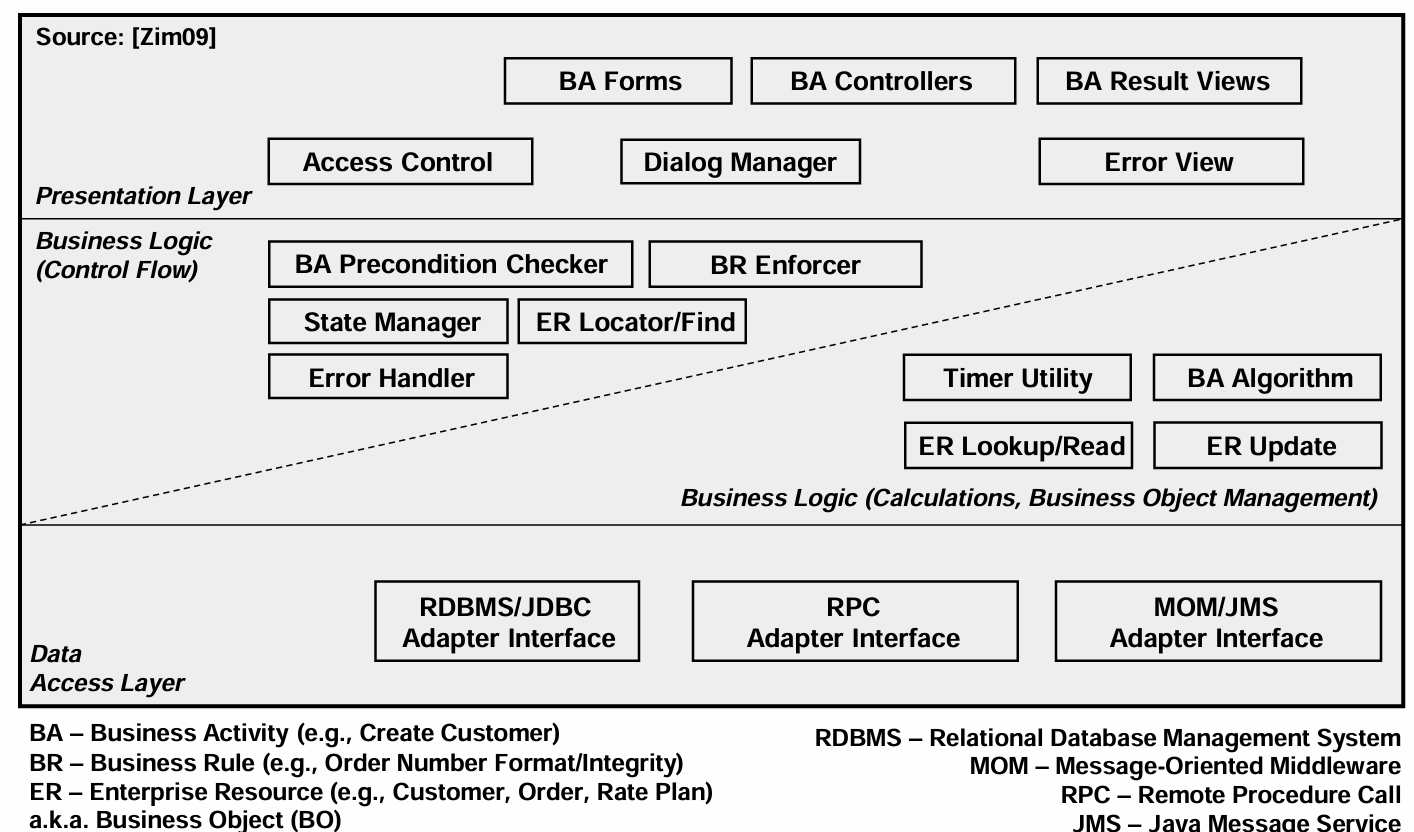
\includegraphics[angle=90,height=1.2\textwidth]{Images/commoncomponents.png}
    \caption{Common Components}
\end{figure}
\newpage

\subsection{Finding Candidate Components with Story Splitting (Agile Practice)}
Story that is too large for a sprint must be broken down to meet the \textbf{INVEST} properties of user stories.

\defn{INVEST Properties}{
    \begin{enumerate}
        \item Independent
        \item Negotiable
        \item Valuable
        \item Estimable
        \item Small
        \item Testable
    \end{enumerate}
}

\begin{figure}[H]
    \centering
    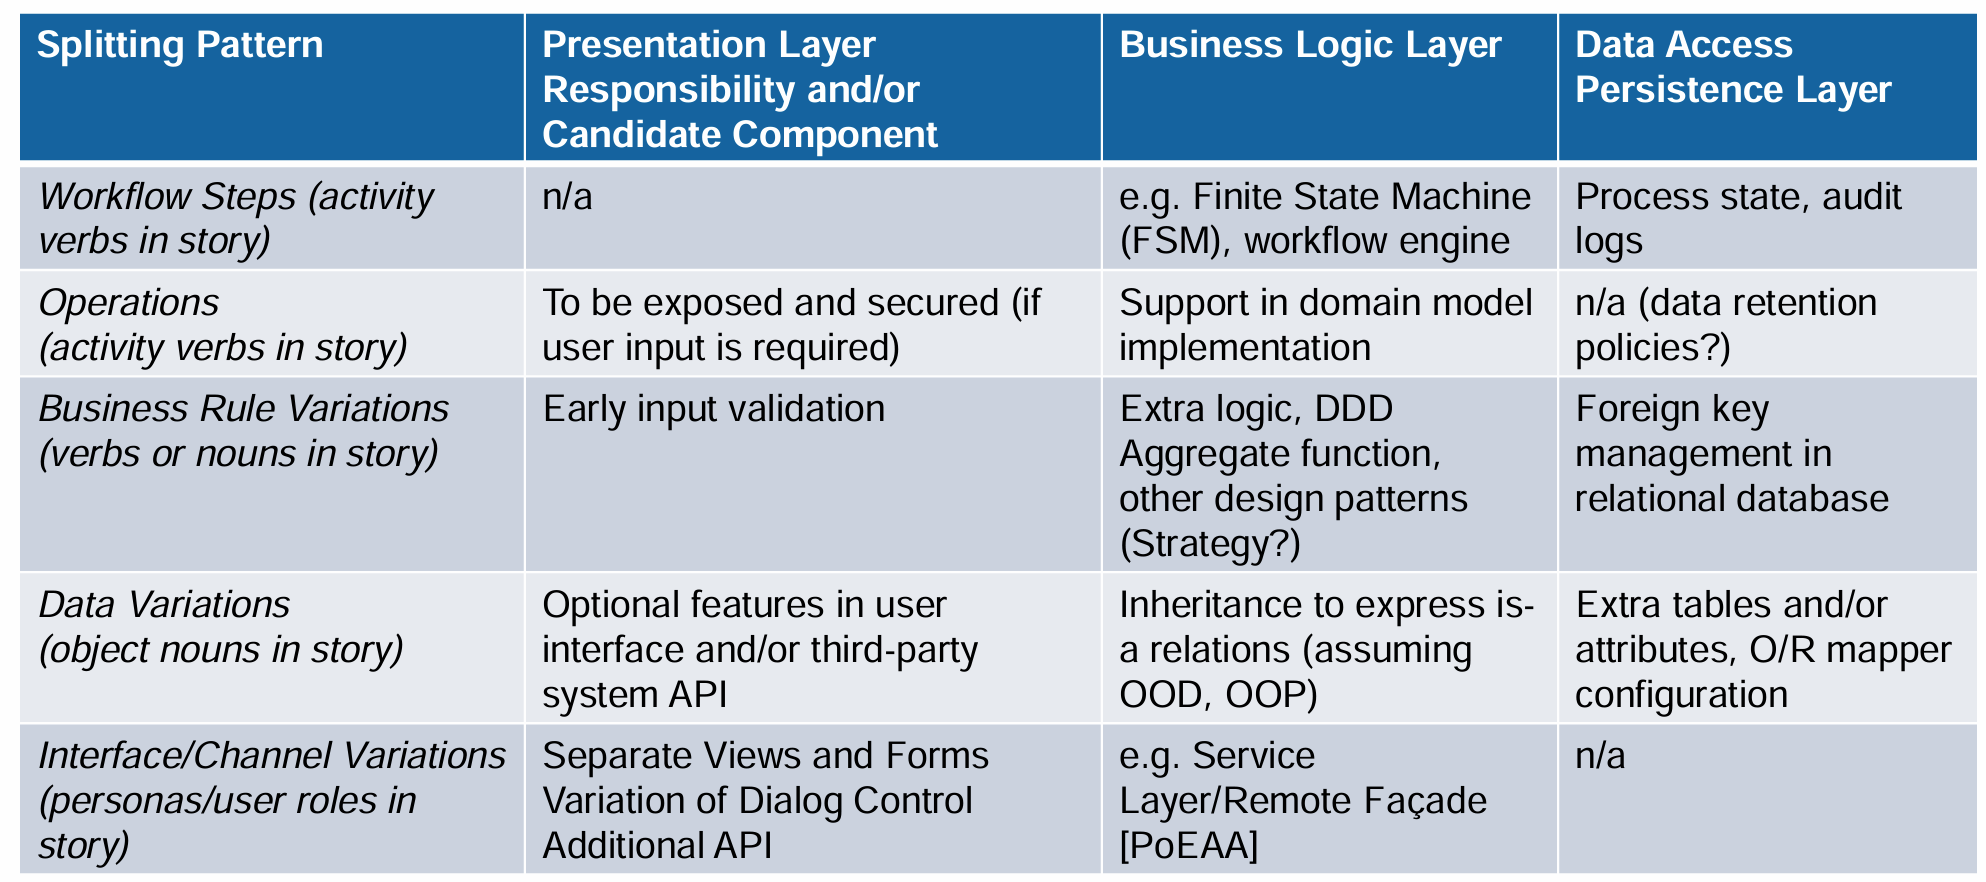
\includegraphics[width=1\linewidth]{Images/user-stories-components.png}
    \caption{User Stories for Components Example}
\end{figure}
\newpage
\begin{figure}[H]
    \centering
    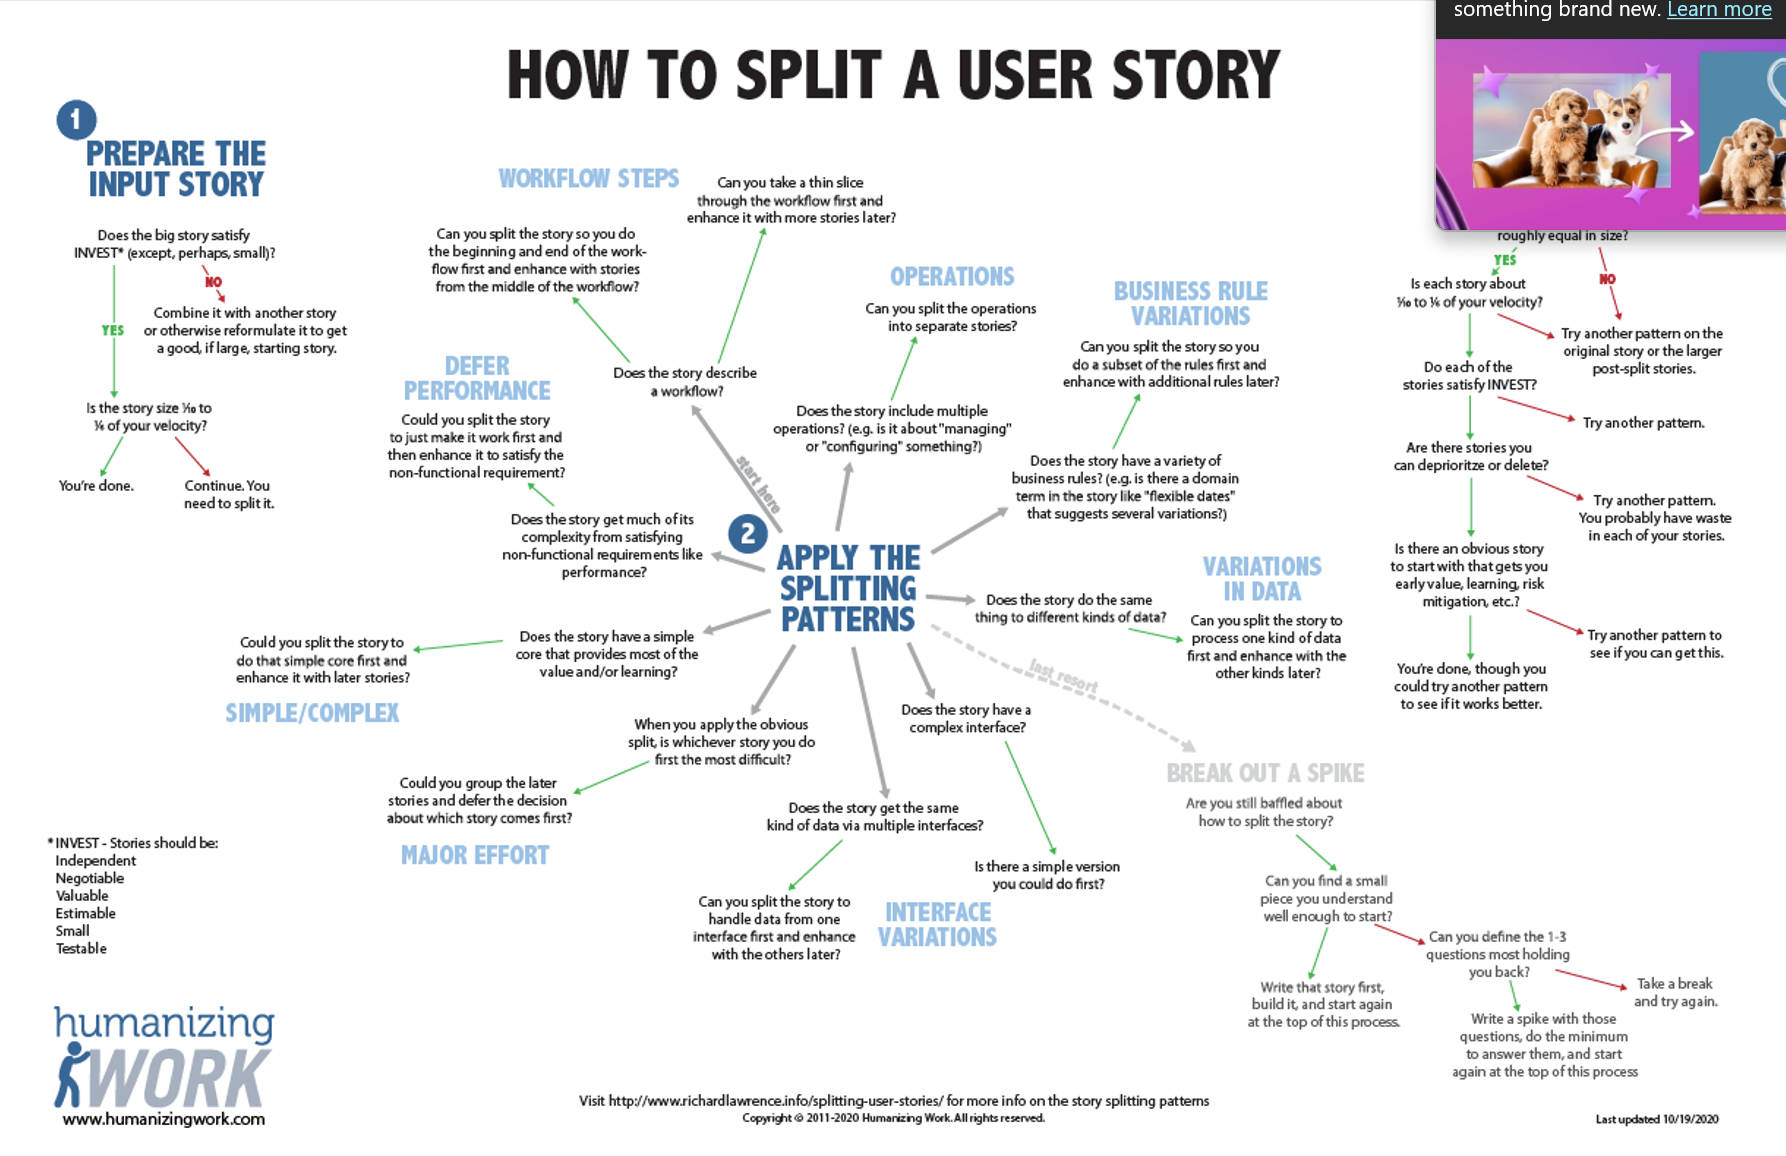
\includegraphics[angle=90,height=1\textwidth]{Images/storysplitting.png}
    \caption{Story Splitting Flowchart}
\end{figure}
\newpage

\begin{figure}[H]
    \centering
    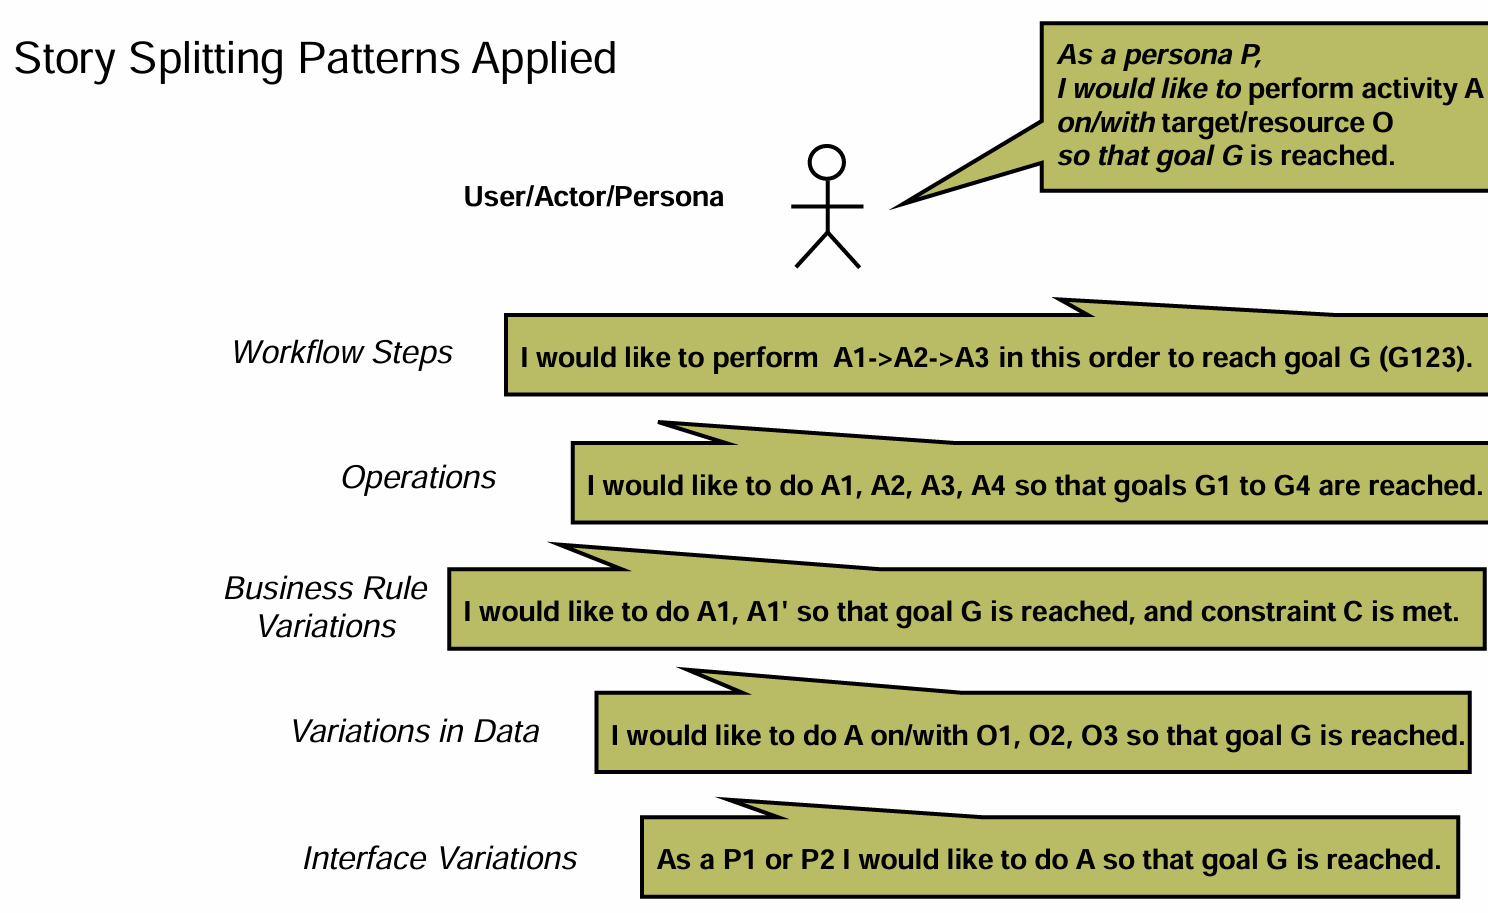
\includegraphics[width=1\linewidth]{Images/appliedstorysplitting.png}
    \caption{Story Splitting Example}
\end{figure}

\begin{table}
    \centering
    \begin{tabular}{|c|c|c|c|} \hline 
        Splitting Pattern&  Pres. Layer Responsibility &  Business Logic& Data Access Layer\\ \hline 
        Workflow Steps&  &  & \\ \hline 
        Operations&  &  & \\ \hline 
        Business Rule&  &  & \\ \hline 
        Data Variations&  &  & \\ \hline 
        Interface Variations& & &\\ \hline
    \end{tabular}
    \caption{Story Splitting Example Table}
\end{table}
\newpage

\subsection{Component Identification}
A rule of thumb is to \textbf{identify one candidate component per layer and
feature} or entity without knowing too much about them.
OOAD and business modeling techniques can help with CI.
There are many idefification techniques (e.g story splitting), but
we should always make a buy-rent-build decision for each candidate.
\defn{Commonly agreed/frequently listed criteria}{
    \begin{itemize}
        \item Partition by domain concepts (single responsibility principle)
        \item Partition by stakeholders or users (No reimplementations per user story (DRY!))
        \item Partition by product or data types (domain model entities)
        \item Add feature or component for locations and regions
        \item External interfaces to other systems
    \end{itemize}
    \href{https://web.archive.org/web/20201111235328/https:/techbeacon.com/app-dev-testing/practical-guide-user-story-splitting-agile-teams}{Mark Balbes}
}

\begin{figure}[H]
    \centering
    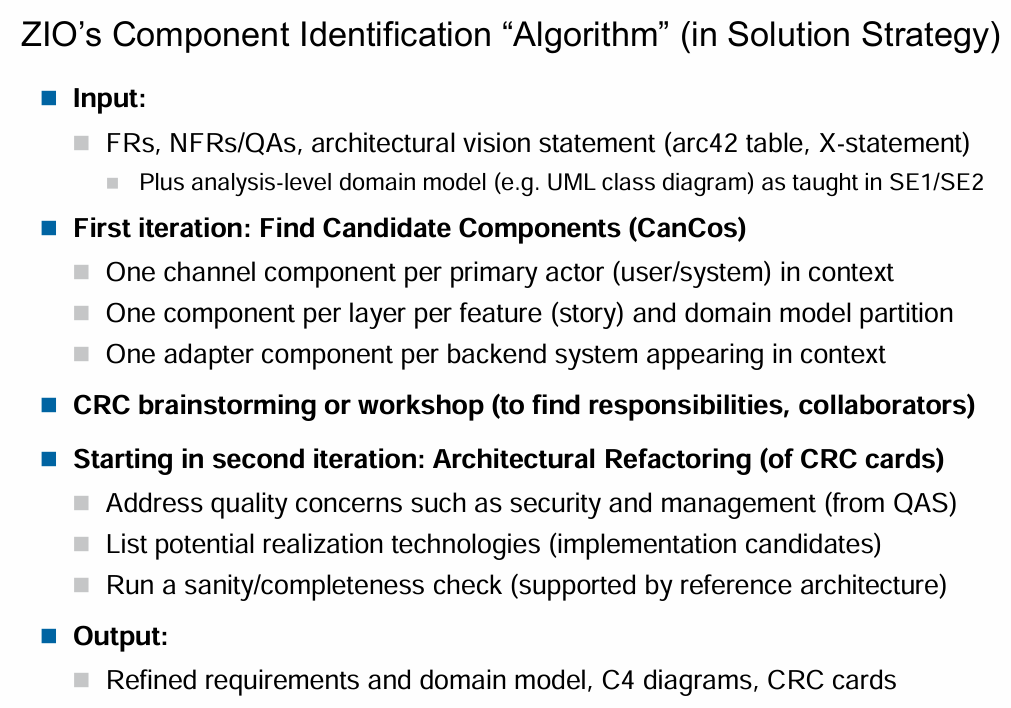
\includegraphics[width=1\linewidth]{Images/zio-idenfitication-algorithm.png}
    \caption{ZIO Component Identification Alorithm}
\end{figure}

\subsection{Components, Responsibilities, Collaborators (CRC) Cards}
The CRC card by W. Cunningham is a notation that is well suited for component modeling, 
complementing C4. CRC stands for Components, Responsibilities, Collaborators.
CRC must be expressive, but also easy to understand.
CRC cards can \textbf{complement component diagrams}.

\begin{figure}[H]
    \centering
    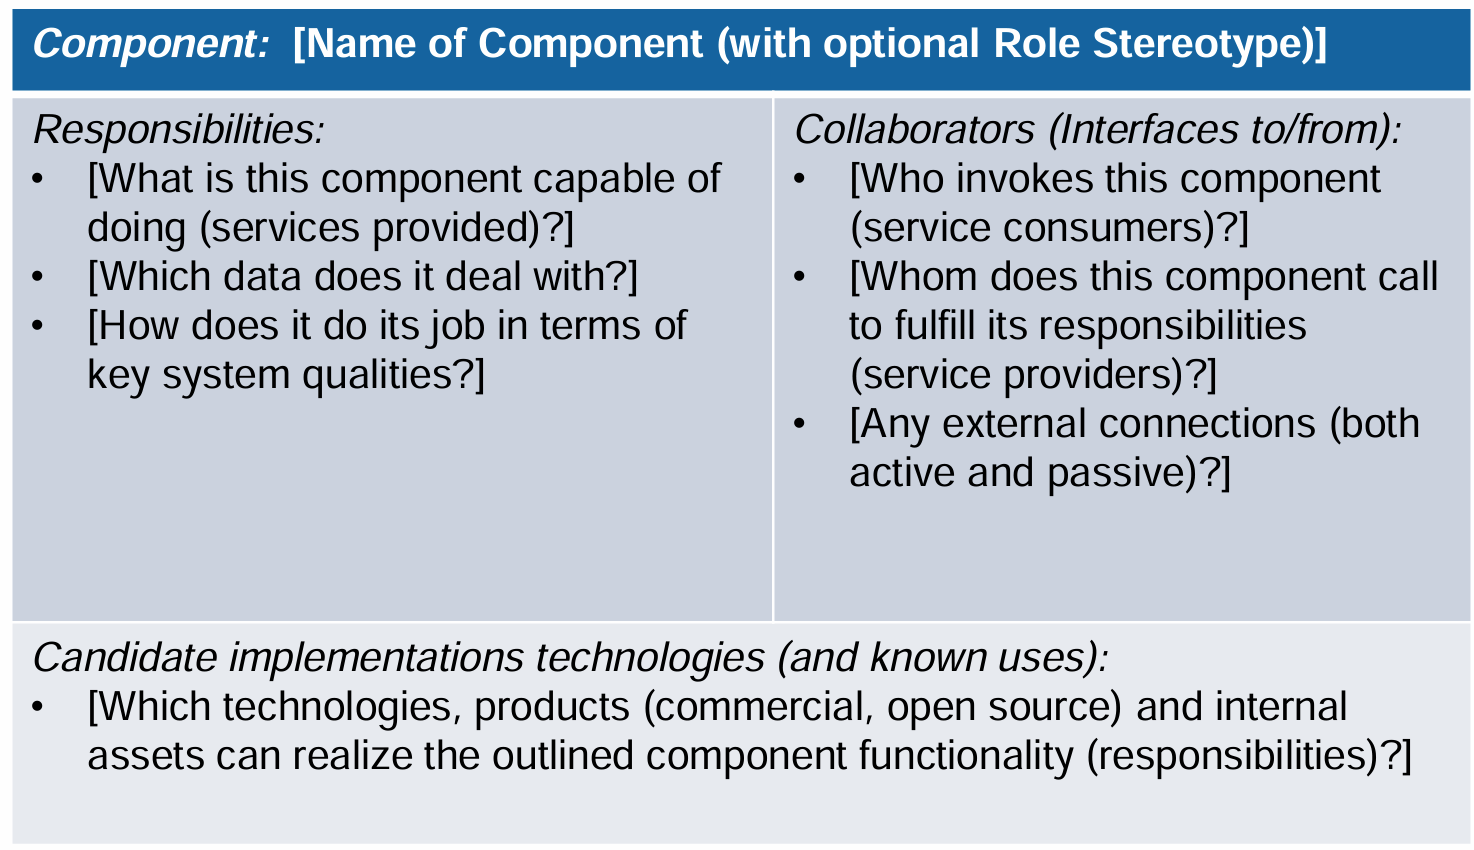
\includegraphics[width=1\linewidth]{Images/crc-card.png}
    \caption{CRC Card Template}
\end{figure}
\newpage

\section{Patterns of Enterprise Application Architecture (PoEAA)}
\defn{PoEAA}{
    The PoEAA book (Fowler 2002) is about the display, manipulation, and storage of large amounts of often complex data.
    \textbf{It only has one pattern called Domain Model to represent an object-oriented BLL},
    and describes Transaction Script (procedural) and Table Module (abstraction of Microsoft ADO Data Set Tools, COM/.NET) as alternatives.
}

The book is from 2003, the logical layers proposed and most base patterns are still valid.
Most patterns in PoEAA assume Distributed Presentation as CSC.
The Business Logic Layer patterns in the PoEAA book are rather simplistic (which is somewhat surprising) and
superseded and refined by Domain-Driven Design (DDD).
The well known patterns include:
\begin{itemize}
    \item MVC
    \item Template View
    \item Remote Facade (Integration)
    \item Data Transfer Object (DTO, Integration)
    \item Service Layer (refined in SOA and Microservices, Integration)
    \item Domain Model (refined by DDD)
\end{itemize}

\section{Domain Driven Design (DDD)}
DDD is a major software design concept introduced by the programmer Eric Evans in 2004, focusing on modelling
software to match a domain according to input from that domain’s expert. Properly applied it can lead to software
abstractions called domain models.
\defn{DDD}{
    \begin{description}
        \item[Tactic DDD] focuses on business logic in layered architecture models.
        It does so by decomposing the domain model pattern from Martin Fowler by introducing two
        BLL sublayers (application, domain).
        It emphasizes the need for modeling and communication in a ubiquitous language, the domain model.
        \item[Stategic DDD] emphasizes enterprise architecture and
        portfolio management. Boundaries are very important in a \textbf{macroscopic view}.
    \end{description}
}

\begin{figure}[H]
    \centering
    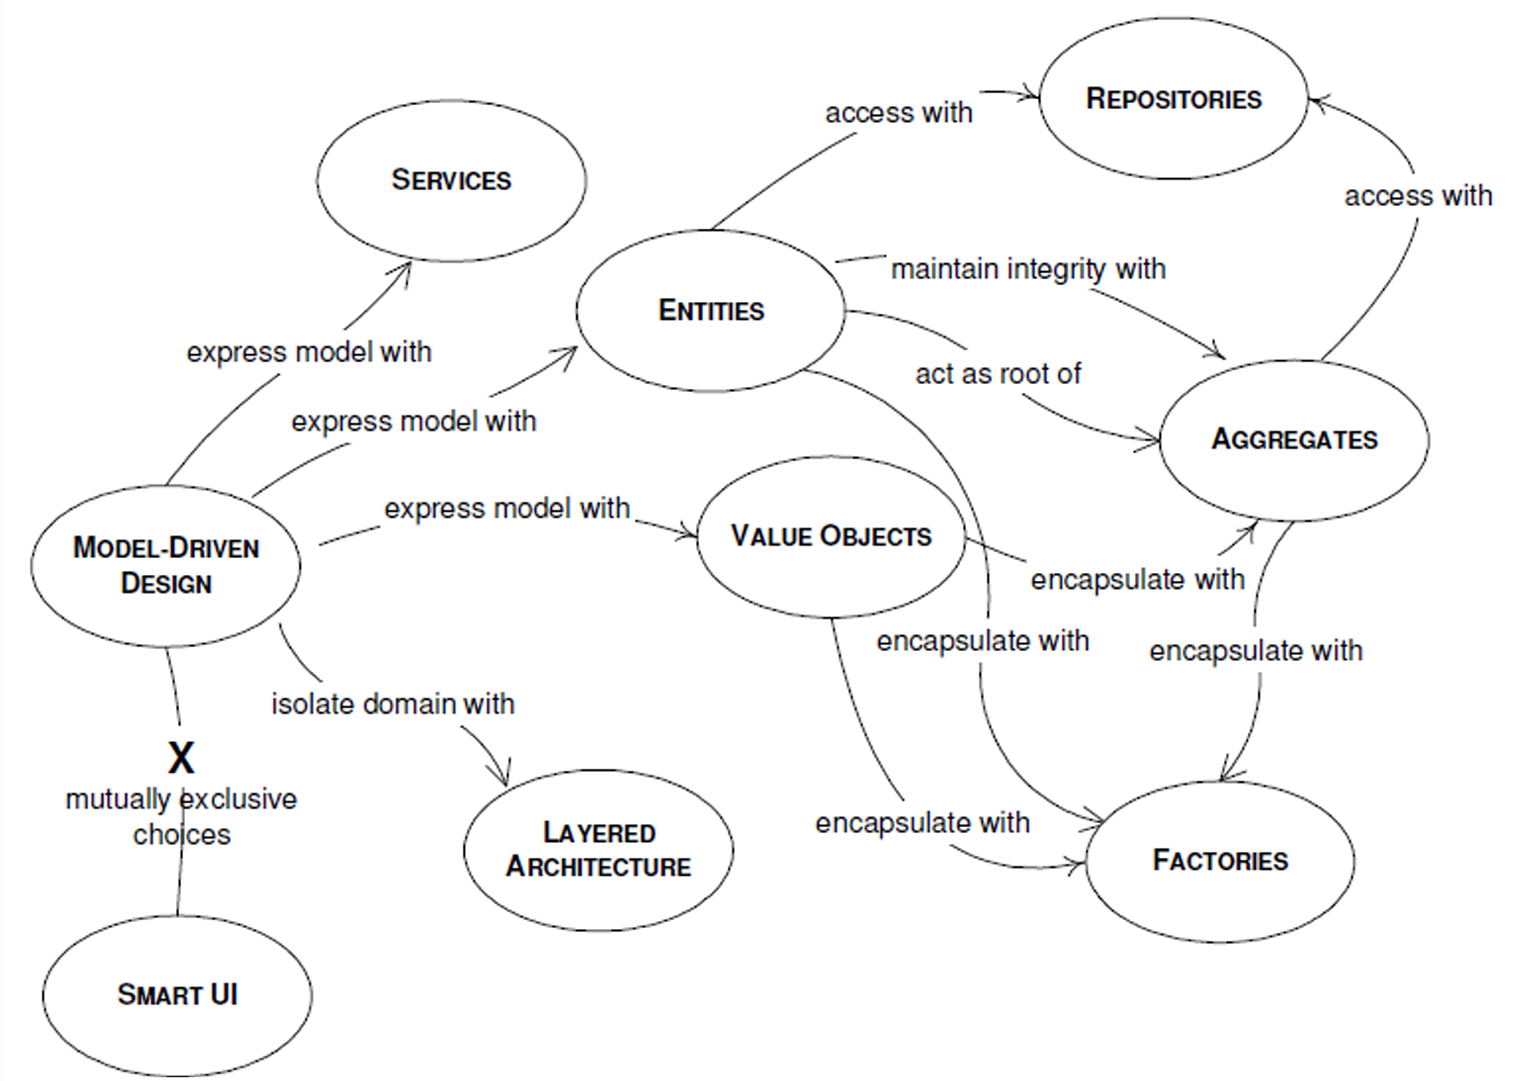
\includegraphics[width=0.8\linewidth]{Images/patternmap-tactic-ddd.png}
    \caption{Tactic DDD - Pattern Map}
\end{figure}

\newpage
\subsection{Tactic DDD and Logical Layers}
Layered Architecture pattern in DDD is not identical to PoEAA schema, but
it can be mapped in an easy way:
\begin{figure}[H]
    \centering
    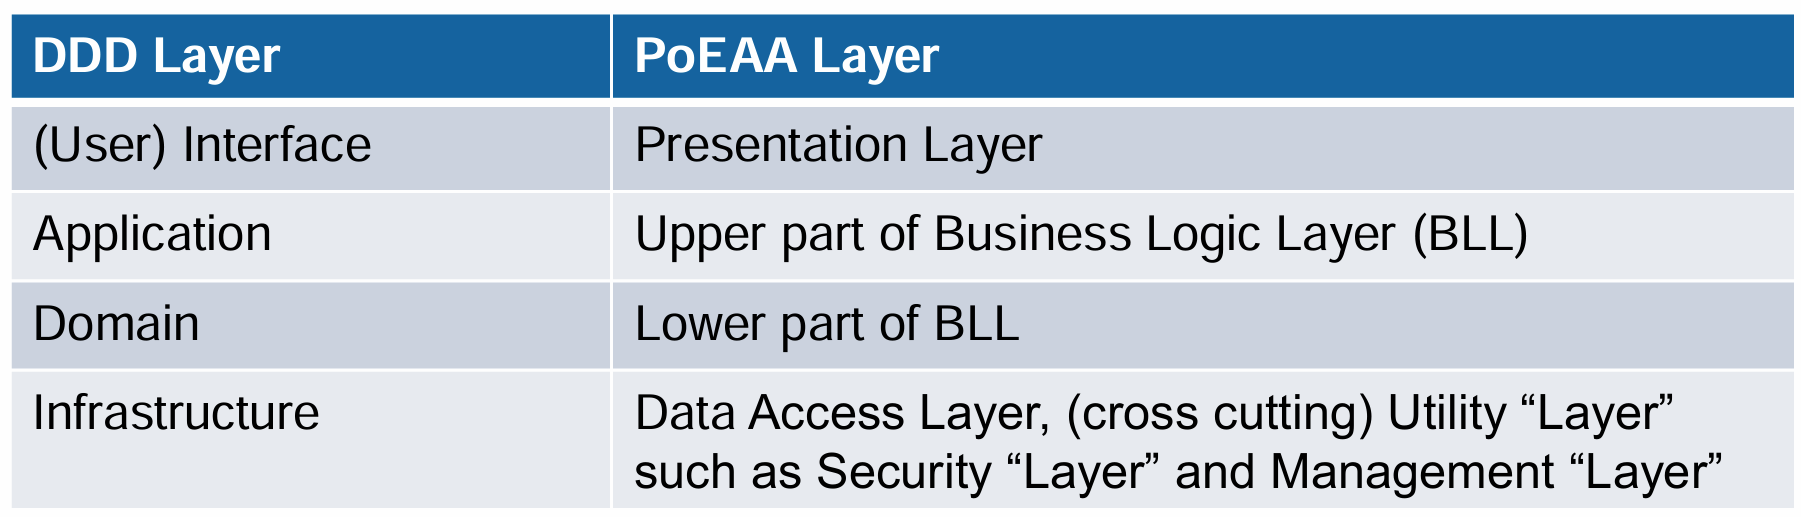
\includegraphics[width=1\linewidth]{Images/ddd-logical-layers.png}
    \caption{DDD and Logical Layers}
\end{figure}
The instances of tactic DDD primarily lives in the domain layer.
\begin{figure}[H]
    \centering
    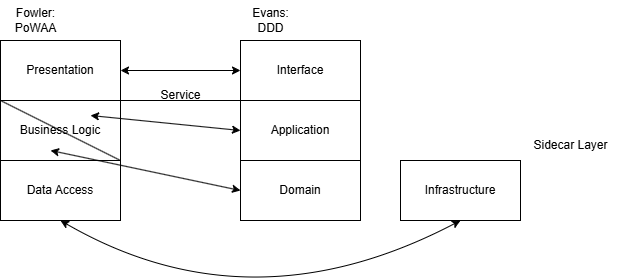
\includegraphics[width=1\linewidth]{Images/mapping-poeaa-ddd.png}
    \caption{Mapping PoEAA to DDD}
\end{figure}

\begin{figure}[H]
    \centering
    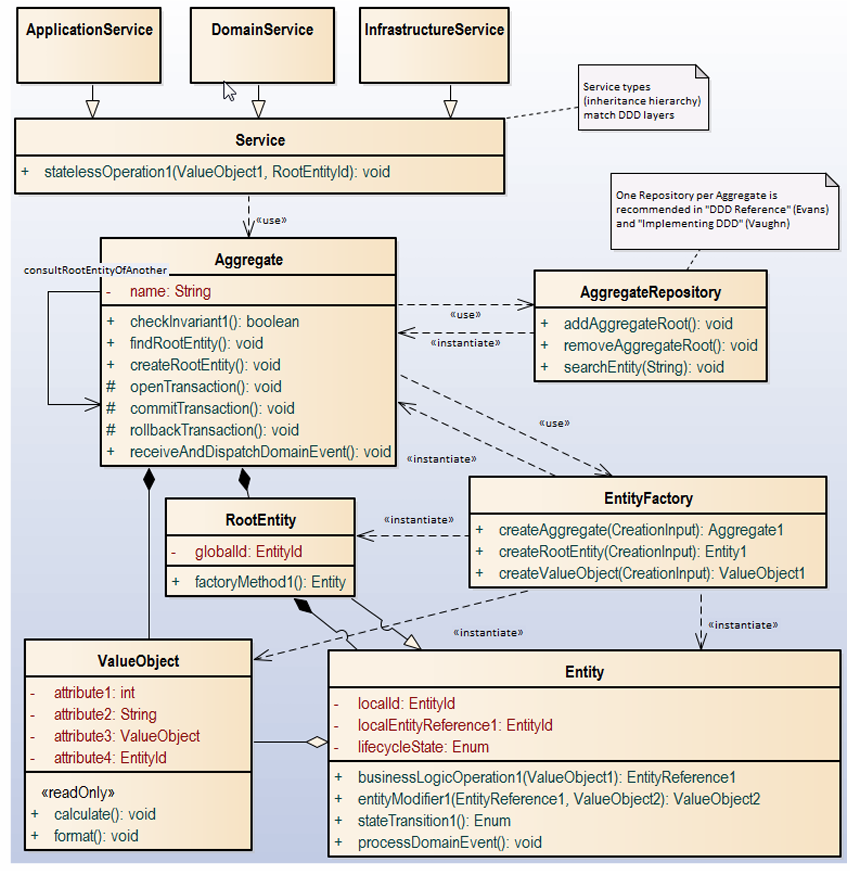
\includegraphics[width=0.75\linewidth]{Images/ddd-meta-model.png}
    \caption{DDD Domain Meta model}
\end{figure}
\newpage

\defn{Entity, Value, Aggregate}{
    \begin{description}
        \item[Entity] Entity is an object that has an \textbf{identifier and a lifecycle}.
        It can change states and can be distringuished by its identity
        and therefore is not defined by its attributes.
        \item[Value] The value object has \textbf{no identifier and is immutable}.
        Hence it has no state and is soely defined by its attribute.
        All operations on the value object must be side effect free.
        \item[Aggregate] An aggregate is a \textbf{collection (or graph) of entities and value objects}.
        It is the \textbf{smallest unit with functional consistency} while enforcing invariants.
        All objects of an aggregate are persisted toghether, this means
        the transaction boundary is around the collection.
        The aggregates has a root entity as external interface and entry point.
        External object should only reference the root entity.
        Aggregates are responsible for business rule enforcement accross entities.
    \end{description}  
}

\begin{figure}[H]
    \centering
    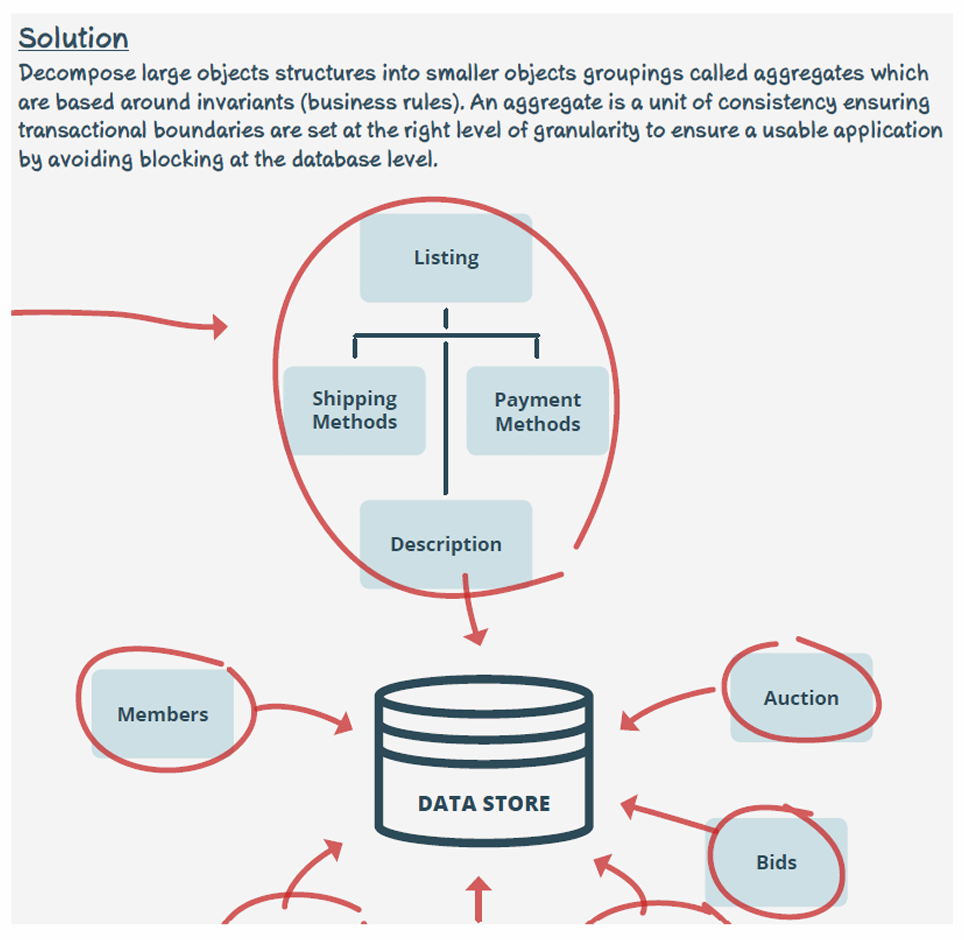
\includegraphics[width=0.75\linewidth]{Images/aggregate.png}
    \caption{Aggregate}
\end{figure}

\begin{figure}[H]
    \centering
    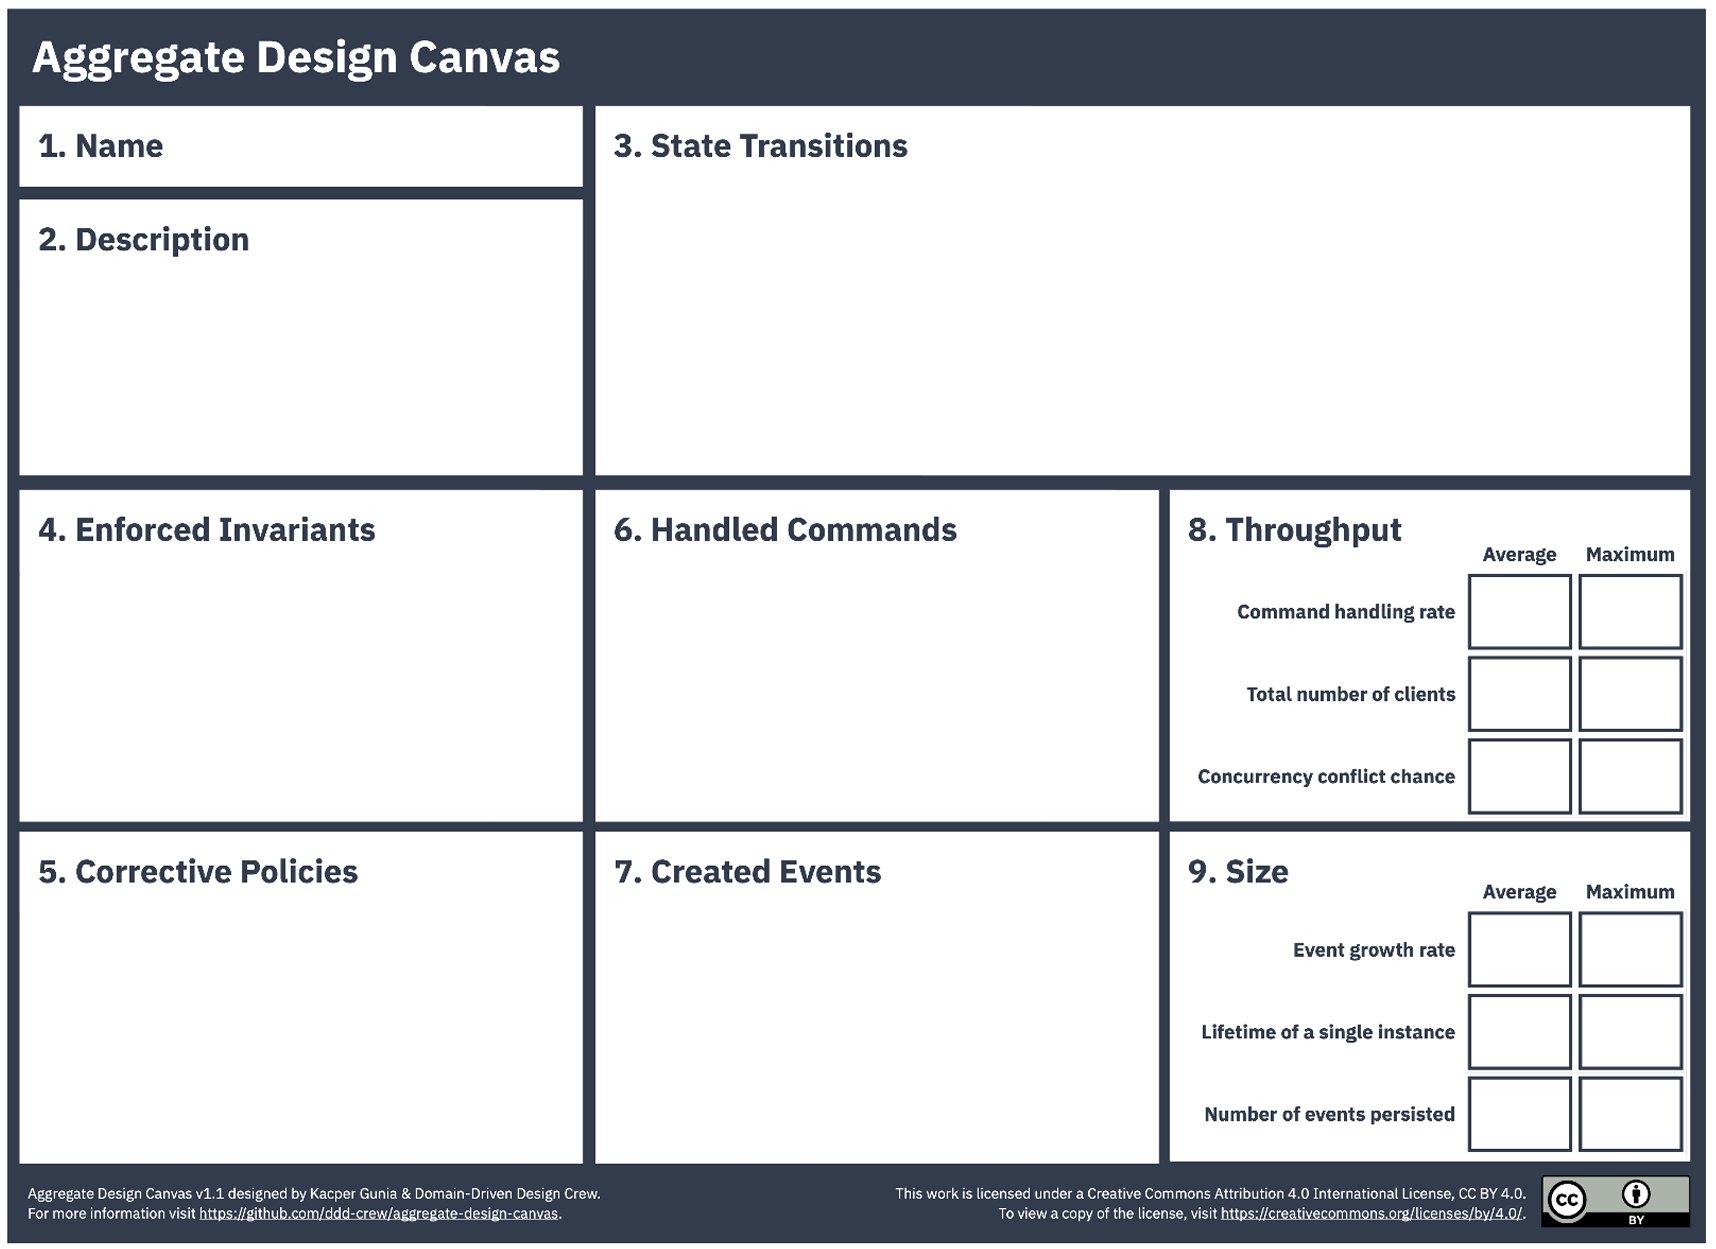
\includegraphics[width=1\linewidth]{Images/aggregate-design-canvas.png}
    \caption{Aggregate Design Canvas}
\end{figure}

\defn{Bussiness Rule and Invariants}{
    Business rule has (at least) two meanings:
    \begin{enumerate}
        \item Executable part of the business logic that is \textbf{not expressed as sequence} of statements, but \textbf{declaratively}.
        \item A \textbf{statement or condition} about the domain model, its elements and their relationship that \textbf{always has to be true} (invariant),
        to preserve data consistency and ensure accuracy of processing.
    \end{enumerate}
}
Examples of Invariants:
\begin{itemize}
    \item Physical containment relationship. (No order without an existing customer)
    \item Number calculations/value ranges (Total sum must not exceed value Y)
    \item Accounting and non-repudiation (All calls are billed)
\end{itemize}

\defn{Service}{
    A service exposes domain logic that crosses aggregate boundaries.
    Domain logic that cannot be assigned to a domain object naturally.
    The service is itself stateless and has several variants by sublayer:
    \begin{itemize}
        \item Domain services (core logic)
        \item Application services (not in domain model)
        \item Utility services
    \end{itemize}
}


\defn{Event}{
    An event is a representation of something that happened in the domain.
    Model activity is represented in the domain as a series of domain events.
    The events themselves are immutable. A domain event is always something
    that happened in the past, and since we cannot change the past, it is immutable.
    Events may be exchanged between aggregates.
}

\defn{Repository}{
    The repository is an entity that handles persistence of the aggregates.
    There may be one repository per aggregate and it interacts with the root entity.
    Repositories themselves do not contain business logic and only the interface
    belongs to the core domain model. This makes the implementation replaceable.
}


\subsection{Best-Practices}
\begin{itemize}
    \item Use asynchronous communication between aggregates
    \item Give enforcement responsibilities to root entity, possibly supported by designated framework mechanisms
    \item Keep one aggregate on one server, allow different aggregates to be distributed among hardware
    \item Use the same boundaries for transactions and distribution
    \item Model true invariants in consistency boundaries
    \item Design small aggregates
    \item Reference other aggregates by identity
    \item Use eventual consistency outside the boundary
\end{itemize}

\newpage

\subsection{OOA to Tactic DDD}
\begin{enumerate}
    \item Distinguish Entities (stateful) and value objects (stateless). Put non-OO code in services
    \item Group output of step 1 into aggregates (storage units). Let aggregates communicate state changes via domain events.
    \item Add a repository for each aggregate. One may also add factories.
\end{enumerate}
\newpage

\section{Strategic DDD}
\defn{Strategic (Macro) DDD}{
    Strategic Domain Driven Design is concerned with designing the domain
    model inside a bounded context.
}

It deals with integrating these components and managing complexity in end-to-end application landscapes for the long run.
In small projects and businesses such long-time perspective might be unneeded.
\\\\
DDD provides two abstractions for model partitioning, both supporting a divide-and-conquer approach to managing complexity.
They differ in their scope and viewpoint taken:
\begin{description}
    \item[Subdomain] functional
    \item[Bounded Context] Organizational and technical  
\end{description}

Four advantages of using model partitioning and context boundaries:
\begin{itemize}
    \item Same term, different meaning (homonym)
    \item Same concept, different different use (polyseme)
    \item External system differences (heterogeneity)
    \item Scaling up the organization (multiple teams)
\end{itemize}

\defn{Bounded Context (BC)}{
    Bounded Contexts are descriptions of a boundary within which a particular model
    is defined and applicable.
    Bounded contexts implement parts of one or multiple subdomains.
    Subdomains are specific problem spaces as a result of object oriented analysis.
    Bounded context are in the solution space and are a result of object oriented design.
}
Subdomain is a top-down approach whereas BC partitions in a bottom-up way.
DDD does not mandate any particular syntax such as UML, pattern icons or pictograms, hence you can visualize in different ways.

\begin{figure}[H]
    \centering
    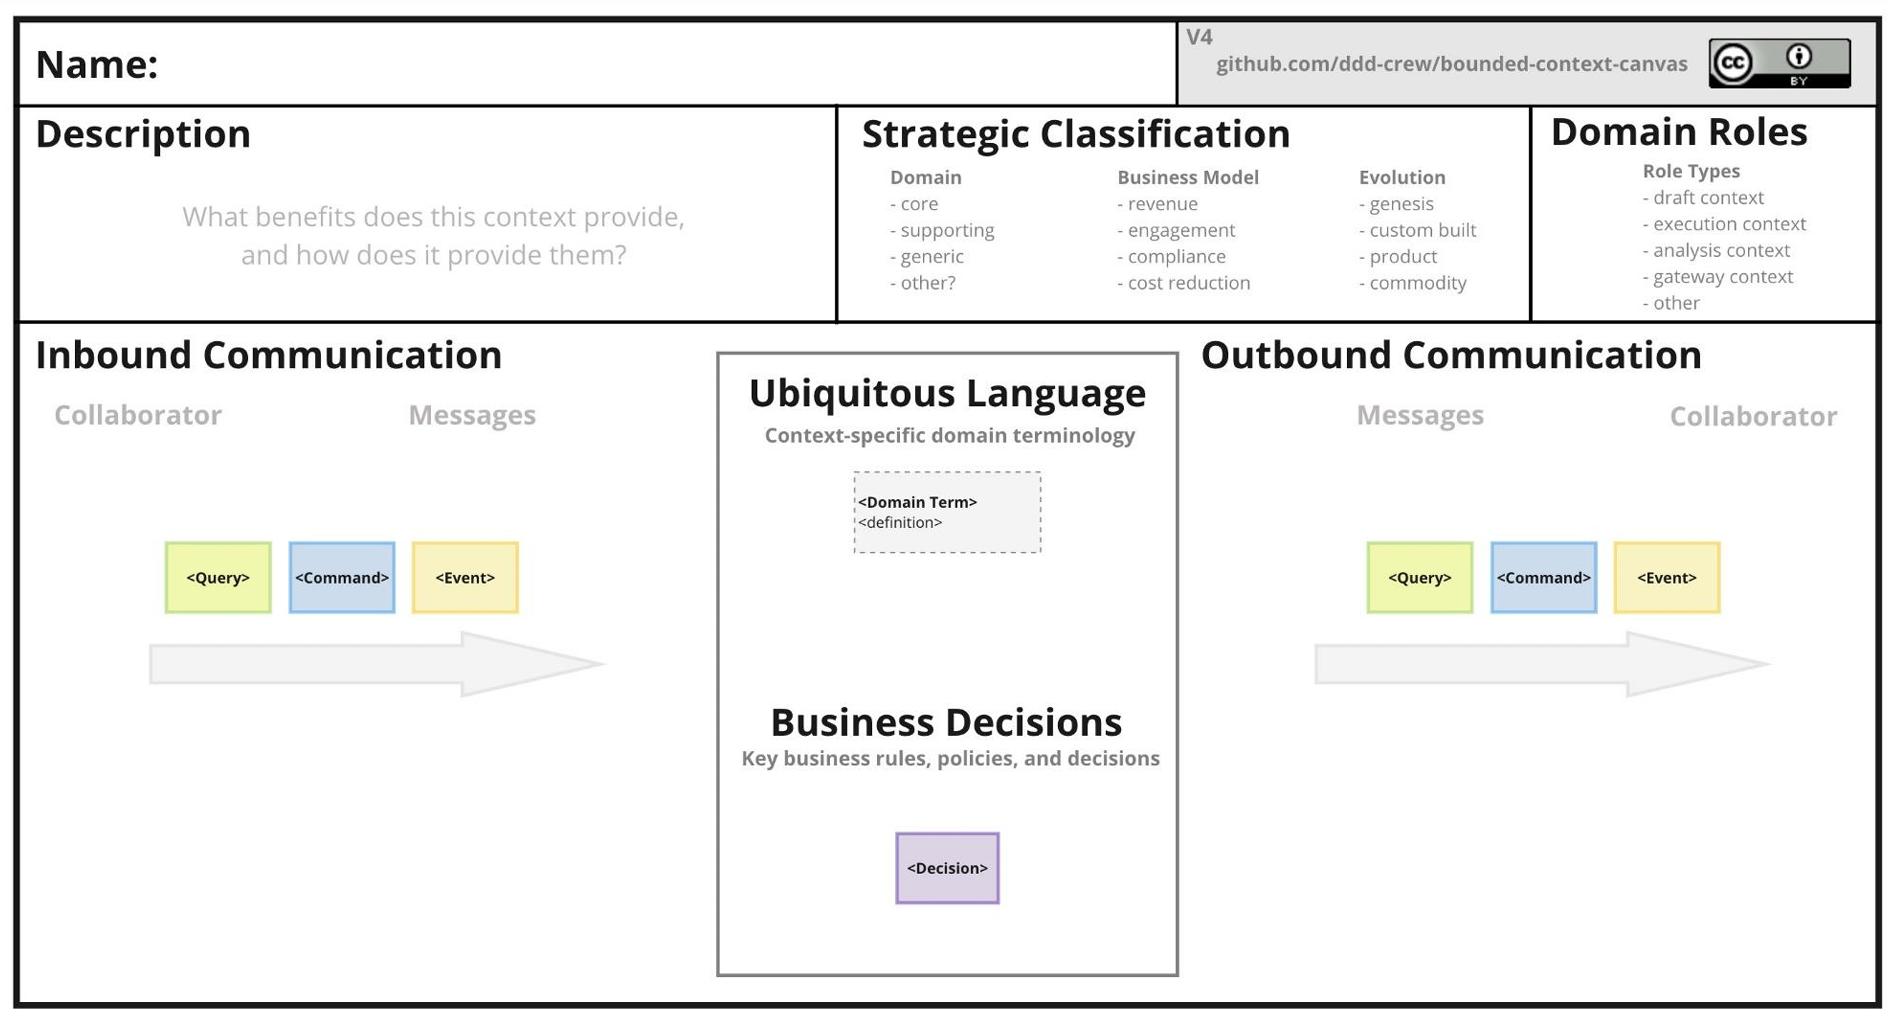
\includegraphics[width=1\linewidth]{Images/bounded-context-canvas.png}
    \caption{Bounded Context Canvas}
\end{figure}

\begin{figure}[H]
    \centering
    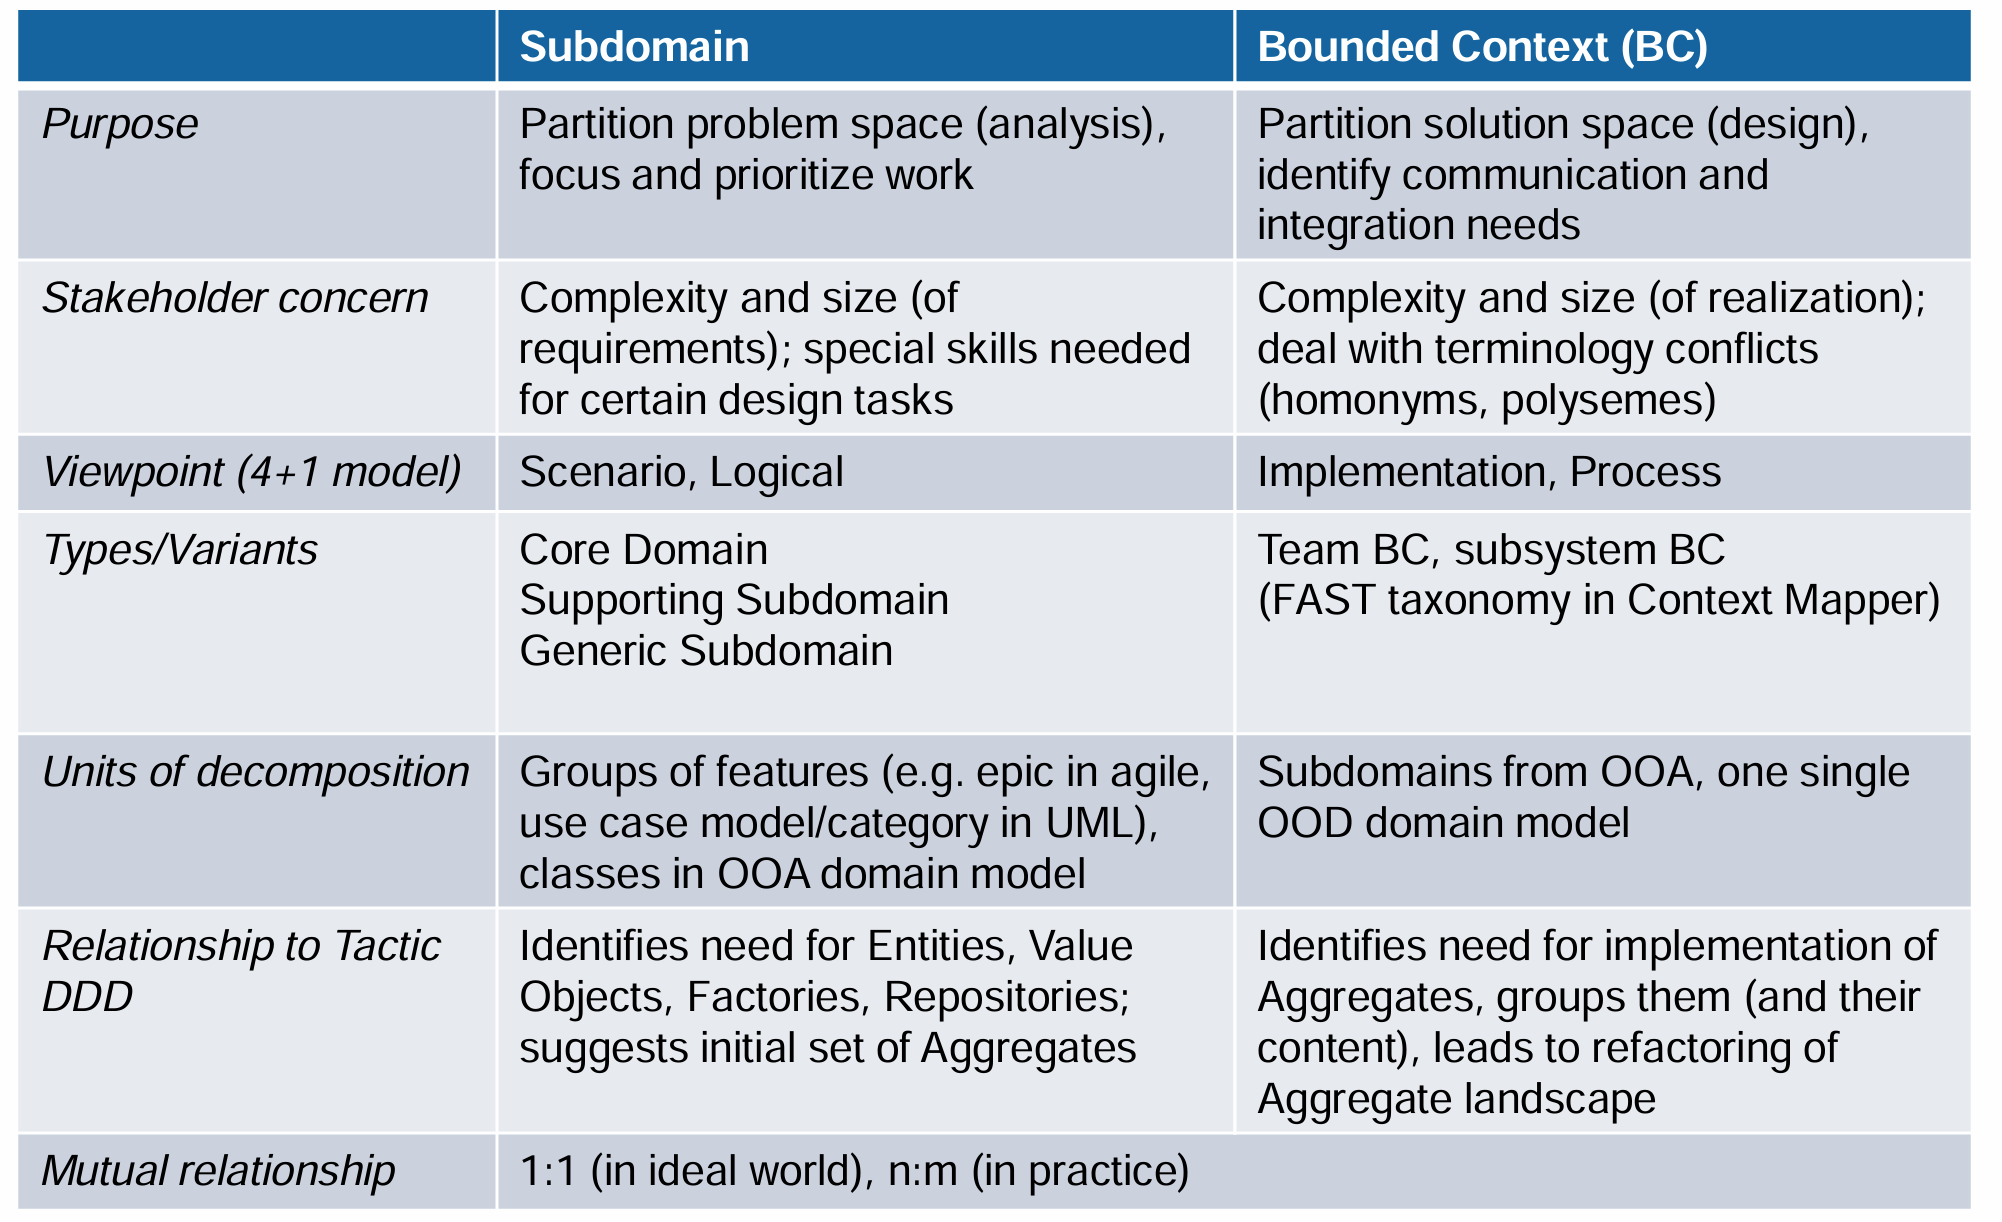
\includegraphics[width=1\linewidth]{Images/subdomain-vs-bc.png}
    \caption{Subdomains vs Bounded Context Comparison}
\end{figure}

\begin{figure}[H]
    \centering
    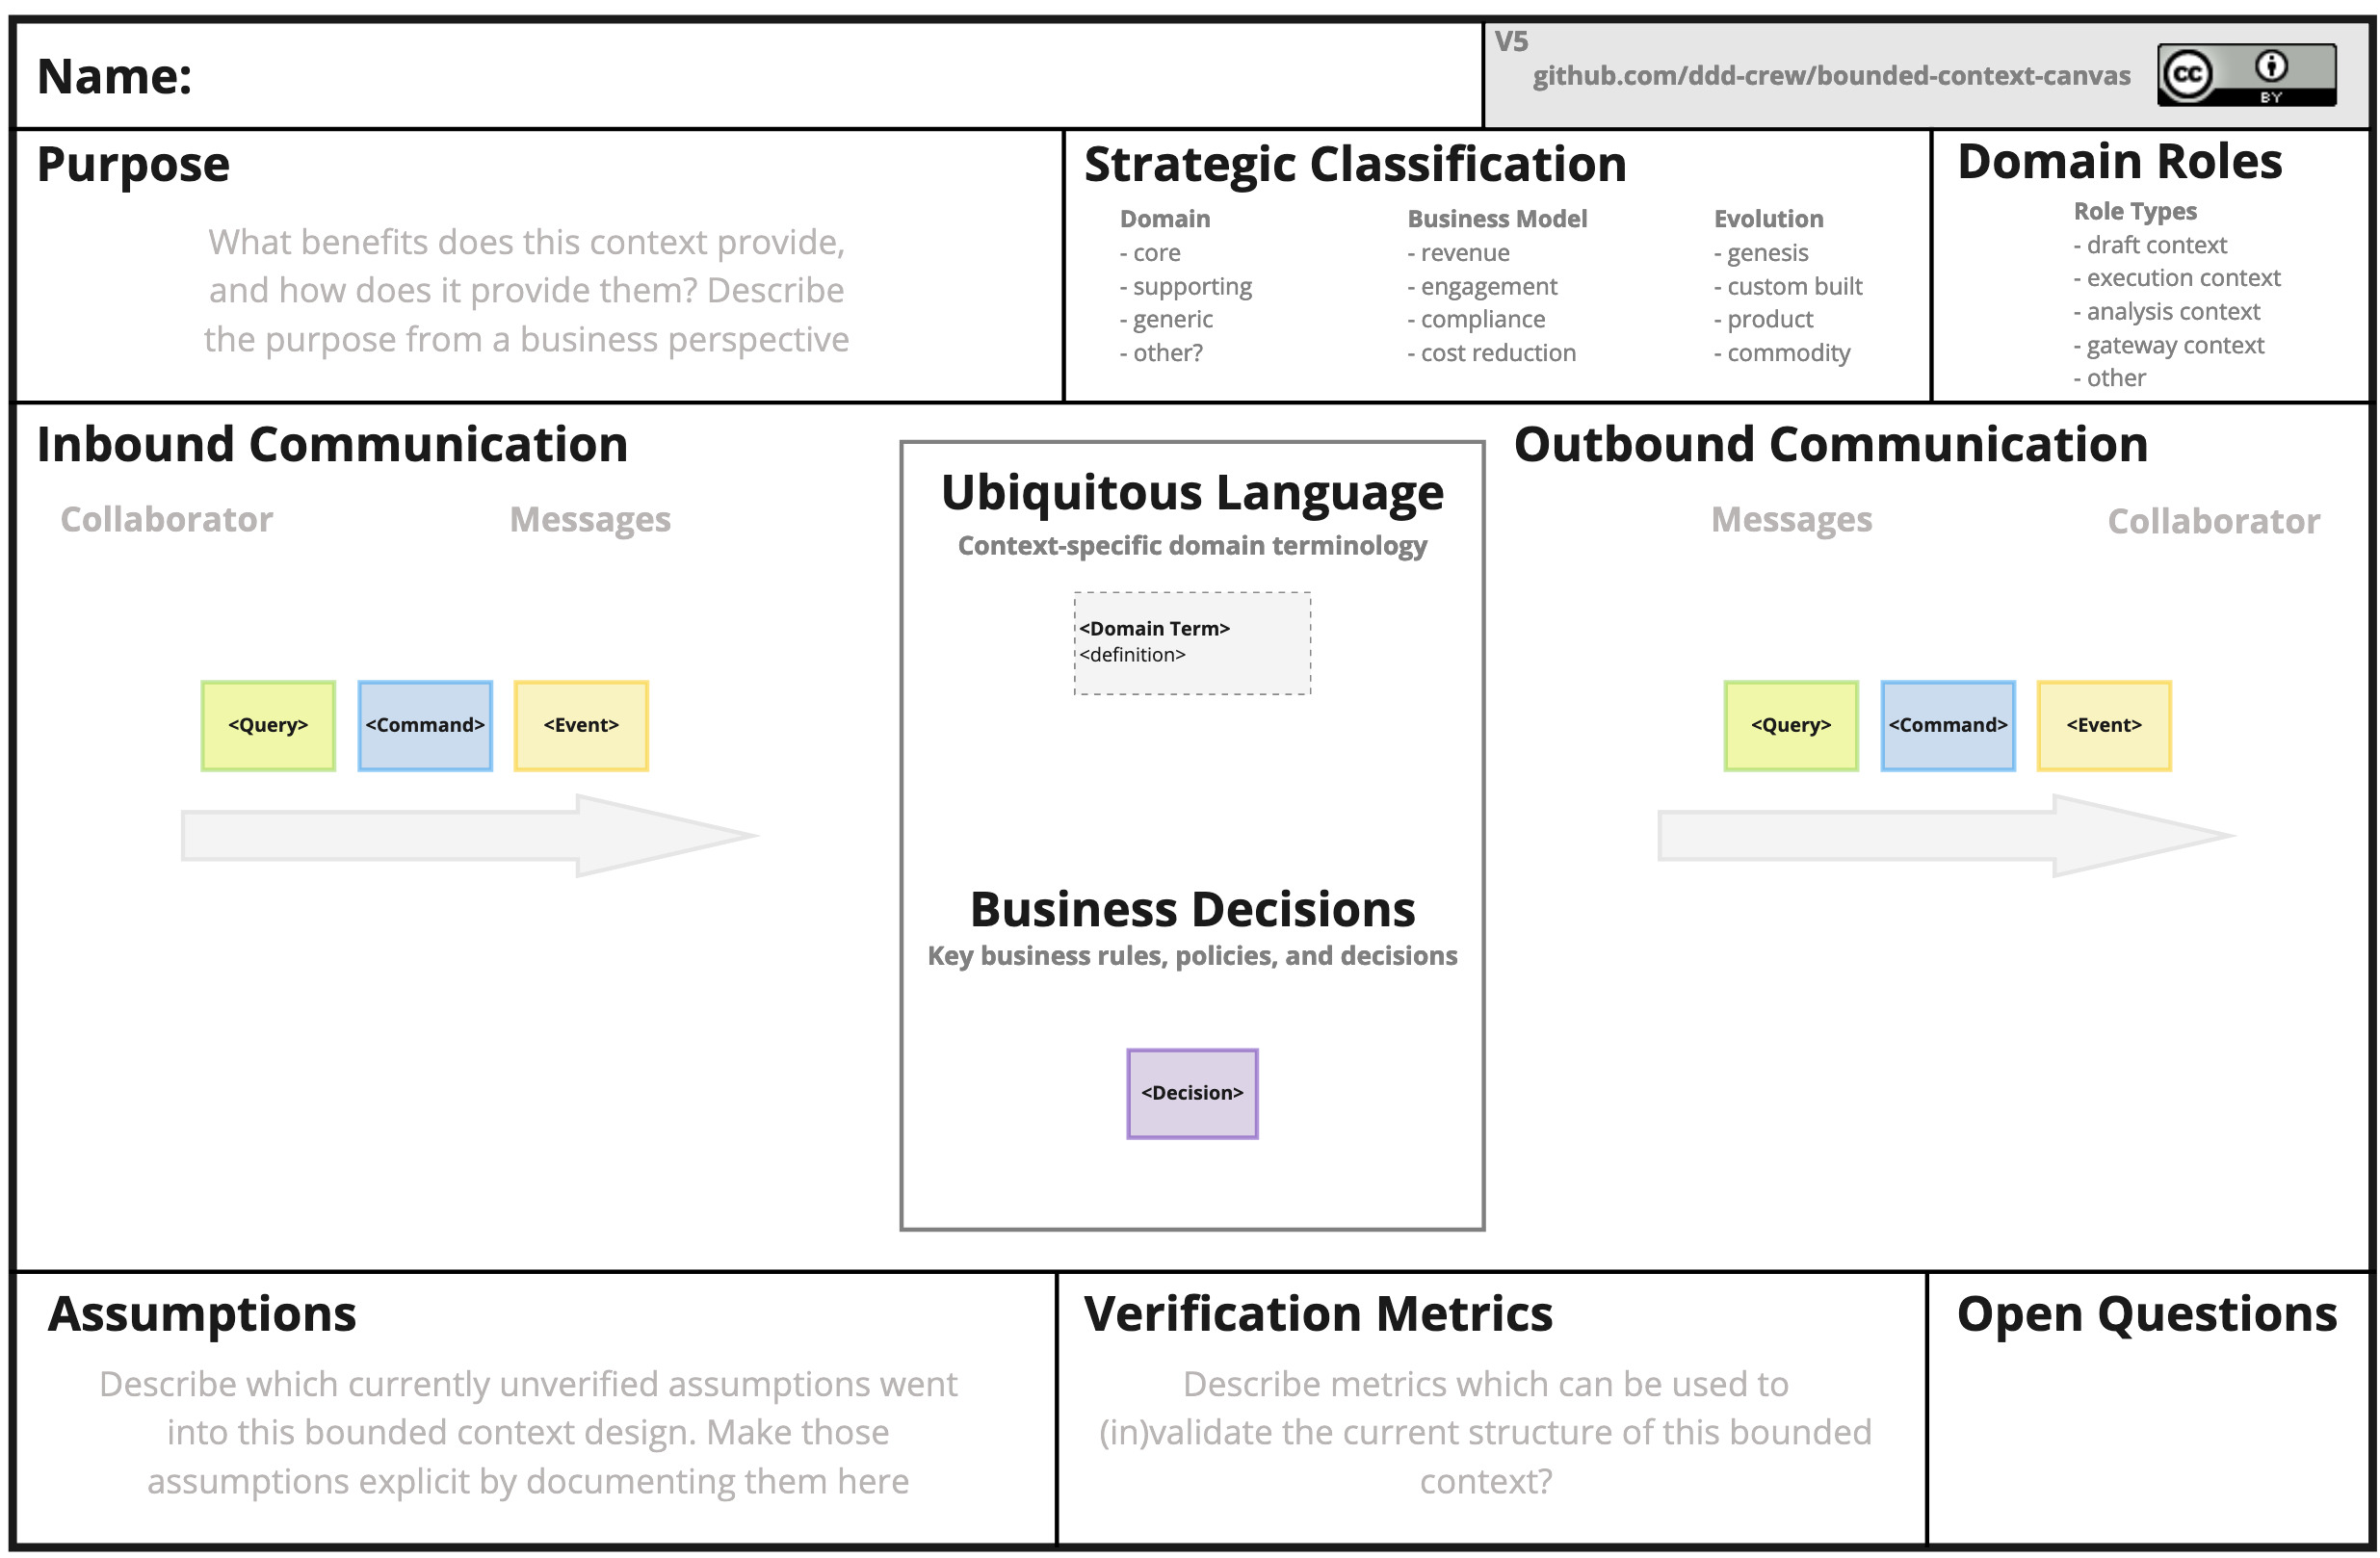
\includegraphics[width=0.8\linewidth]{Images/bounded-context-canvas.jpg}
    \caption{Bounded Context Canvas \href{https://github.com/ddd-crew/bounded-context-canvas}{Bounded Context Canvas Github}}
\end{figure}

\begin{figure}[H]
    \centering
    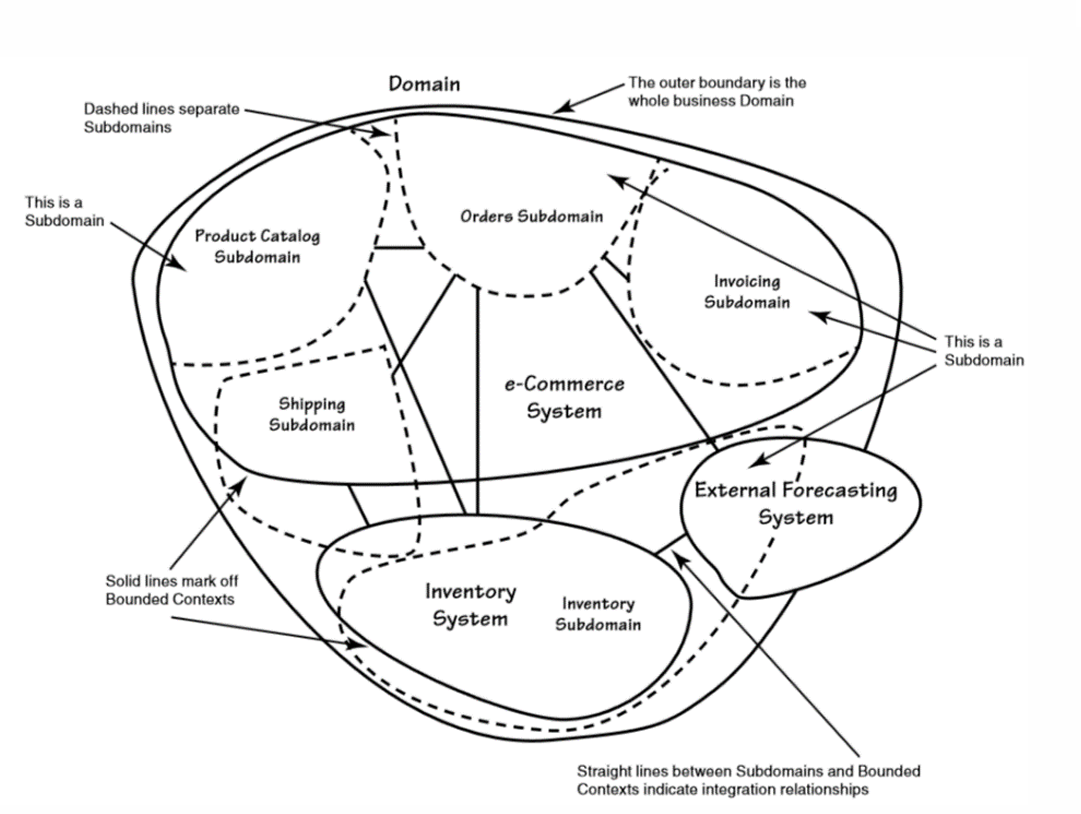
\includegraphics[width=1\linewidth]{Images/subdomains-bounded-context.png}
    \caption{Subdomains vs Bounded Context}
\end{figure}



\begin{figure}[H]
    \centering
    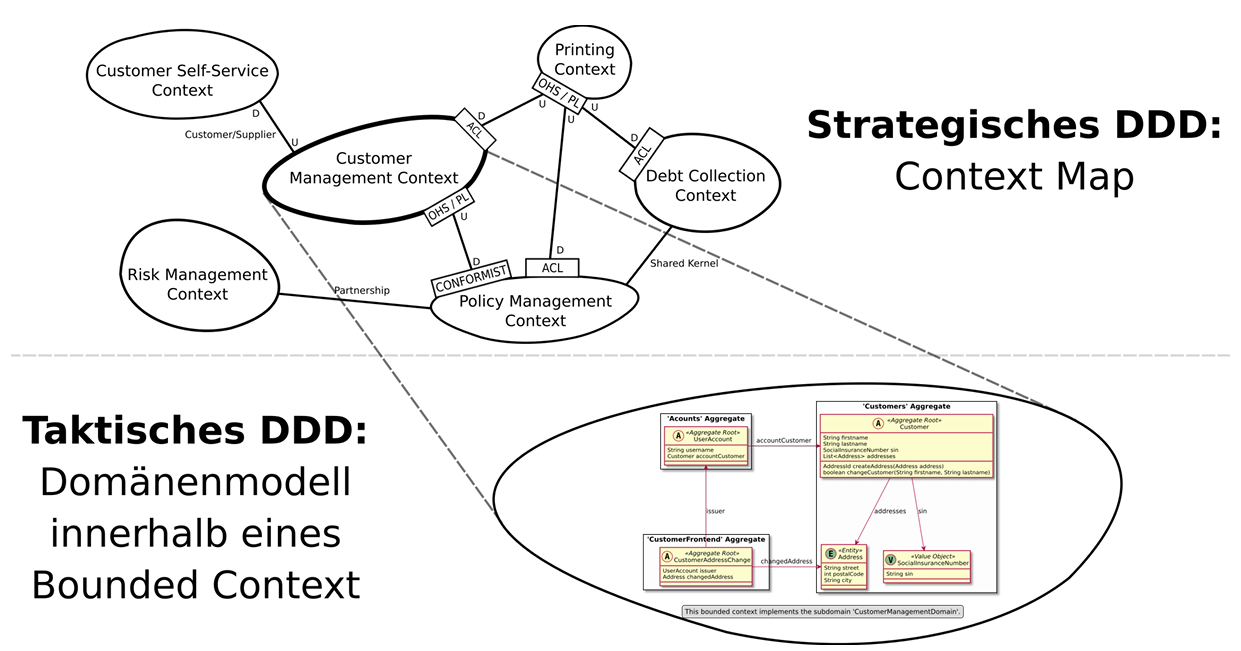
\includegraphics[width=0.75\linewidth]{Images/tactic-strategic.png}
    \caption{Tactic vs Strategic DDD}
\end{figure}

\subsection{BC Context Mapping}
\begin{figure}[H]
    \centering
    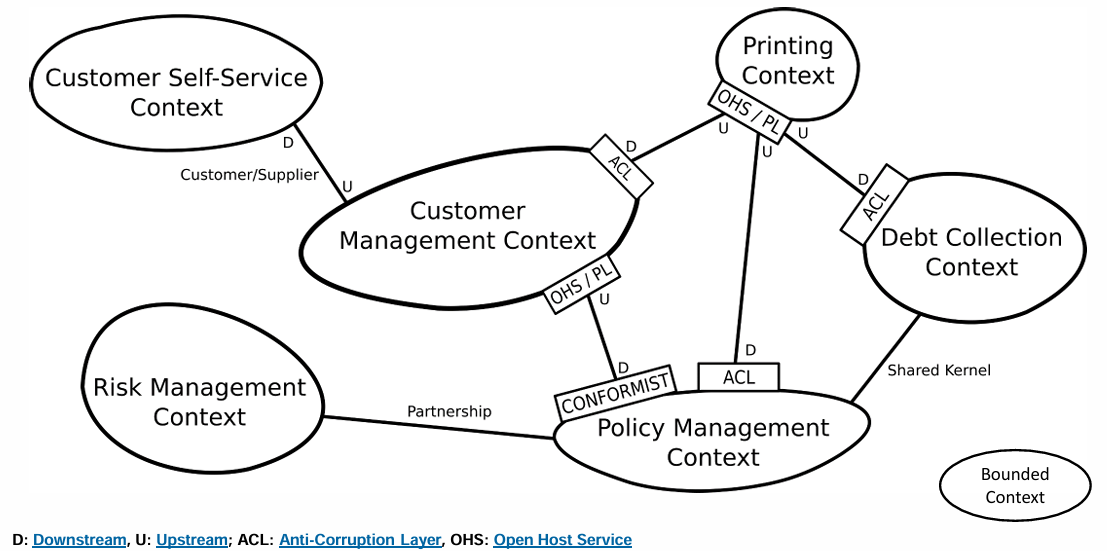
\includegraphics[width=0.75\linewidth]{Images/bc-context-map.png}
    \caption{Strategic DDD Context Map \href{https://contextmapper.org/docs/examples/}{Context Mapper}}
\end{figure}

\begin{description}
    \item[Shared Kernel] Two bounded contexts use a common kernel of code (for example a library) as a common lingua
    franca, but otherwise do their other stuff in their own specific way. This is a symmetric relationship.
    \item[Open Host Service] A Bounded Context specifies a protocol by which any other bounded context can use its services (e.g. 
    a RESTful HTTP service or a SOAP Web service). This protocol may expose a Published Language.
    \item[Published Language] The interacting bounded contexts agree on a common a language (for example a bunch of XML or 
    JSON schemas over an enterprise service bus) by which they can interact with each other.
    \item[Conformist] One BC uses the services of another but is not a stakeholder to that other BC. As such it uses "as-is" 
    (conforms to) the protocols or APIs provided by that bounded context (which may be an OHS).
    \item[Anti-Corruption Layer] One bounded context uses the services of another and is not a stakeholder, but aims to minimize 
    impact from changes in the bounded context it depends on by introducing a set of adapters - an anti
    corruption layer.
    \item[Customer / Supplier] One bounded context uses the services of another and is a stakeholder (customer) of that other 
    bounded context. As such it can influence the services provided by that bounded context. The supplier 
    may expose a PL.
\end{description}
\href{https://www.methodsandtools.com/archive/archive.php?id=97}{Reference}

\begin{figure}[H]
    \centering
    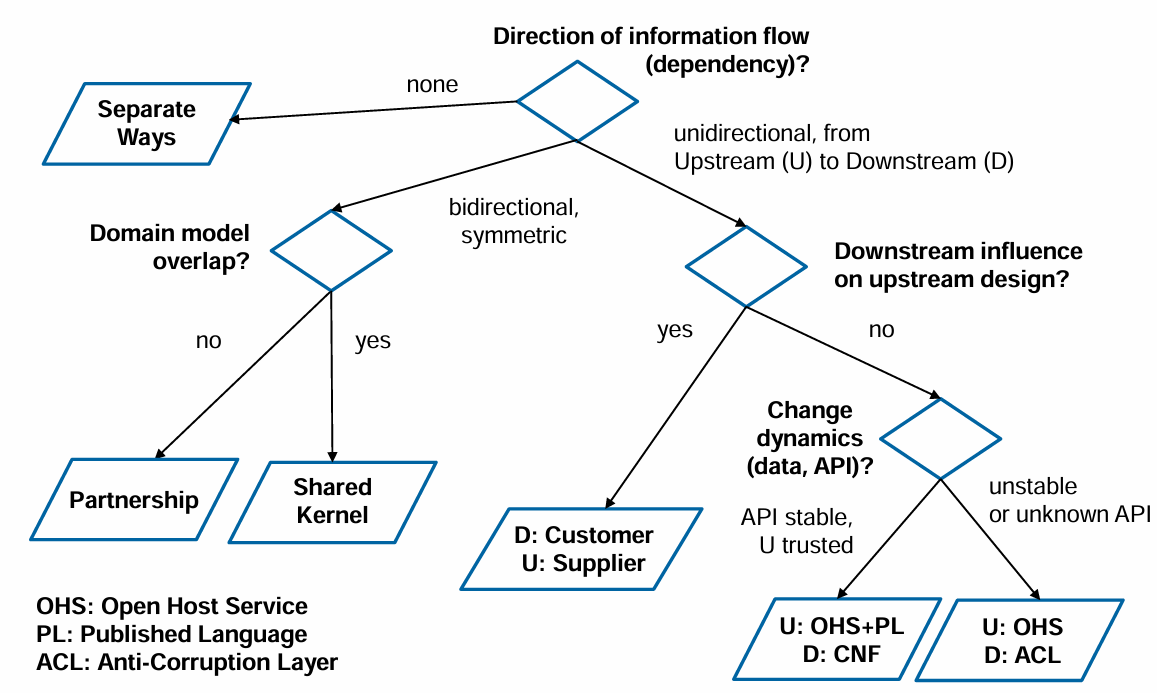
\includegraphics[width=1\linewidth]{Images/context-map-decision-tree.png}
    \caption{Context Map Decision Tree (3+1)}
\end{figure}

\begin{figure}[H]
    \centering
    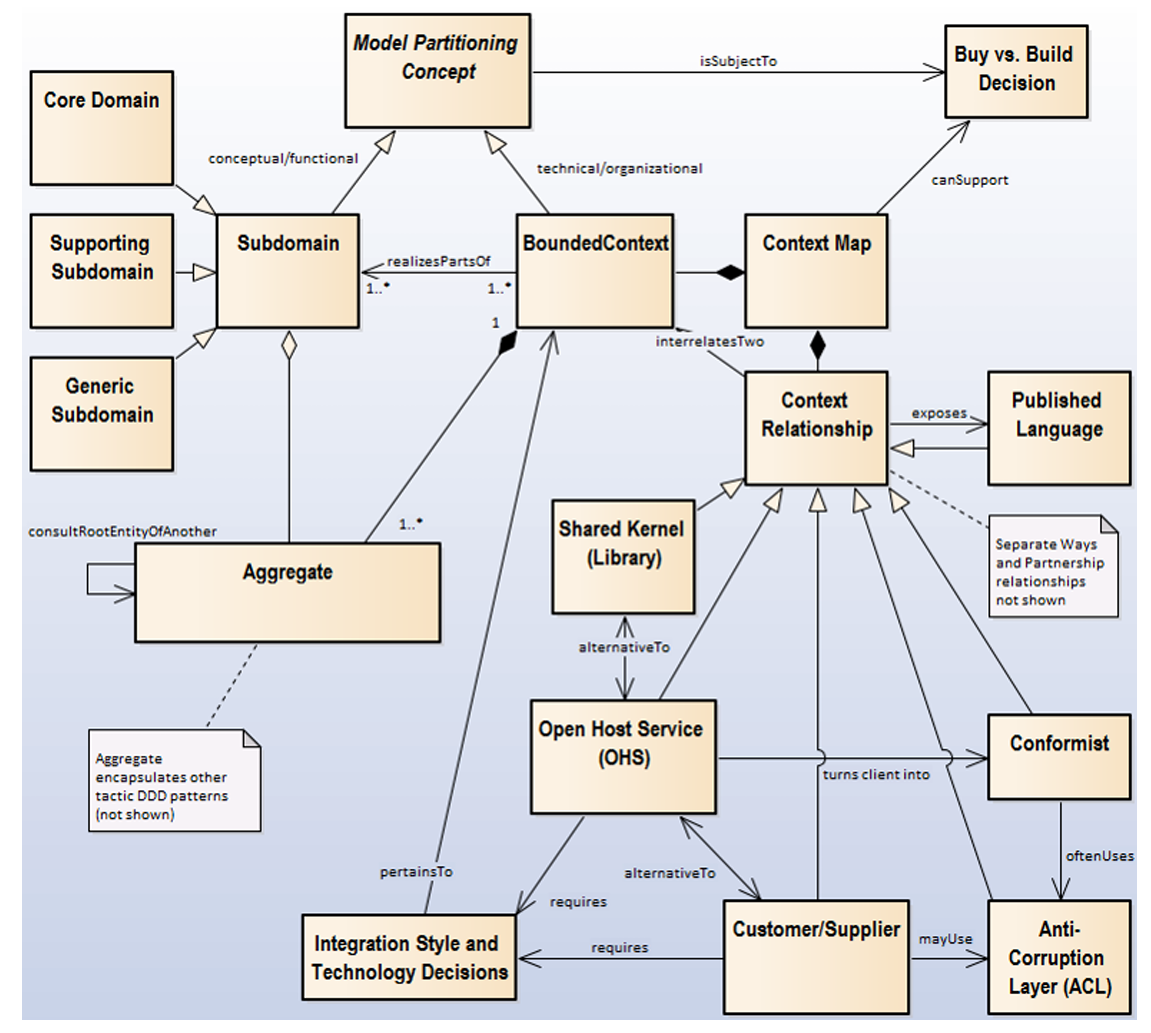
\includegraphics[width=1\linewidth]{Images/strategic-ddd-summary.png}
    \caption{Strategic DDD Patterns and Relationship Summary}
\end{figure}

\newpage
\section{Integration Styles}

In a good integration styles we want to achieve loose coupling while connecting different bounded contexts.
\defn{Loose Coupling Dimensions}{
    Loose coupling has at least four dimensions:
    \begin{description}
        \item[Reference autonomy] Producers and consumers dont know each other. (URI)
        \item[Platform autonomy] Producers and consumers may be located in different technical environments (e.g., 
        containers), can be written in different languages, etc. (HTTP)
        \item[Time autonomy] Producers and consumers access channel at their own pace (Communication is asynchronous,  Data exchanged is persistent). (Messagin)
        \item[Format autonomy] Producers and consumers may use different formats of data exchanged. (EIP)
    \end{description}
}

\subsection{Top Level Remote Communication (Integration Styles)}
\begin{multicols}{2}
    \begin{description}
        \item[File Transfer] Have each application produce files containing information
        that other applications need to consume. Integrators take
        the responsibility of transforming files into different for
       mats. Produce the files at regular intervals according to
        the nature of the business.
        \item[Shared database] Integrate applications by having them store their data in a
        single Shared Database.
        \item[Remote Procedure Calls]  Develop each application as a large-scale object or compo
        nent with encapsulated data. Provide an interface to allow
         other applications to interact with the running application.
        \item[Messaging] Use Messaging to transfer packets of data frequently, im
        mediately, reliably, and asynchronously, using customizable
         formats. Is a known use of the Pipes and Filters pattern.
    \end{description}
    \columnbreak

    Eight fallacies of distributed systems from \href{http://www.drdobbs.com/errant-architectures/184414966}{Fowler}:
    \begin{enumerate}
        \item The network is reliable
        \item Latency is zero
        \item Bandwidth is infinite
        \item The network is secure
        \item Topology does not change
        \item There is one administrator
        \item Transport cost is zero
        \item The network is homogeneous
    \end{enumerate}
\end{multicols}
\defn{Web as Integration Style}{
    You can design web API to be viewable as an asynchronous connector technology.
    With this, resources take the place of messaging queues or channels.
}

\begin{figure}[H]
    \centering
    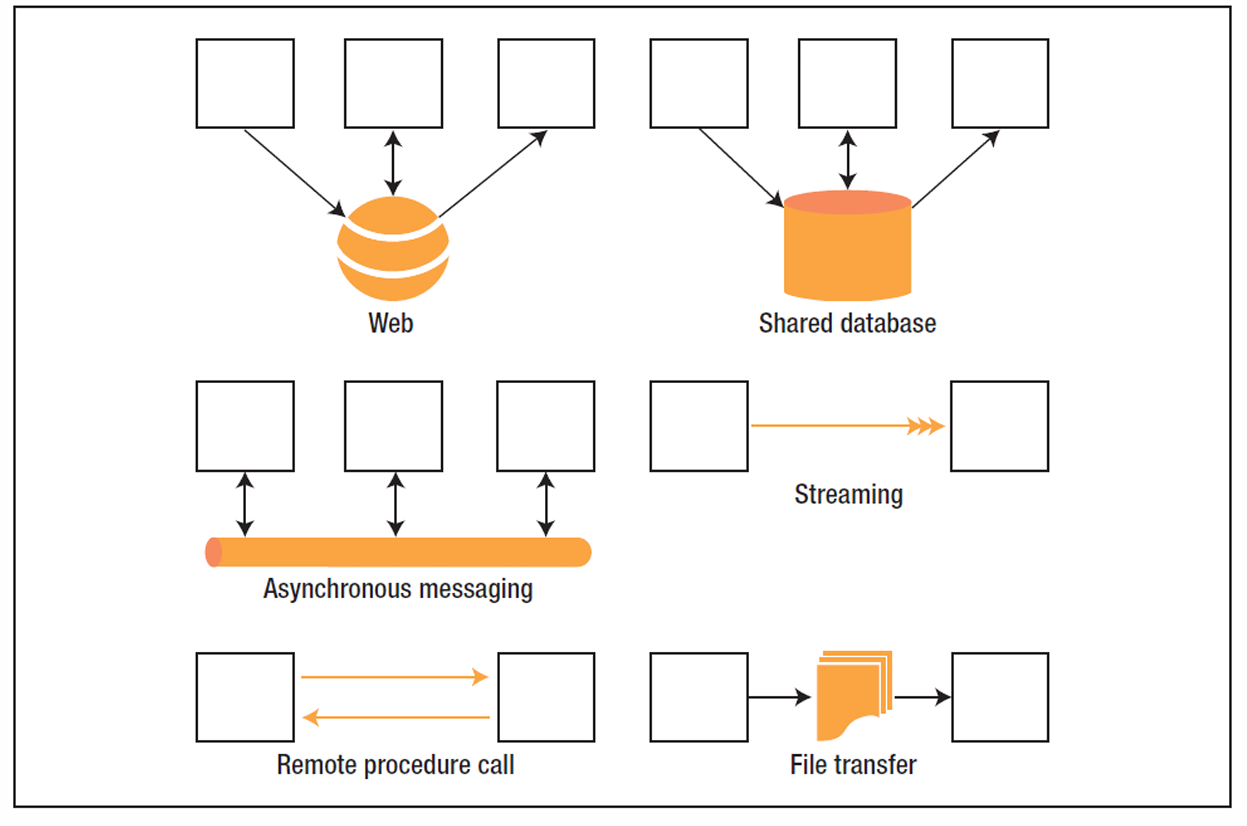
\includegraphics[width=0.75\linewidth]{Images/general-integration-styles.png}
    \caption{Six General Integration Styles}
\end{figure}

\subsection{Messaging System (Middleware)}
Messaging capabilities are typically provided by a separate software system called a messaging system or 
message-oriented middleware (MOM), which is comparable to database systems that manage data 
persistence:
\begin{itemize}
    \item Database administrator populates database with schema for application data; MOM administrator 
    configures the messaging system with channels that define the paths of communication between the 
    applications. Messaging system manages sending and receiving of messages.
    \item Database makes sure each data record is safely persisted, and likewise main task of messaging system 
    is to move messages from the sender's computer to the receiver's computer in a reliable fashion.
\end{itemize}
The reason a messaging system is needed to move messages from one computer to 
another is that computers and the networks that connect them are inherently unreliable:
\begin{itemize}
    \item Just because one application is ready to send a communication does not mean that the 
    other application is ready to receive it.
    Even if both applications are ready, the network may not be working, or may fail to 
    transmit the data properly.
    \item A messaging system overcomes these limitations by repeatedly trying to transmit the 
    message until it succeeds. Under ideal circumstances, the message is transmitted 
    successfully on the first try, but circumstances are often not ideal.
\end{itemize}
To achieve this, an established abstraction is used: 
\defn{Channels}{
    Channels a.k.a. Queues are a fundamental logical concept realized via several physical network connections.
    There are typically multiple middleware instances involved which send, receive and process messages and make them
    available to different endpoints.
}
There are different protocols which implement data communication, one
of these is AMQP which is a peer to peer transport protocol operating over TCP. AMQP supports message headers and properties
which enables the implementation of EIP patterns. ActiveMQ is a popular messaging implementation that supports AMQP.
\\\\
Messaging has the \textbf{advantage} to enable loose coupling in the time, platform and reliability dimensions, but it comes at a price.
For example do middleware design impose a more complex architecture and have thus more design, test and management effots.
But it also comes with several \textbf{disadvantages}:
\begin{description}
    \item[Complexity] Asynchronous messaging requires developers to work with an event-driven programming model. 
    Application logic can no longer be coded in a single method that invokes other methods, but the logic is 
    not split up into a number of event handlers that respond to incoming messages. Such a system is more 
    complex and harder to develop and debug. For example, the equivalent of a simple method call can 
    require a request message and a request channel, a reply message and a reply channel, a correlation 
    identifier and an invalid message queue (as described in Request-Reply)
    \item[Sequencing Issues] Message channels guarantee message delivery, but they do not guarantee when the message will be 
    delivered. This can cause messages that are sent in sequence to get out of sequence. In situations 
    where messages depend on each other special care has to be taken to re-establish the message 
    sequence.
    \item[Synchronous Scenarios] Not all applications can operate in a send-and-forget mode. If a user is looking for airline 
    tickets, he or she is going to want to see the ticket price right away, not after some 
    undetermined time. Therefore, many messaging systems need to bridge the gap between 
    synchronous and asynchronous solutions.
    \item[Performance] Messaging systems do add some overhead to communication. It takes effort to make data 
    into a message and send it, and to receive a message and process it. If you have to 
    transport a huge chunk of data, dividing it into a gazillion small pieces may not be a smart 
    idea. For example, if an integration solution needs to synchronize information between two 
    existing systems, the first step is usually to replicate all relevant information from one 
    system to the other. For such a bulk data replication step as provided by most ETL tools 
    are much more efficient than messaging. Messaging is best suited to keeping the systems 
    in sync after the initial data replication.
    \item[Platform Support]  Many proprietary messaging systems are not available on all platforms. Often times it is easier to FTP a 
    file to another platform than accessing it via a messaging system.
    \item[Vendor Lock-In] Many messaging system implementations rely on proprietary protocols. Even common messaging 
    specifications such as JMS do not control the physical implementation of the solution. As a result, 
    different messaging systems usually do not connect to one another. This can leave you with a whole 
    new integration challenge: integrating multiple integration solutions!
\end{description}

\newpage
\subsection{Enterprise Integration Patterns (EIP) / Messaging}
EIP (Gregor Hohpe 2003) handles the integration of different bounded contexts.
It was originally suggested by Martin Fowler and K. Brown.
EIP provide a conceptual design space for the Messaging style.

\exm{Recapitulate}{
    Let us recapitulate the state of affairs in architectural synthesis after Lessons 3 to 8: 
    candidate components have been identified and specified; some or all of these components have been realized
    (as a consequence of a make/build decision) or procured (following a buy decision). Tactic and strategic DDD patterns might
    (but do not have to) be used along this way (for instance, during component realization with object-oriented pro gramming).
    Next, these components need to be stitched together to yield end-to-end applications that imple mentfunctional requirements
    (expressed as use cases and/or user stories) and satisfy NFRs (including quality attributes): integration is required.
}
\begin{multicols}{2}
    In essence, a message is send in five steps:
    \begin{enumerate}
        \item Create
        \item Send
        \item Deliever
        \item Receive
        \item Process
    \end{enumerate}

    The API Primitives are very simple and consist from basically out of Write, Consume, Non-Consuming Read.
    Even with this easy API there are still many design choices to be made like
    how the message intent (command vs data), response (request-reply), data sequencing, message performance (message expiration),
    QoS (guaranteed delivery, transactionality, idempotency) is to be structured.
\end{multicols}

\begin{figure}[H]
    \centering
    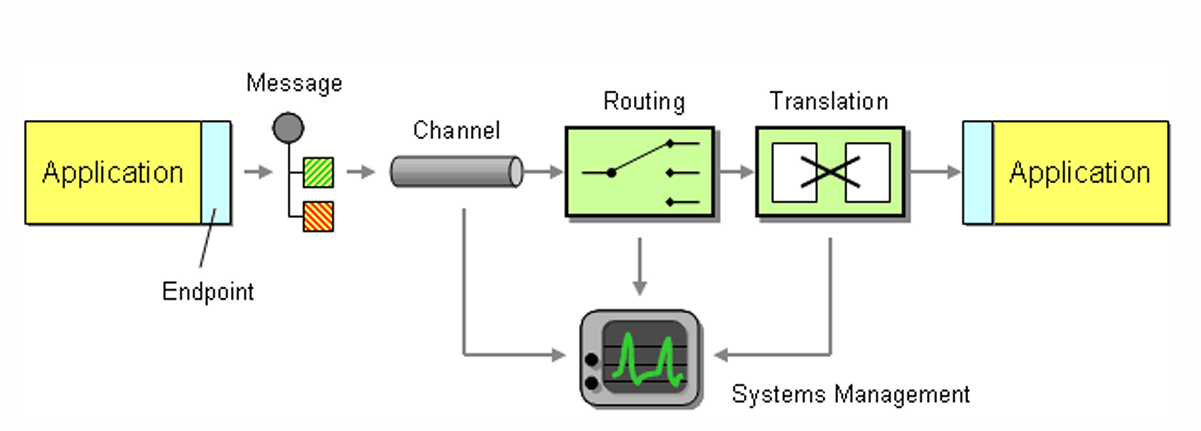
\includegraphics[width=0.75\linewidth]{Images/eip-overview.png}
    \caption{EIP Summary}
\end{figure}
\newpage
\subsection{Jakarta Messaging API (JMS)}
Jakarta Messaging API defines structures for the user. There exists Point-to-Point channels (\textbf{Queue API}) or 
Publish-Subcribe channels (\textbf{Topic API}) out of the box, the API between the object is different where as one uses the 
Queue API and the other the Topic API. The messages itselves can have different types. Typically one would 
use text messages, serializable objects or binary. The JMS API support general QoS settings via headers.

\begin{description}
    \item[Message Enpoint] @JMSTemplate (@Controller)
    \item[Event-Driven Consumer] @JMSListener
    \item[Service Activator] @ServiceActivator (+ XML-Configuration)
    \item[Content-Based Router] @Router (+ XML-Configuration)
    \item[Content Enrichter] @Transformer, @Enricher
\end{description}

\newpage
\subsection{Important EIP}
\href{https://www.enterpriseintegrationpatterns.com/ramblings/eip1_examples_updated.html}{EIP Pattern Reference}
\begin{multicols}{2}
    \begin{itemize}
        \item Document Message Pattern. Use a Document Message to reliably transfer a data structure between applications.
        \item Command Message Pattern. Use a Command Message to reliably invoke a procedure in another application.
        \item \textbf{Point-to-Point Channel*}. Send the message on a Point-to-Point Channel, which ensures that only one receiver will 
        receive a particular message.
        \item \textbf{Publish-Subscribe Channel*}.  Send the event on a Publish-Subscribe Channel, which delivers a copy of a particular event to each receiver.
        \item \textbf{Guaranteed Delivery Pattern*}. Use Guaranteed Delivery to make messages persistent so that they are not lost even if the 
        messaging system crashes.
        \item Message Endpoint Pattern. Connect an application to a messaging channel using a Message Endpoint, a client of the 
        messaging system that the application can then use to send or receive messages.
        \item \textbf{Event-Driven Consumer*}. The application should use an Event-Driven Consumer, one that is automatically handed messages 
        as they're delivered on the channel.
        \item \textbf{Competing Consumers*}. Create multiple Competing Consumers on a single channel so that the 
        consumers can process multiple messages concurrently.
        \item \textbf{Polling Consumers*}. The application should use a Polling Consumer, one that explicitly makes a call when it 
        wants to receive a message.
        \item \textbf{Selective Consumer*}. Make the consumer a Selective Consumer, one that filters the messages delivered by its 
        channel so that it only receives the ones that match its criteria.
        \item Request-Reply Pattern. Send a pair of Request-Reply messages, each on its own channel.
        \item Return Address. The request message should contain a Return Address that indicates where to send the reply message.
        \item Message Expiration.  Set the Message Expiration to specify a time limit how long the message is viable.
        \item Dead Letter Channel Pattern. When a messaging system determines that it cannot or should not deliver a message, it may elect to move 
        the message to a Dead Letter Channel.
        \item \textbf{Transactional Client Pattern*}. Use a Transactional Client to make the clients session with the messaging system 
        transactional so that the client can specify transaction boundaries.
        \item \textbf{Message Routing Pattern*}. Insert a special filter, a Message Router, which consumes a Message from one Message 
        Channel and republishes it to a different Message Channel depending on a set of conditions. 
        \item (...)
    \end{itemize}
\end{multicols}
\newpage

\begin{figure}[H]
    \centering
    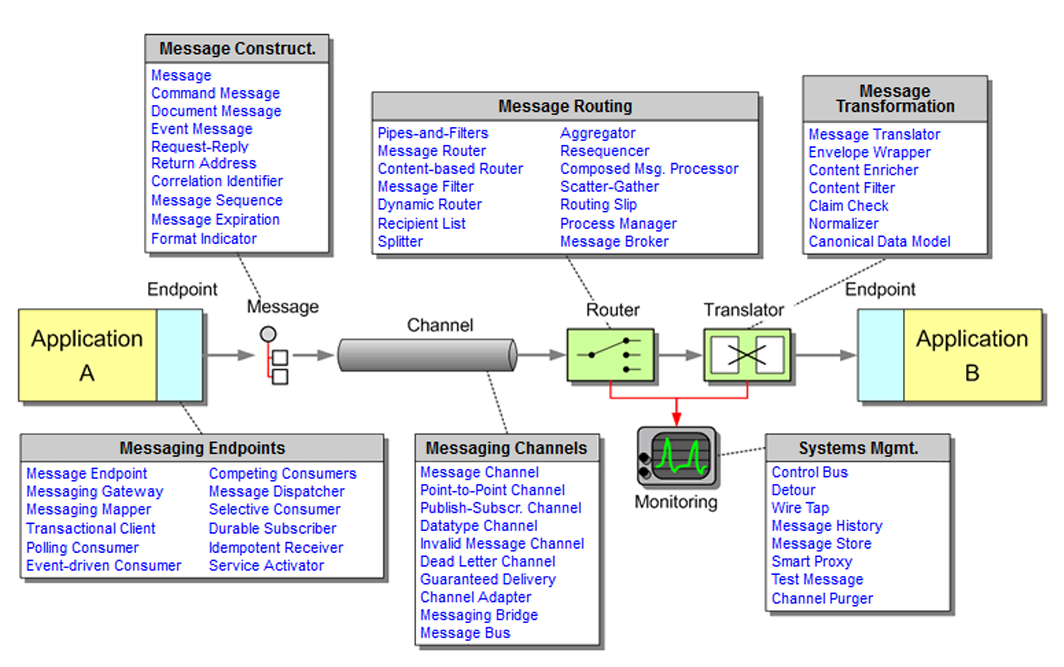
\includegraphics[width=1\linewidth]{Images/eip-categories.png}
    \caption{EIP Categories}
\end{figure}

\begin{figure}[H]
    \centering
    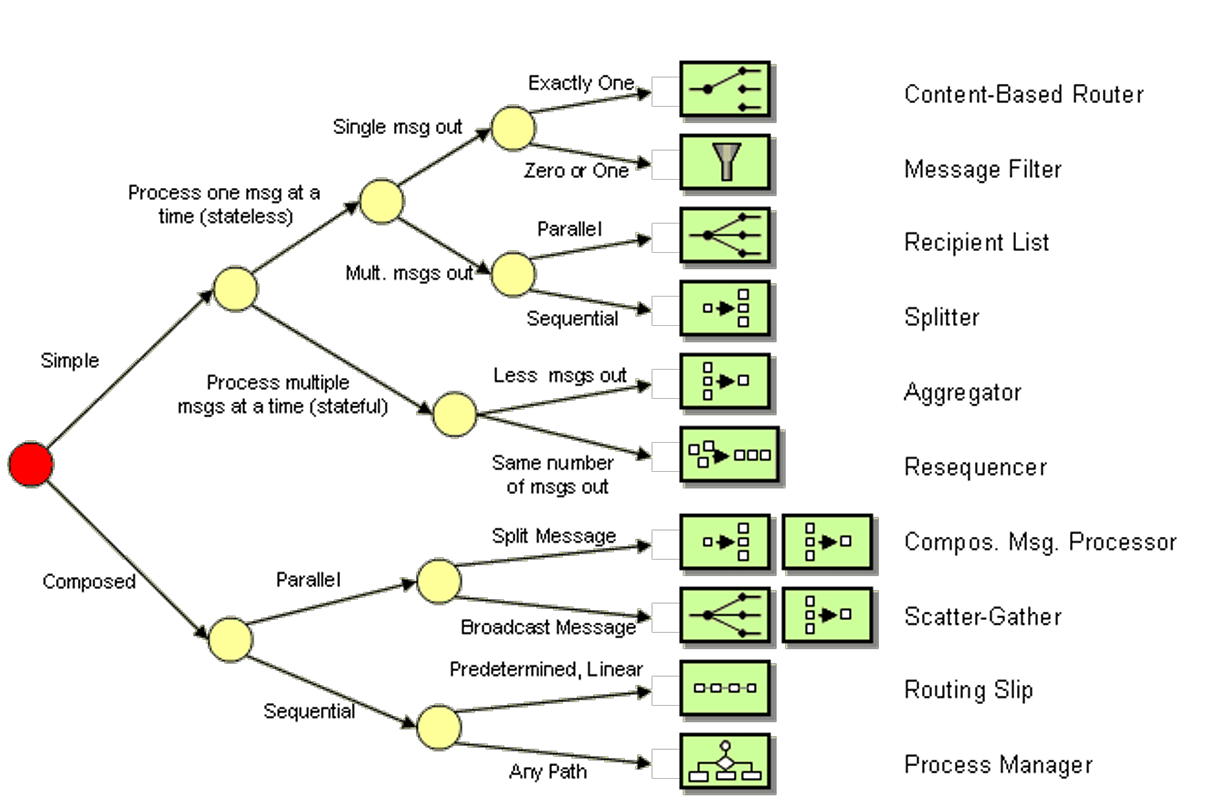
\includegraphics[width=0.9\linewidth]{Images/eip-message-routing-categories.png}
    \caption{EIP Routing}
\end{figure}

\begin{multicols}{2}
    \textbf{Message Routing Patterns:}
    \begin{itemize}
        \item \textbf{Content-Based Router Pattern*}. Use a Content-Based Router to route each message to the correct recipient based on message content. 
        \item \textbf{Recipient List Pattern*}. Define a channel for each recipient. Then use a Recipient List to inspect an incoming message, determine 
        the list of desired recipients, and forward the message to all channels associated with the recipients in the 
        list.
        \item Splitter Pattern. Use a Splitter to break out the composite message into a series of individual messages, each containing 
        data related to one item.
        \item \textbf{Aggregator Pattern*}. Use a stateful filter, an Aggregator, to collect and store individual messages until a complete set of related 
        messages has been received. Then, the Aggregator publishes a single message distilled from the individual 
        messages.
        \item (...)
    \end{itemize}
    \textbf{Message Transformation (Mediation):}
    \begin{itemize}
        \item \textbf{Message Translator Pattern*}. Use a special filter, a Message Translator, between other filters or applications to translate 
        one data format into another.
        \item Content Filter Pattern.  Use a Content Filter to remove unimportant data items from a message leaving only important items.
        \item Content Enricher Pattern. Use a specialized transformer, a Content Enricher (a.k.a. Data Enricher), to access an external data source 
        in order to augment a message with missing information.
        \item (...)
    \end{itemize}
\end{multicols}

\newpage
\section{Coupling - Tradeoff Analysis}
\begin{figure}[H]
    \centering
    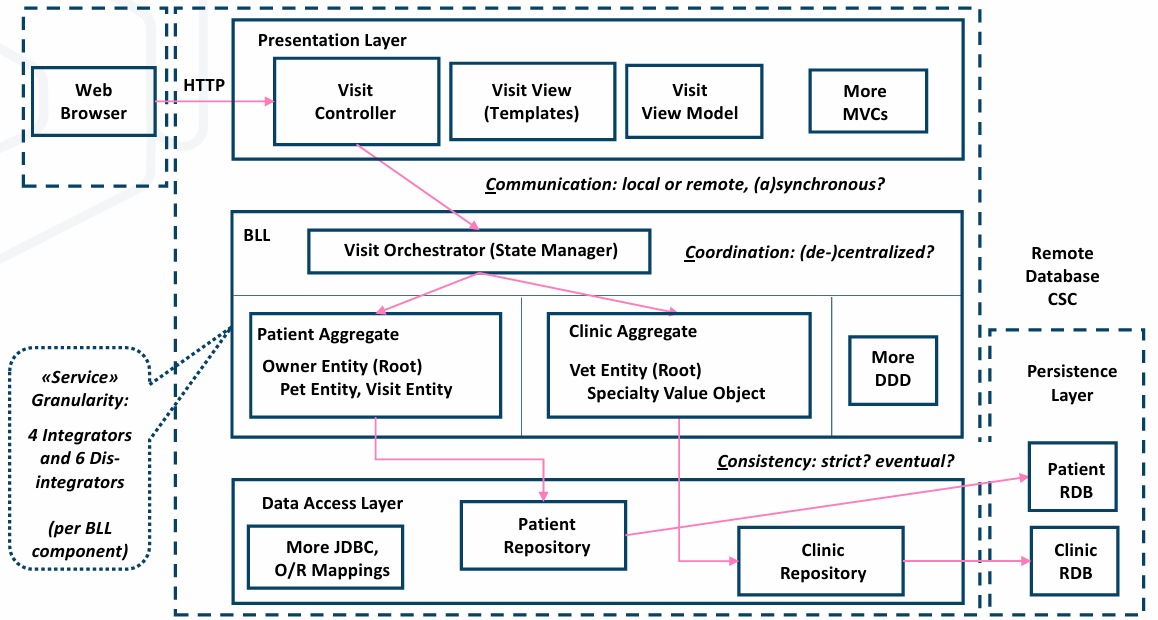
\includegraphics[width=1\linewidth]{Images/coupling-tradeoff.png}
    \caption{Tradeoffs in Coupling}
\end{figure}

\begin{enumerate}
    \item Find what parts are coupled together
    \item Analyze how they are coupled to one another
    \item Assess tradeoffs by determine the impact of change to interdependent systems
\end{enumerate}

\begin{figure}[H]
    \centering
    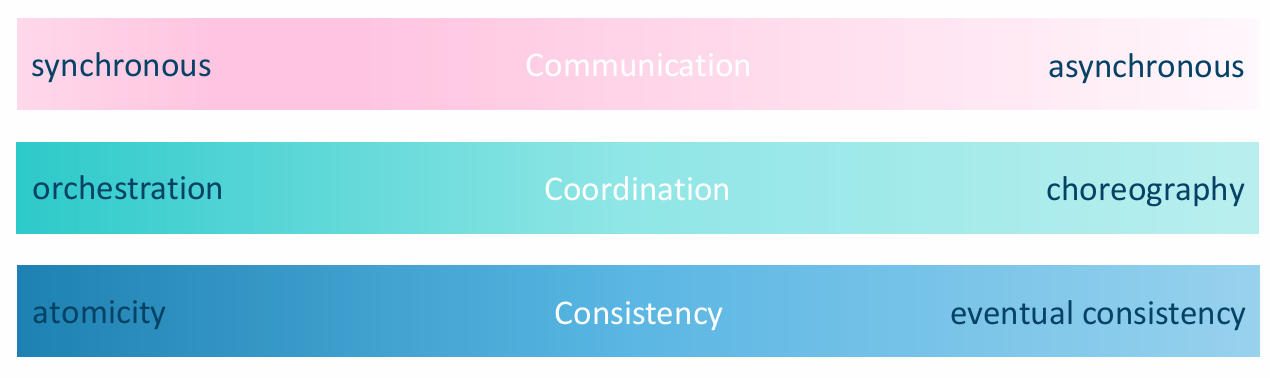
\includegraphics[width=1\linewidth]{Images/coupling-elements.png}
    \caption{Coupling Tradeoff Elements}
\end{figure}
\newpage
\subsection{Communication}
\subsubsection{Synchronous}

\begin{multicols}{2}
    \textbf{Contra}:
    \begin{itemize}
        \item Performance impact on highly interactive systems
        \item Creates dynamic entanglements
        \item Creates limitaions in distributed architecture
    \end{itemize}
    \columnbreak
    \textbf{Pro}:
    \begin{itemize}
        \item Easy to model transactional behaviour
        \item Mimics non-distributed method calls
        \item Easier to implement
    \end{itemize}
\end{multicols}
\subsubsection{Asynchronous}
\begin{multicols}{2}
    \textbf{Contra}:
    \begin{itemize}
        \item Complex to build and debug
        \item Presents difficulties for transactional behaviors
        \item Error handling needs to cover more cases
    \end{itemize}
    \textbf{Pro}:
    \begin{itemize}
        \item Allows highly decoupled systems
        \item Common performance tuning techniques
        \item High performance and scale
    \end{itemize}
\end{multicols}
\newpage

\begin{figure}[H]
    \centering
    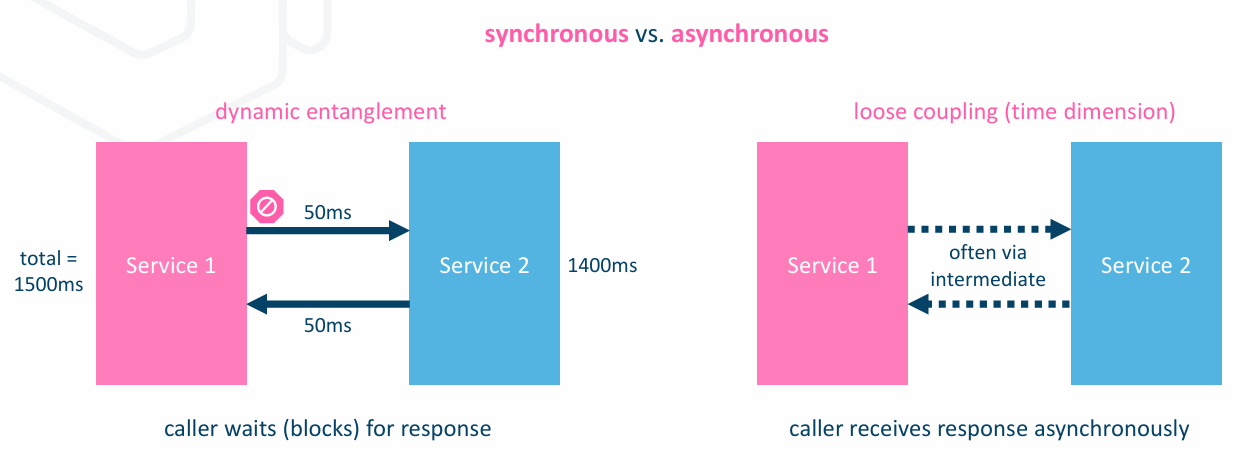
\includegraphics[width=1\linewidth]{Images/coupling-comm.png}
    \caption{Coupling in Communication}
\end{figure}

\subsection{Coordination}
\begin{figure}[H]
    \centering
    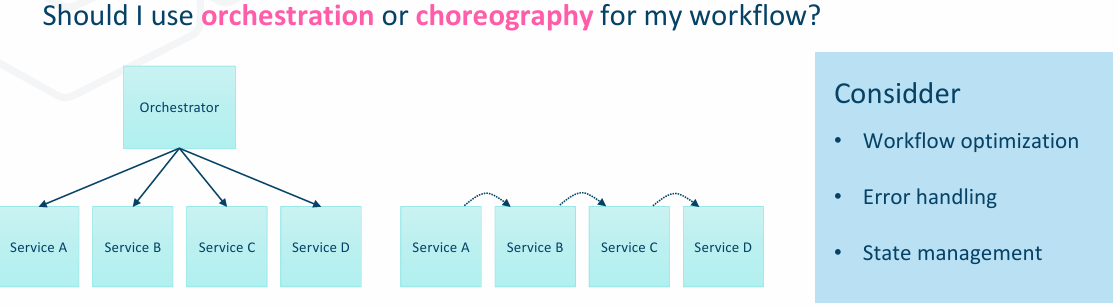
\includegraphics[width=1\linewidth]{Images/coupling-coord.png}
    \caption{Coupling in Coordination}
\end{figure}

\begin{figure}[H]
    \centering
    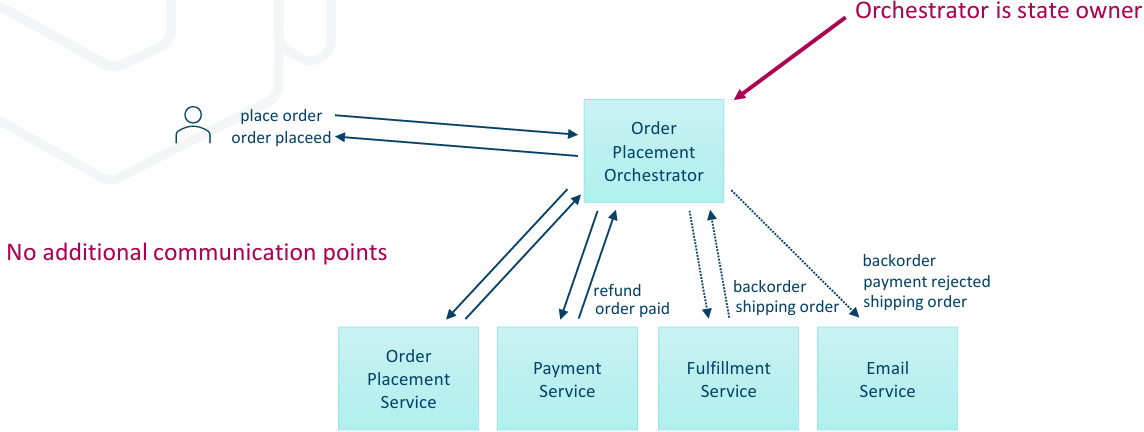
\includegraphics[width=1\linewidth]{Images/workflow-orchestration.png}
    \caption{Workflow Orchestration}
\end{figure}

\newpage
\subsubsection{Orchestration}
\begin{multicols}{2}
    \textbf{Contra}:
    \begin{itemize}
        \item Responsiveness: Orchestrator becomes bottleneck
        \item Fault-Tolerance: Orchestrator becomes SPOF
        \item Scalability: Orchestrator is hard to scale out
        \item Service Coupling: Orchestrator needs to know all services
    \end{itemize}
    \columnbreak
    \textbf{Pro}:
    \begin{itemize}
        \item Centralized Workflow: Good for observability and auditability
        \item Error Handling: Orchestrator handles error states
        \item Recoverability: Orchestrator can take snapshots and attempt to reapply steps
        \item State Management: Orchestrator as single point of truth
    \end{itemize}
\end{multicols}

\subsubsection{Choreography}
\begin{multicols}{2}
    \textbf{Contra}:
    \begin{itemize}
        \item Distributed workflow: Is hard to test, monitor and extend
        \item State Management: Highly distributed by default, The introduction of a state owner mixes choreography with orchestration
        \item Error Handling: Must be implemented in many places
        \item Recoverability: State must be recovered in each service
    \end{itemize}
    \columnbreak
    \textbf{Pro}:
    \begin{itemize}
        \item Responsiveness: No central service that might become a bottleneck
        \item Fault tolerance: No SPOF
        \item Scalability: Each service can be scaled up and down independently
        \item Service decoupling: Each service only works with its direct neighbours
    \end{itemize}
\end{multicols}

\begin{figure}[H]
    \centering
    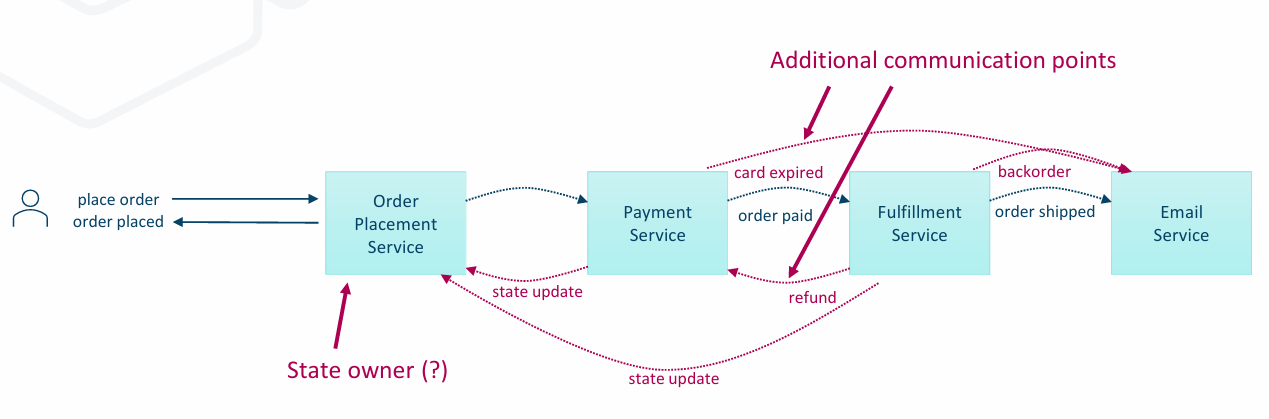
\includegraphics[width=1\linewidth]{Images/workflow-choreography.png}
    \caption{Workflow using Choreography}
\end{figure}
\newpage

\newpage
\subsection{Consistency}
This describes wether the workflow communication requires atomicity or can fully utilize eventuel consistency.
Atomicity garantees that each transaction is treated as a single unit, which either suceeds or fails completely.
Eventuel consistency informally guarantees that, if no new updates are made to a given data item, eventually all accesses to that item will return the last updated value.
This is not the same as in german with "eventuell", but it rather translates to "schlussendlich".

\subsection{Service Granularity}
\begin{multicols}{2}
    \textbf{Disintegrator} provide guidance and justification for when to break a service into smaller pieces.
    \begin{description}
        \item[Service Scope and Function] Is the service doing too many unrelated things?
        \item[Code Volatility] Are changes isolated to only one part of the service?
        \item[Scalability and Troughput] Do parts of the service need to scale differently?
        \item[Fault Tolerance] Are there errors that cause critical functions to fail within the service?
        \item[Security] Do some parts of the service need higher security levels than others?
        \item[Extensibility] Is the service always expanding to add new contexts?   
    \end{description}
    \columnbreak
    \textbf{Integrators} provide guidance and justification for putting services back  toghether or not breaking apart a service in the first place.
    \begin{description}
        \item[Database Transactions] Is an ACID transaction required between separate services?
        \item[Workflow and Choreography] Do services need to talk to one another?
        \item[Shared Code] Do services need to share code among one another?
        \item[Database Relationships] Although a service can be broeken apart, can the data it uses be broken apart as well?    
    \end{description}
\end{multicols}
\newpage

\section{Service Orientation}
\defn{Service}{
    A service is similar to a component in that it's used by foreign applications. The main 
    difference is that I expect a component to be used locally (think jar file, assembly, DLL, or a 
    source import). A service will be used remotely through some remote interface, either 
    synchronous or asynchronous (e.g. Web service, messaging system, RPC, or socket.)
    \href{http://martinfowler.com/articles/injection.html}{Martin Fowler}
}

\subsection{Patterns used for Defining SOA from PoEAA}
\begin{figure}[H]
    \centering
    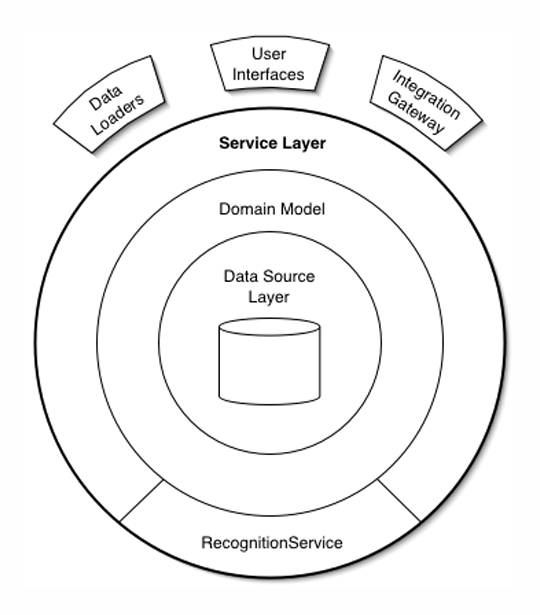
\includegraphics[width=0.35\linewidth]{Images/service-layer-pattern.png}
    \caption{Service Layer Pattern (PoEAA)}
\end{figure}

With the Service Layer Pattern we want to hide complex domain models from the presentation layer.
For this we define an applications boundary with a layer of services that establish a set of available operations
and coordinates the applications response in each operation.

Some other responsibilities could include: Role-Based Access Control (RBAC), transaction control, business-level undo (compensation),
activity logging, metering, monitoring and exception handling.
\newpage


\begin{figure}[H]
    \centering
    \includegraphics[width=0.6\linewidth]{Images/remote-facade.png}
    \caption{Remote Facade Pattern (PoEAA)}
\end{figure}

\begin{figure}[H]
    \centering
    \includegraphics[width=0.75\linewidth]{Images/data-transfer-object.png}
    \caption{Data Transfer Option Pattern (PoEAA)}
\end{figure}
\newpage

\subsection{Service Oriented Architecture (SOA)}
SOA has multiple definitions depending who is answering this question.
\begin{itemize}
    \item A set of services and operations that a business wants to expose to their customers and partners. (Business Domain Analyst)
    \item An architectural style which requires a service provider, a service 
    requestor (consumer) and a service contract (a.k.a. client/server).
    \item A set of architectural patterns such as service layer(with remote 
    facades, data transfer objects), enterprise service bus, service 
    composition (choreography/orchestration), and service registry, 
    promoting principles such as modularity, layering, and loose 
    coupling to achieve design goals such as reuse, and flexibility. (IT-Architect)
    \item A programming and deployment model realized by standards, 
    tools and technologies such as Web services (WSDL/SOAP), 
    RESTful HTTP, or asynchronous message queuing (AMQP etc.) (Developer, Administrator)
    \href{ibm.com}{IBM SOA Solution Stack}
\end{itemize}

\defn{SOA}{
    SOA (and microservices) combine PoEAA, EIP and DDD patterns (and others) in enterprise 
    computing context.
    Service contract must specify syntax, semantics, QoS (interoperability)
}

\begin{figure}[H]
    \centering
    \includegraphics[width=0.75\linewidth]{Images/ibm-microservices.png}
    \caption{From Monolith and Components to SOA and (Micro-)Services}
\end{figure}

Many Enterprise Integration Patterns (EIP) are usable in SOA or in Microservice Design.
E.g some patterns that can be applied:
\begin{description}
    \item[Messaging Gateway] Interoperability between Messaging Systems
    \item[Message Bus] See EIP
    \item[Service Activator] Kind of a middleware see in EIP
    \item[Process Manager] Pattern from Message Routing. Communication of queues are coordinated over the manager (orchestrator)
    There are many available applications for this (EAI, Message Broker)
\end{description}

\begin{figure}[H]
    \centering
    \includegraphics[width=1\linewidth]{Images/napkin-soa.png}
    \caption{Napkin Sketch of SOA Relizations}
\end{figure}

\subsection{Microservices}
Microservices architectures evolved from previous incarnations of Service-Oriented 
Architectures (SOAs) to promote agility and elasticity.
\defn{Microservices Architecture by Fowler}{
    The microservice architectural style is an \textbf{approach to developing a single application 
    as a suite of small services}, each running in its \textbf{own process} and communicating with 
    \textbf{lightweight mechanisms}, often an \textbf{HTTP resource API}.
    Microservices implement SOA, the seven tenets (Newman) including IDEAL (ZIO).
}

\defn{IDEAL Properties (ZIO)}{
    \begin{itemize}
        \item Isolated State
        \item Distribution
        \item Elasticity
        \item Automated Management
        \item Loose Coupling
    \end{itemize}
    \href{https://medium.com/olzzio/what-is-a-cloud-native-application-anyway-part-1-8241e9c71a62}{ZIO Ideal}
}

These services are built around business capabilities and independently deployable by fully automated deployment machinery.
There is a bare minimum of centralized management of these services, which may be written in
different programming languages and use different data storage technologies.
\\\\
They are often deployed in lightweight containers 
and encapsulate their own state, while communicating via message-based remote APIs
 (HTTP, queueing), idealy in a loosely coupled fashion.
They facilitate polyglot programming and persistence, leveraging DevOps practices including decentralized continuous delivery and end-to
end monitoring (for business agility and domain observability).

\defn{Principles (Tenets) of Microservices (Newman)}{
    \begin{itemize}
        \item Model around business concepts (Bounded Context from DDD)
        \item Adopt a culture of automation
        \item Hide internal implementation details
        \item Decentralize all the things
        \item Create independently deployable units
        \item Isolate Failure
        \item Make it highly observable using semantic monitoring with aggregation
    \end{itemize}
}

A microservice can not be sized on only the measured lines of codes.
It dimensions shall be chosen such that it can be developed by a single team, yet be
fully understood by each developer on the theam while beeing able to be replaced by a new implementation if necessary.
On the other hand it must not be to small because this would entail communication and deployment overhead.
Furthermore transactions would span multiple microservices and are hard to manage, the same is true for data consistency.

In a microservice belongs all the data it need to operate while still beeing loosely coupled with others.
New or changed business requirements should ideally lead to changes in just a single microservice including the user interface.

\begin{multicols}{2}
    Some of the \textbf{advantages} can be the following:
    \begin{itemize}
        \item High Velocity due to reduced communication
        \item Some technological independence (e.g. frameworks and languages)
        \item Improved maintainability (in theory)
        \begin{enumerate}
            \item Can be replaced easily
            \item Architecture might be less prone to erosion, because boundaries are harder to overcome
        \end{enumerate}
        \item Suited for cloud deployment due to distributed nature, isolated state and other cloud properties.
        \item Scalability (individually)
        \item Failure safety (due to individual services)
    \end{itemize}
    \columnbreak
    But SOA should not be used blindly, since it also comes with \textbf{disadvantages}:
    \begin{itemize}
        \item Increases complexity e.g. due to more components or coordination
        \item Overhead in communication
        \item More platform requirements
        \item More (...)
    \end{itemize}
\end{multicols}

\subsection{Service Contracts}
A Service contract refers to the definition of a service provided by an application component, detailing its inputs,
outputs and behavior. A service contract is a fundamental building block of service-oriented architecture (SOA) and
serves as a shared understanding between the provider and consumer of the service.
\textbf{Examples of Service Contract Notations are:} OpenAPI Specification, Protocol Buffers (in gRPC context), Web
Service Description Language WSDL, XML Schema Definition XSD.
\begin{itemize}
    \item \href{https://microservice-api-patterns.org/patterns/foundation/APIDescription.html}{API Description pattern}
    in "Patterns for API Design" (a.k.a. MAP)
    \item Open API Specification (f.k.a. Swagger) for technical contract (HTTP-specific);
    Formerly known as Swagger, is an Interface Description Language (IDL) used
    to describe RESTful APIs. It uses a simple YAML or JSON file to describe the structure of an API including its
    endpoints, input and output parameters, authentication methods and other information.
    \item \href{https://microservice-api-patterns.github.io/MDSL-Specification/}{MDSL}
    for technical contract (platform-independent, research prototype);
    Microservice Domain-Specific Language (MDSL) is a language specifically de
    signed to describe the structure and behavior of microservices. It is used to define
    the interface, dependencies, and other aspects of a microservice, and can be used
    to generate code, documentation, and other artifacts.
    \item WSDL: XML Language for Service Descriptions;
    An XML-based language used
    to describe the functionality offered by a web service. It defines the operations
    (methods) that can be called on the service, the inputs and outputs for those
    operations, and the location of the service (the endpoint). It is commonly used in
    context with SOAP interfaces.
    \item SOAP: XML Documents as Service Invocation Messages
\end{itemize}
\section{Patterns for API Design (MAP)}
Microservice API Patterns refer to a set of best practices and design patterns for building and exposing APIs in a
 microservice architecture. MAP helps ensure that APIs are consistent, scalable, secure, and easily consumable by
clients. MAP focuses on message representations. The payload exchanged when APIs are called. (ZIO)
\href{https://api-patterns.org/quickstart-resources}{ZIO Map Reference}

\begin{figure}[H]
    \centering
    \includegraphics[width=0.6\linewidth]{Images/map-categories.png}
    \caption{MAP Categories}
\end{figure}

\subsection{Patterns to know}
\subsubsection{Embedded Entity:}
\begin{description}
    \item[Goal] Avoid exchanging multiple messages when receivers require insights from multiple related information elements.
    \item[Forces] Performance, Scalability, flexibility and modifiability, data quality, freshness, consistency
    \item[Solution] For any relationship that the client has to follow, embed a Data Element in the message that contains
    the data of the target entity (instead of linking to the target entity).
\end{description}

\subsubsection{Pagination:}
\begin{description}
    \item[Goal] Optimize a response to an API client that should deliver large amounts of data with the same structure.
    \item[Forces] Data set size and data access profile, especially number of data records required to be available,
    Variability of data (structure, rate of change),
    Memory availability for a single request (on provider and consumer side),
    Network capabilities (server topology, intermediaries),
    Security and robustness (reliability) concerns
    \item[Solution] \begin{itemize}
        \item  Divide large response data sets into manageable and easy-to-transmit chunks.
        \item Send only partial results in the first response message and inform the consumer how 
        additional results can be obtained/retrieved incrementally. 
        \item Process some or all partial responses on the consumer side iteratively as needed; agree 
        on a request correlation and intermediate/partial results termination policy on consumer 
        and provider side.
    \end{itemize}
    \item[Variants] Cursor-based vs. offset-based
    \item[Consequences] State Management required
\end{description}

\subsubsection{Wish List Pattern:}
\begin{description}
    \item[Goal] Let the API provider know at runtime, what data the client is interested in.
    \item[Forces] Client diversity, message size vs. number of messages, endpoint complexity and more
    \item[Solution] As an API client, provide a WISH LIST in the request that enumerates all desired data elements of the requested resource.
\end{description}

\section{Application State}
Statelessness (of interactions) is emphasized both in SOA and REST.
In this context the state between service consumer/requestor and service provider is focused.
Application and middleware (e.g., queue manager, Web server) are always coupled via invocation API (which can be a local or a remote one).

\defn{Session State Management - Thin Client Options (PoEAA)}{
    \begin{description}
        \item[Client Session State (Rest 3)] HTML/HTTP: cookie, hidden field, URL rewrite (REST: no cookies!); JWT.
        Scales well, but possibly has performance problems and must be secured.
        \item[Server Session State] Uses main memory or proprietary data stores in an application server (e.g., Spring or 
        HTTP session API in JEE servlet container). Persistent HTTP sessions no longer recommended when deploying to a cloud due to 
        scalability and reliability concerns.
        \item[Database Session State] Is well supported in many clouds, e.g. via highly scalable key-value storage (a type of 
        NoSQL database) such as Redis.
    \end{description}
}

\begin{figure}[H]
    \centering
    \includegraphics[width=1\linewidth]{Images/app-state-management.png}
    \caption{Who is in charge of application state?}
\end{figure}

\subsection{Representation State Transfer}
\defn{REST}{
    REST is an architectural style for integration, defined via constraints.
    It is itselt not an API technology or protocol. REST-ful HTTP is one prominent incarnation of this style, if done right.
    Constraints / Principles of REST::
    \begin{itemize}
        \item Client-Server
        \item Stateless
        \item Cacheable
        \item Uniform Interface (URI, HTTP)
        \item Layered System Code on Demand (Optional)
    \end{itemize}
    Key concepts to achieve these constraints:
    \begin{itemize}
        \item Linked resources with URIs
        \item Representations (external view, which does not imply data- and CRUD-orientation)
        \item Unified method set
    \end{itemize}
    HATEOAS is a part of RESTful API architecture and design and intends to make the APIs self-descriptive.
}

\exm{Accurate Terms}{
    More accurate terms, depending on maturity level: 
\begin{itemize}
    \item 0 HTTP API
    \item 1 RESTful HTTP API or Web API
    \item 2 RESTful HTTP API or Web API
    \item 3 Hypermedia API
\end{itemize}
}
%The defining constraints are:
%\begin{itemize}
%    \item Client-Server
%    \item Stateless
%    \item Cacheable
%    \item Uniform Interface (URI, HTTP)
%    \item Layered System
%    \item Code on Demand (optional)
%\end{itemize}
\href{http://www.ics.uci.edu/~fielding/pubs/dissertation/rest_arch_style.htm}{Architecural Style Reference}

\begin{figure}[H]
    \centering
    \includegraphics[width=0.4\linewidth]{Images/glory-of-rest.png}
    \caption{\href{https://martinfowler.com/articles/richardsonMaturityModel.htmlT}{he Glory of REST (Maturity Levels)}}
\end{figure}

\newpage
\begin{figure}[H]
    \centering
    \includegraphics[width=0.75\linewidth]{Images/hate-oas-dectree.png}
    \caption{Decision Tree for HateoAs}
\end{figure}
\newpage

\section{Other Tools and Methods (Attachements)}
\section{C4 Model}
\defn{C4 Model}{
The C4 model is a software architecture visualization model based on a set of hierarchical abstractions: software systems, containers, components, and code. It uses corresponding hierarchical diagrams—System Context, Container, Component, and Code—to describe these abstractions. The model is intentionally notation-independent and tooling-independent, focusing on clarity and adaptability rather than imposing specific methodologies or tools.
}

\begin{description}
        \item [System Context] Shows the software system being built and how it fits into its environment. This includes the people who use it and
        any other software systems it interacts with. It adds little detail about the system itself.
        \item[Container] Provides an architecture overview. It zooms in to the software system and shows the containers, which are essentially
        separately deployable units that executes code or stores data (applications, data stores, microservices, etc.). It
        illustrates Client Server Cuts (CSCs), as well as interface protocols and technology decisions and typically gets
        created during solution strategy.
        \item[Component] Zooms into an individual container to show the components inside it. These components should map to real
        abstractions (e.g., a grouping of code) in your codebase.
        \item[Code] There nearly is never the need to draw a Code diagram, since it gives a very low level idea on how the
        code is structured.
\end{description}

We can use a generalistic approach using C4:
\begin{enumerate}
    \item First level of design (solution strategy): containers
    \item Second level of design (refinement): components
    \item Third level of design coded, not diagrammed (construction)
\end{enumerate}

\begin{figure}[H]
    \centering
    \includegraphics[]{Images/c4-overview.png}
    \caption{C4 Model Overview}
\end{figure}
\href{https://c4model.com/}{Link to C4 Model Home Page}

\newpage
\subsection{ARC42}
arc42 is an open source documentation template and is based on practical experience of many systems in various
domains, from information and web systems, real-time and embedded to business intelligence and data warehouses.
arc42 answers the following two questions in a pragmatic way and can be tailored to your specific needs: What should
you document/communicate about your architecture?, How should you document/communicate?.

\begin{figure}[H]
    \centering
    \includegraphics[width=0.75\linewidth]{Images/arc-section-overview.png}
    \caption{Arc Section Oveview}
\end{figure}
\newpage

\subsection{Topic Summary Explanations}
\begin{figure}[H]
    \centering
    \includegraphics[width=1\linewidth]{Images/topic-summary-explanation.png}
    %\caption{Topic}
\end{figure}
\begin{figure}[H]
    \centering
    \includegraphics[width=1\linewidth]{Images/topic-summary-explanation-1.png}
    \caption{Topic Summary Explanations}
\end{figure}

\subsection{More}
\begin{itemize}
    \item \href{https://architecture-antipatterns.tech/}{Antipatterns}
\end{itemize}

\end{document}
